%

%%%%%%%%%%%%%%%%%%%%%%%%%%%%%%%%%%%%%%%%%%%%%%%%%%%%%%%%%%%%%%%%%%%%%%%%
\chapter{Plugin}
\label{chap:Plugin}

In this chapter, I will describe what the goals of the plugins were and how the implementation accomodates these goals.\\
I will also give insight into my reasoning during development about why I chose to implement things as I did. This includes outlining alternative solutions which I have taken into consideration but eventually abandoned.

%%%%%%%%%%%%%%%%%%%%%%%%%%%%%%%%%%%%%%%%%%%%%%%%%%%%%%%%%%%%%%%%%%%%%%%%
\section{Goals}
\label{sec:goals}

The main goal of this plugin was to teach students how messages are encrypted with the ChaCha cipher family. It should focus on creating an easy to understand visualization of its internals without oversimplification. \\
It should further visualize the diffusion property of the cipher on demand by making it possible for the user to enter secondary values for the key, initialization vector and initial counter.\\
The plugin should also support all variants of the cipher. This means that the user should be able to choose the key size (128-bit or 256-bit) and how often the hash function will be executed per keystream block (8, 12 or 20 rounds). 
Since the Internet Engineering Task Force (IETF) introduced a slightly modified version of ChaCha which uses a 32-bit counter and 96-bit initialization vector, the user can also decide if he wants to use the original version by Prof. Bernstein with a 64-bit counter and 64-bit initialization vector or the one described by the IETF.

%%%%%%%%%%%%%%%%%%%%%%%%%%%%%%%%%%%%%%%%%%%%%%%%%%%%%%%%%%%%%%%%%%%%%%%%
\section{Implementation Details}
\label{sec:implementationDetails}

In this section, I will go into detail how the goals described in the previous section were achieved. \\
In the first subsection, the key features of the plugin are described to give a rough overview what a user can expect from the actual plugin implementation. \\
The second subsection will then explain the user interface which is used to navigate through the plugin and communicate to the user what is currently happening inside the cipher. \\
The last subsection then goes into technical details to explain how the plugin internally was designed to make the user interface behave as it does.

%%%%%%%%%%%%%%%%%%%%%%%%%%%%%%%%%%%%%%%%%%%%%%%%%%%%%%%%%%%%%%%%%%%%%%%%

\subsection{Key Features}
\label{sec:keyFeatures}

\begin{figure}
\caption{CT2 Template for the ChaCha plugin}
\label{fig:plugin.template}
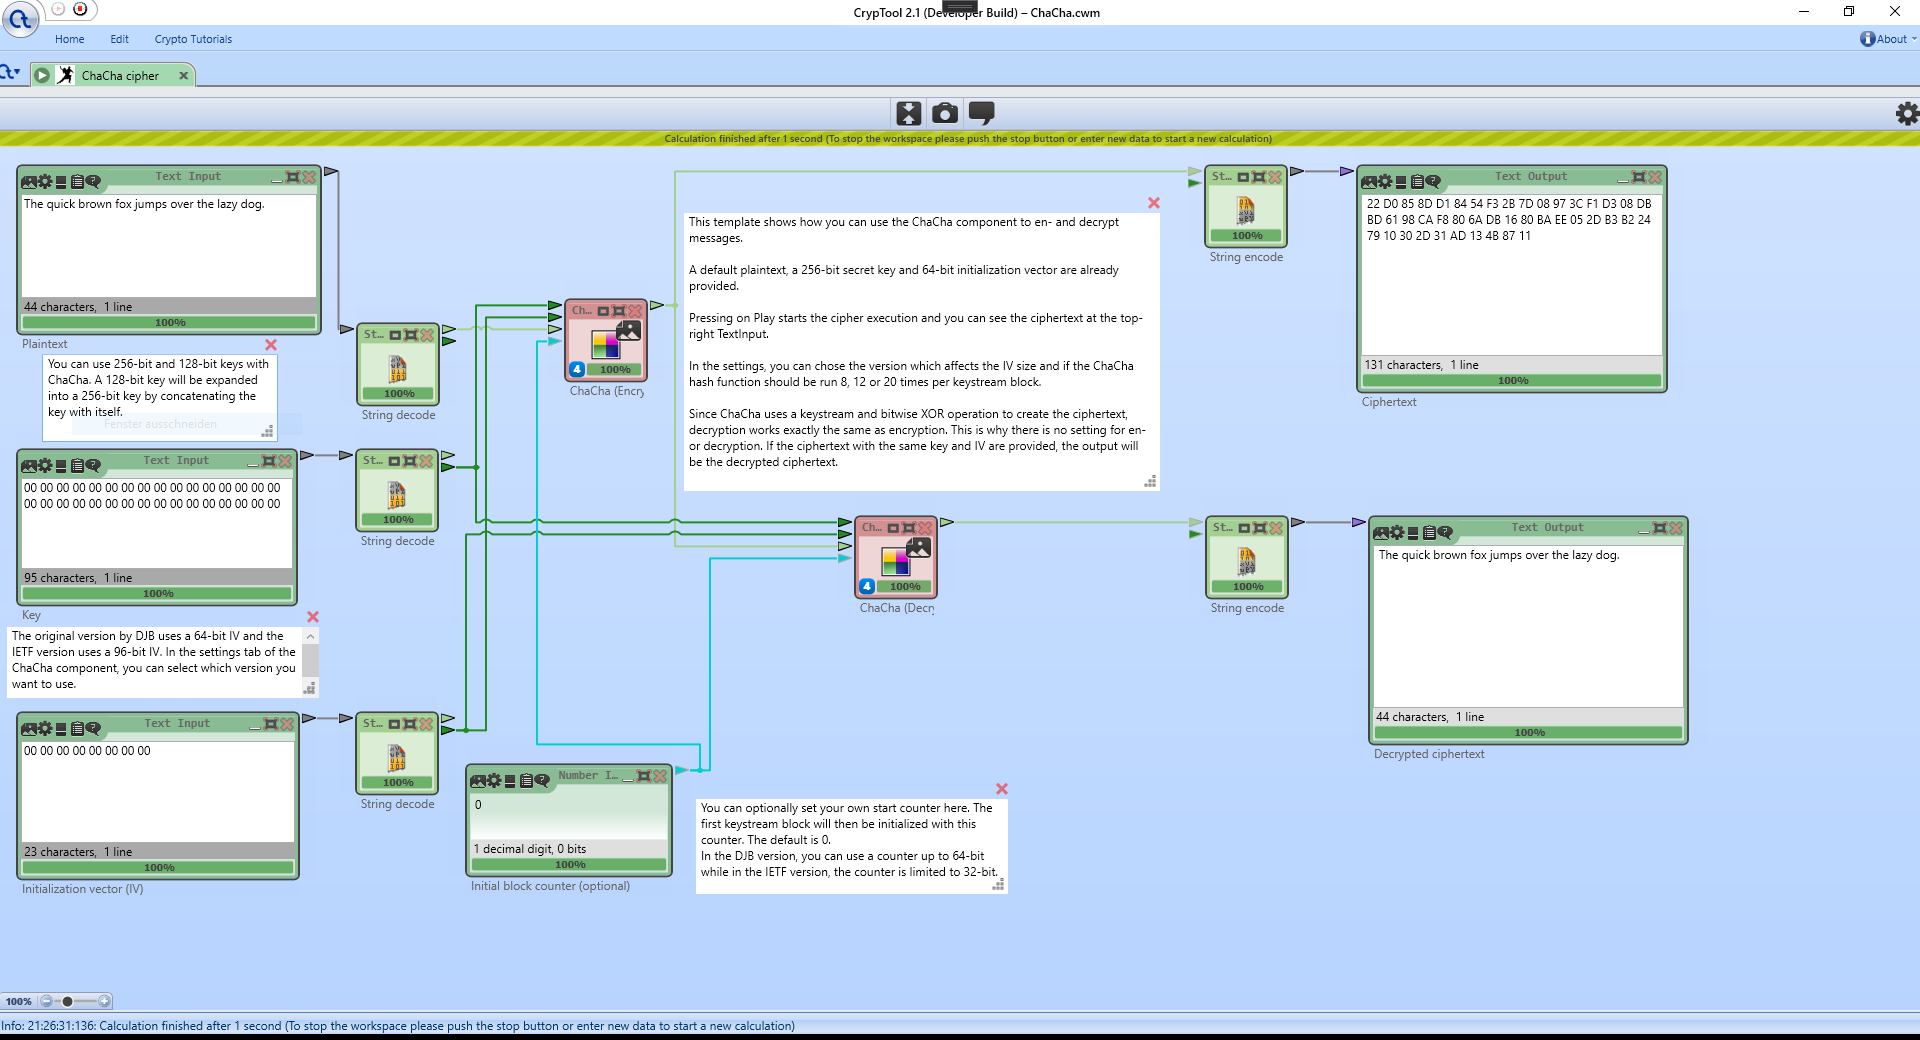
\includegraphics[width=\textwidth]{figures/ct2/plugin-template.png}
\end{figure}

The plugin offers the user the ability to input his own plaintext, key, initialization vector and initial counter using the concept of visual programming (around which CT2 is built) as one can see in Figure \ref{fig:plugin.template}. The counter is optional and defaults to $0$. These values are then used to visualize the cipher execution comprehensively. Descriptions complement the visualization by providing information about what is happening. \\
As mentioned in Section \ref{sec:goals}, if the user wants to see the diffusion property of the cipher, he can enter secondary values on a dedicated page inside the plugin. This is shown in Figure \ref{fig:diffusion}. \\
The version (original DJB version or IETF version) and how often the ChaCha hash function should be run per keystream block can be chosen in the plugin settings.

\subsection{User Interface}
\label{sec:userInterface}

\subsubsection{General interface structure}

\begin{figure}
\caption{All pages of the ChaCha visualization plugin in their initial state}
\label{fig:allpages}
\centering
\begin{subfigure}{.5\textwidth}
  \centering
  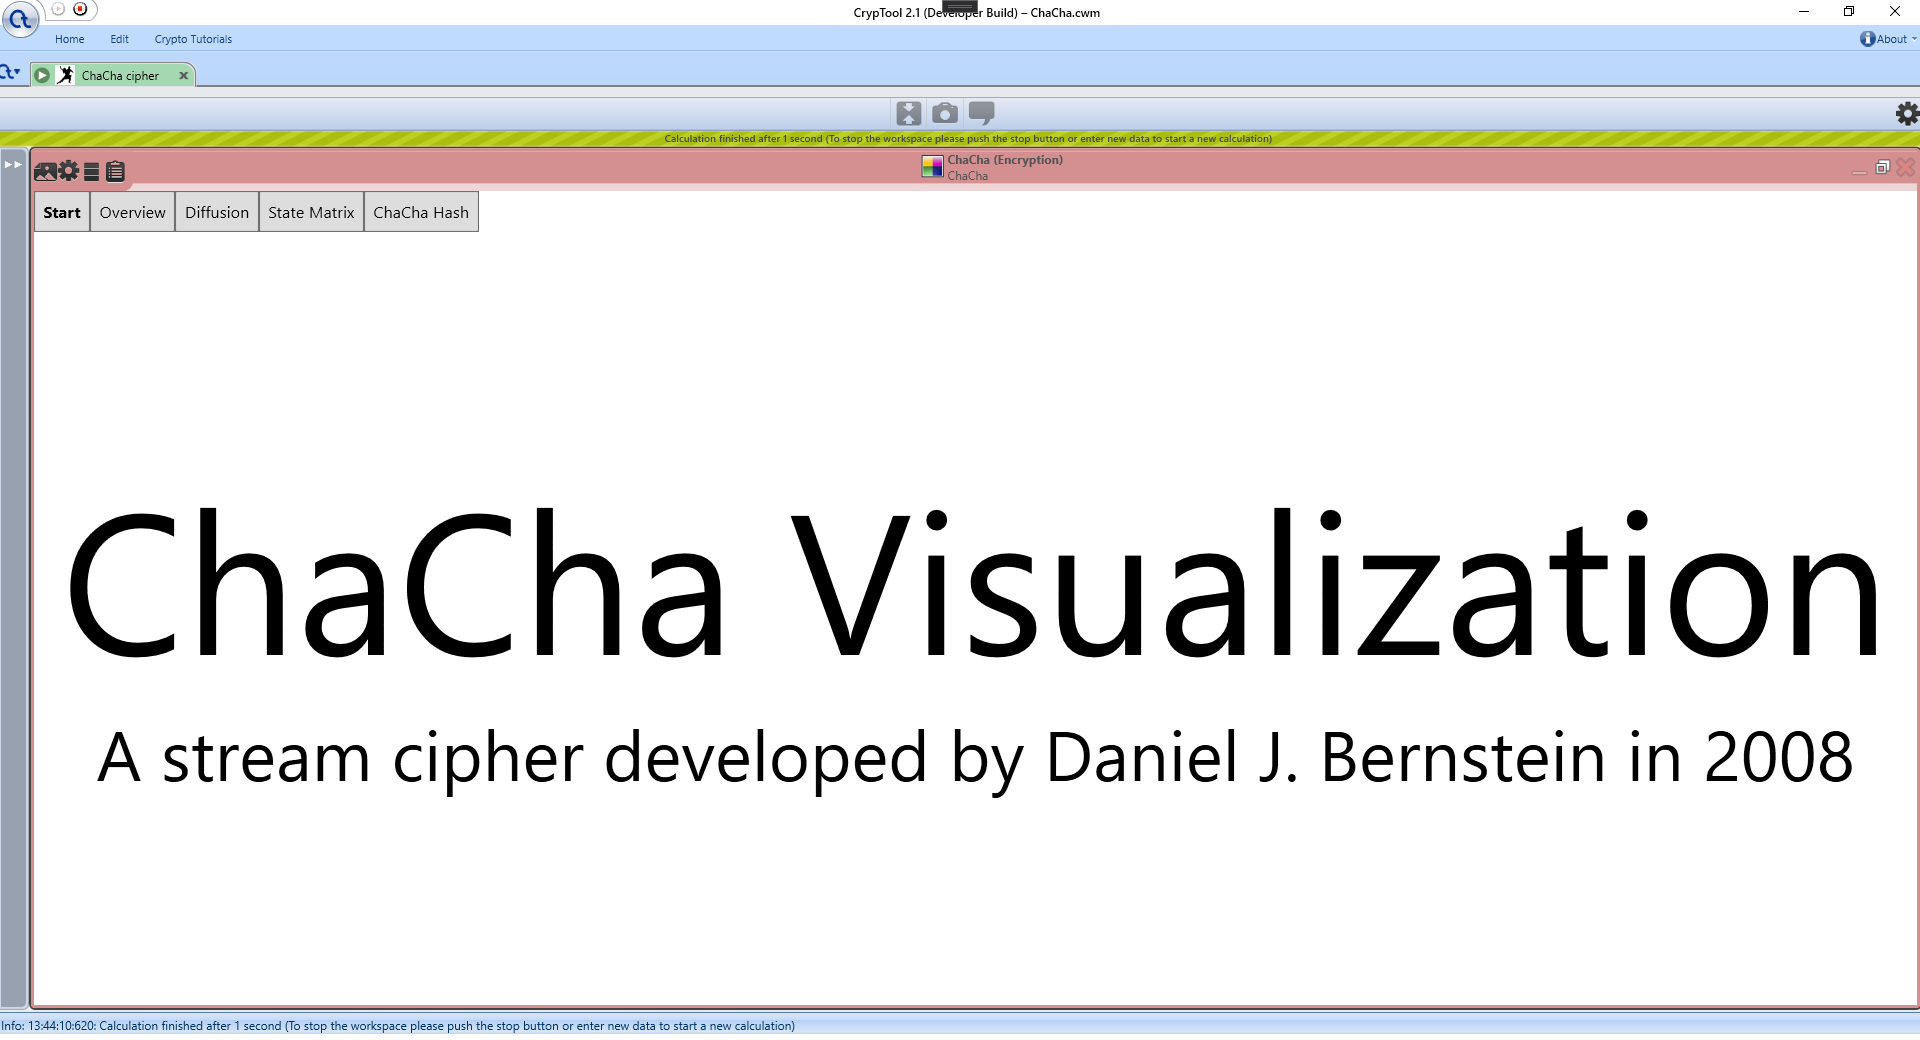
\includegraphics[width=0.99\textwidth]{figures/ct2/all-pages/1-start.png}
  \caption{Start page}
\end{subfigure}%
\begin{subfigure}{.5\textwidth}
  \centering
  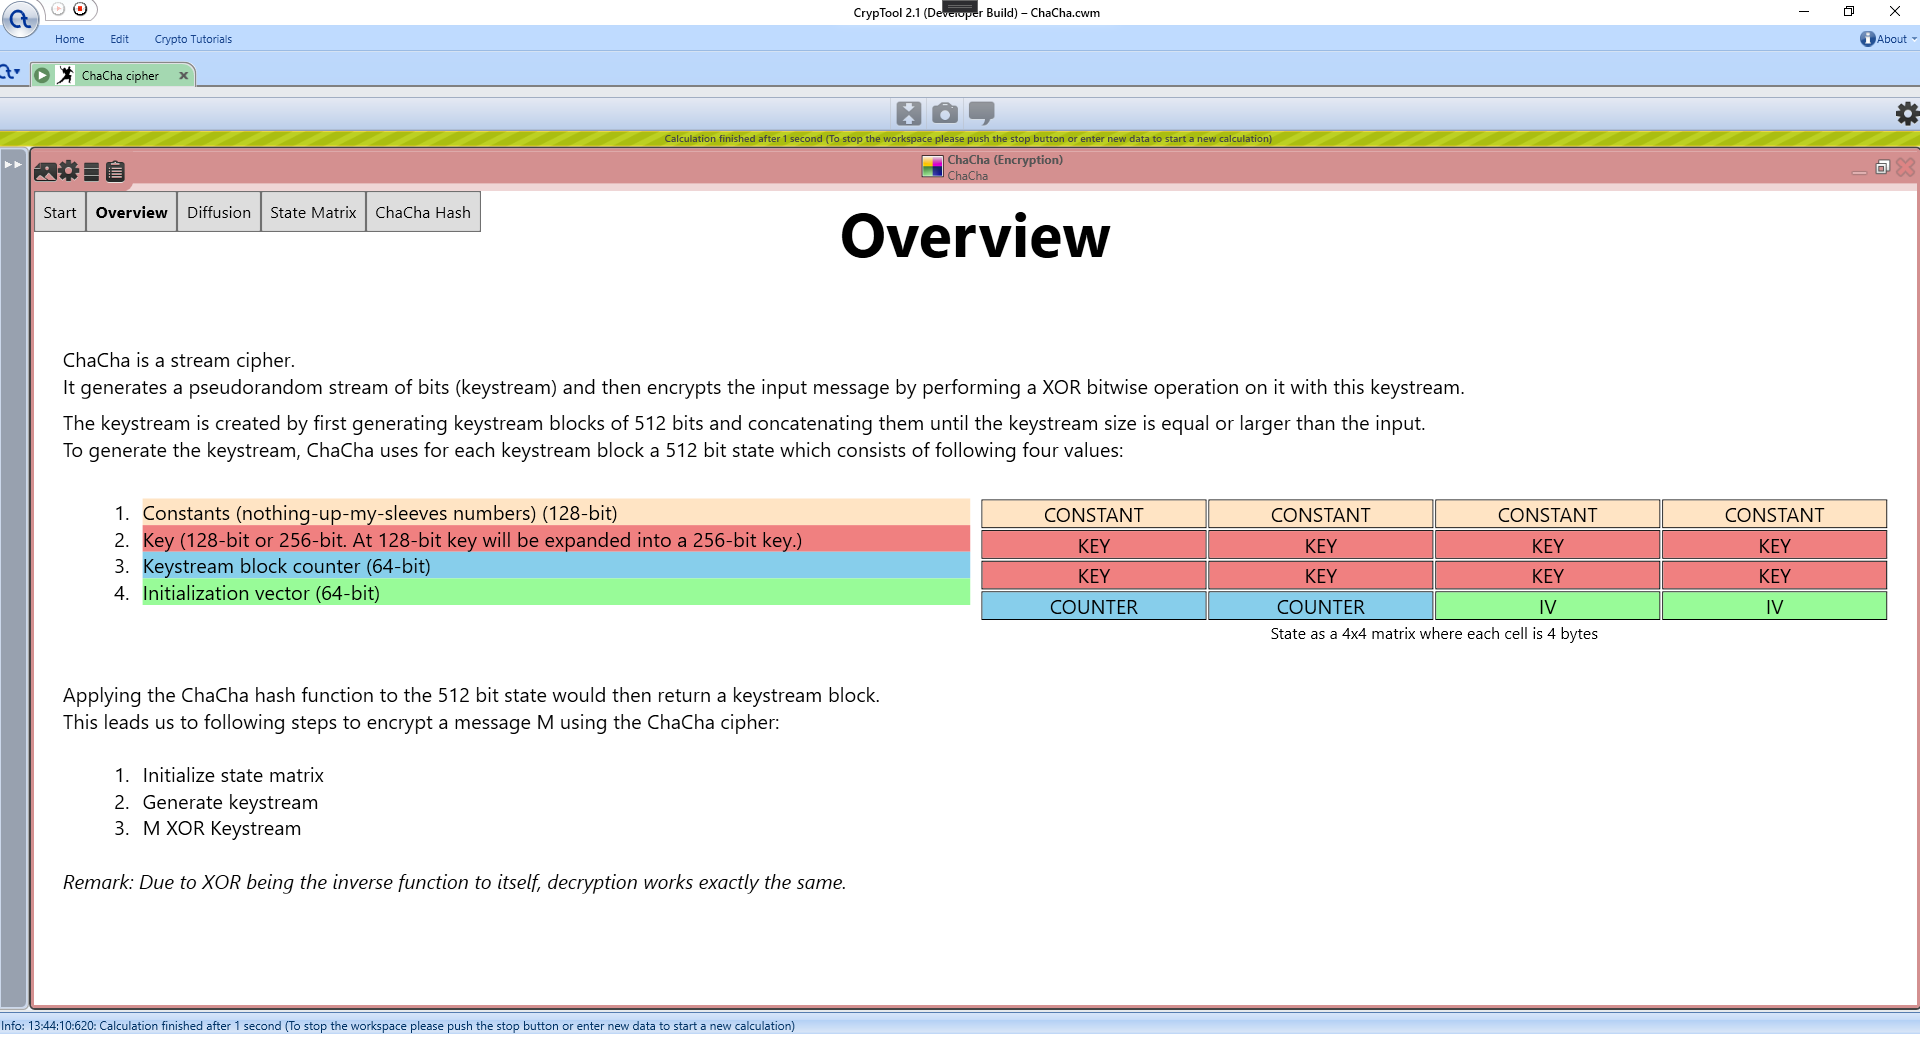
\includegraphics[width=0.99\textwidth]{figures/ct2/all-pages/2-overview.png}
  \caption{Overview page}
\end{subfigure}
\begin{subfigure}{.5\textwidth}
  \centering
  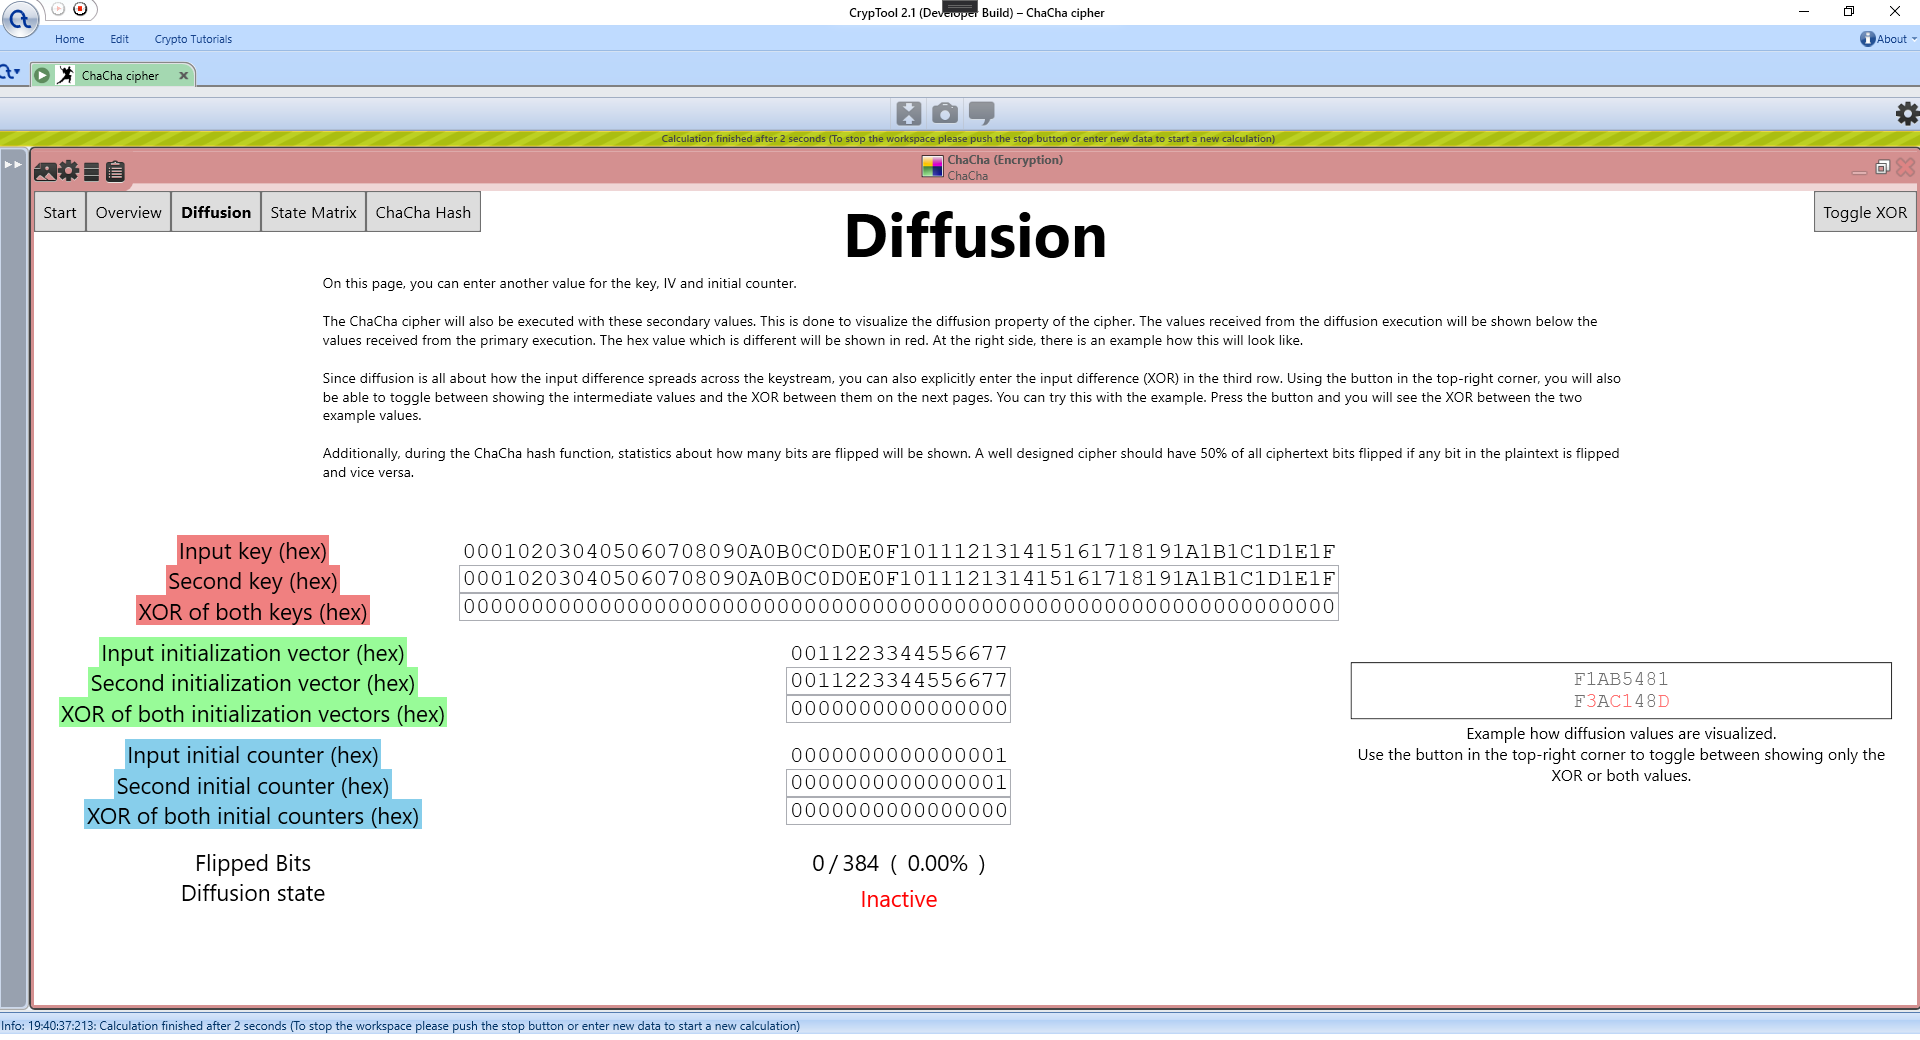
\includegraphics[width=0.99\textwidth]{figures/ct2/all-pages/3-diffusion.png}
  \caption{Diffusion page}
\end{subfigure}%
\begin{subfigure}{.5\textwidth}
  \centering
  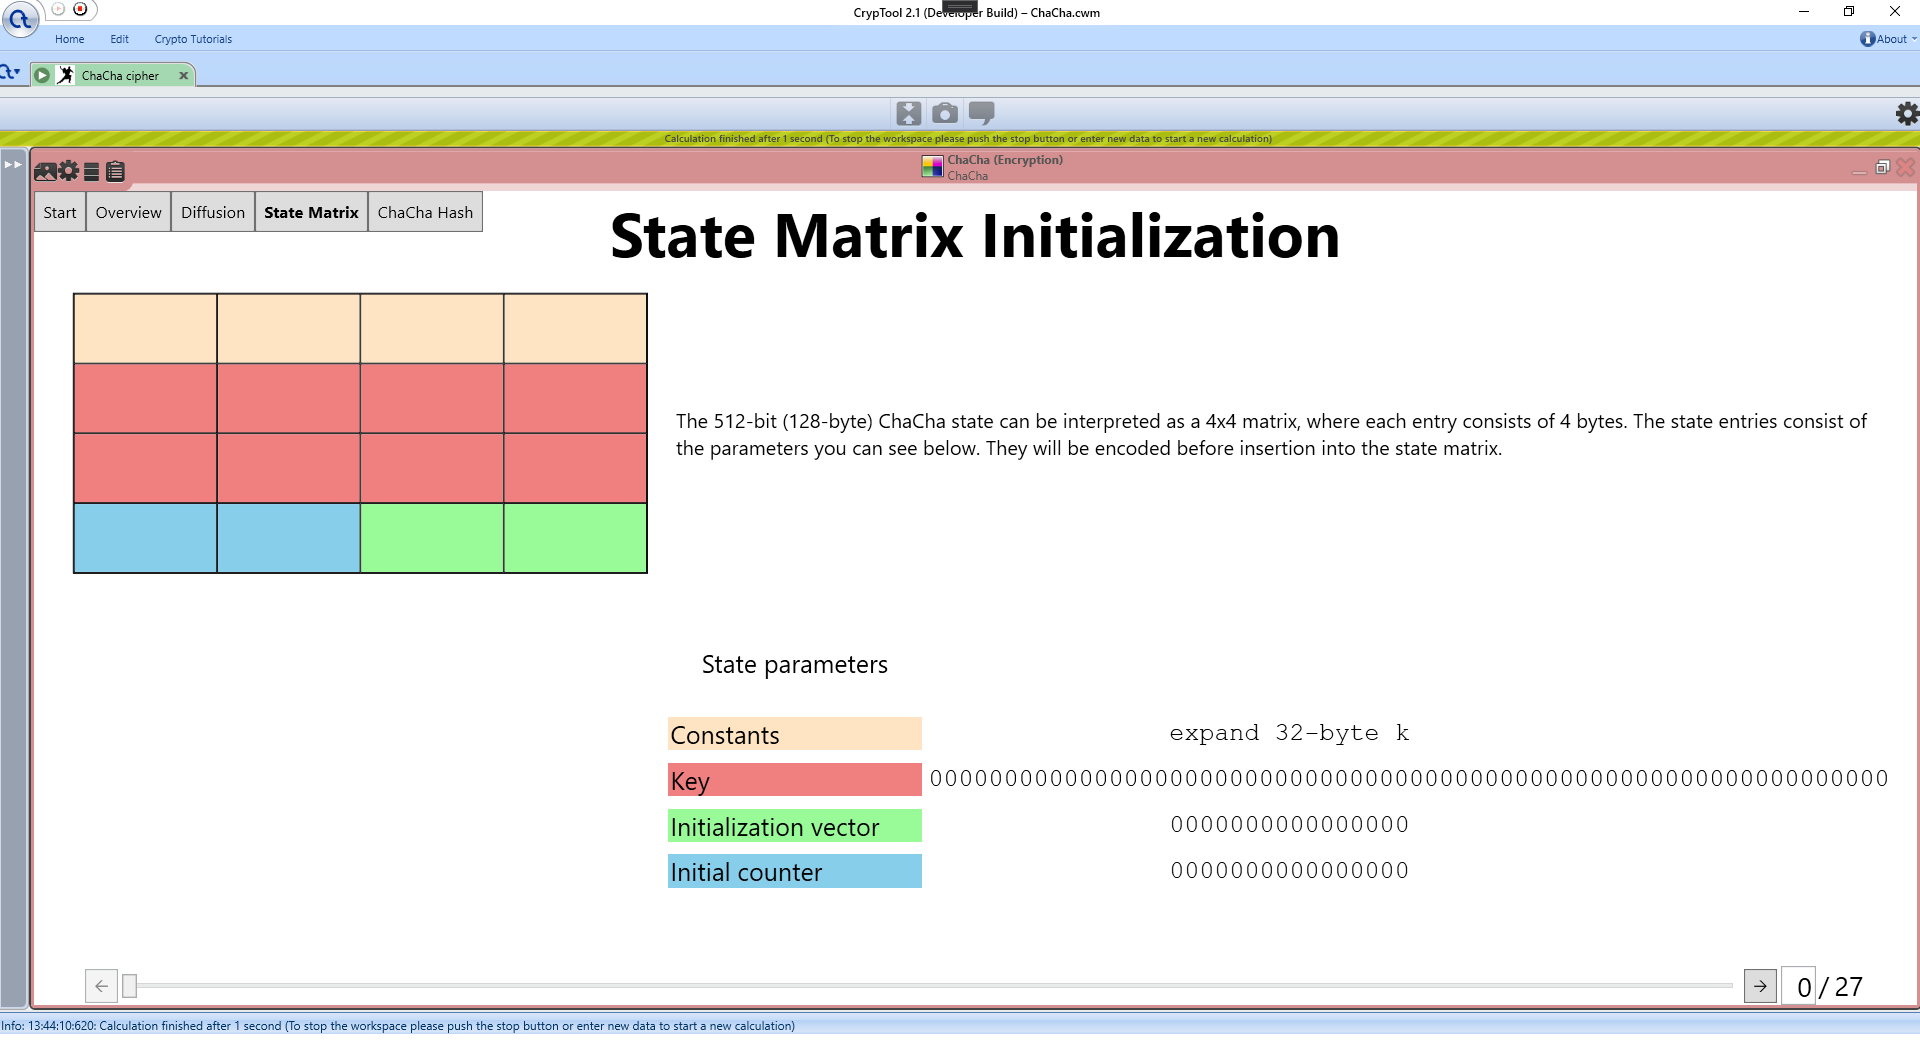
\includegraphics[width=0.99\textwidth]{figures/ct2/all-pages/4-statematrix.png}
  \caption{State Matrix Initialization page}
\end{subfigure}
\begin{subfigure}{.5\textwidth}
  \centering
  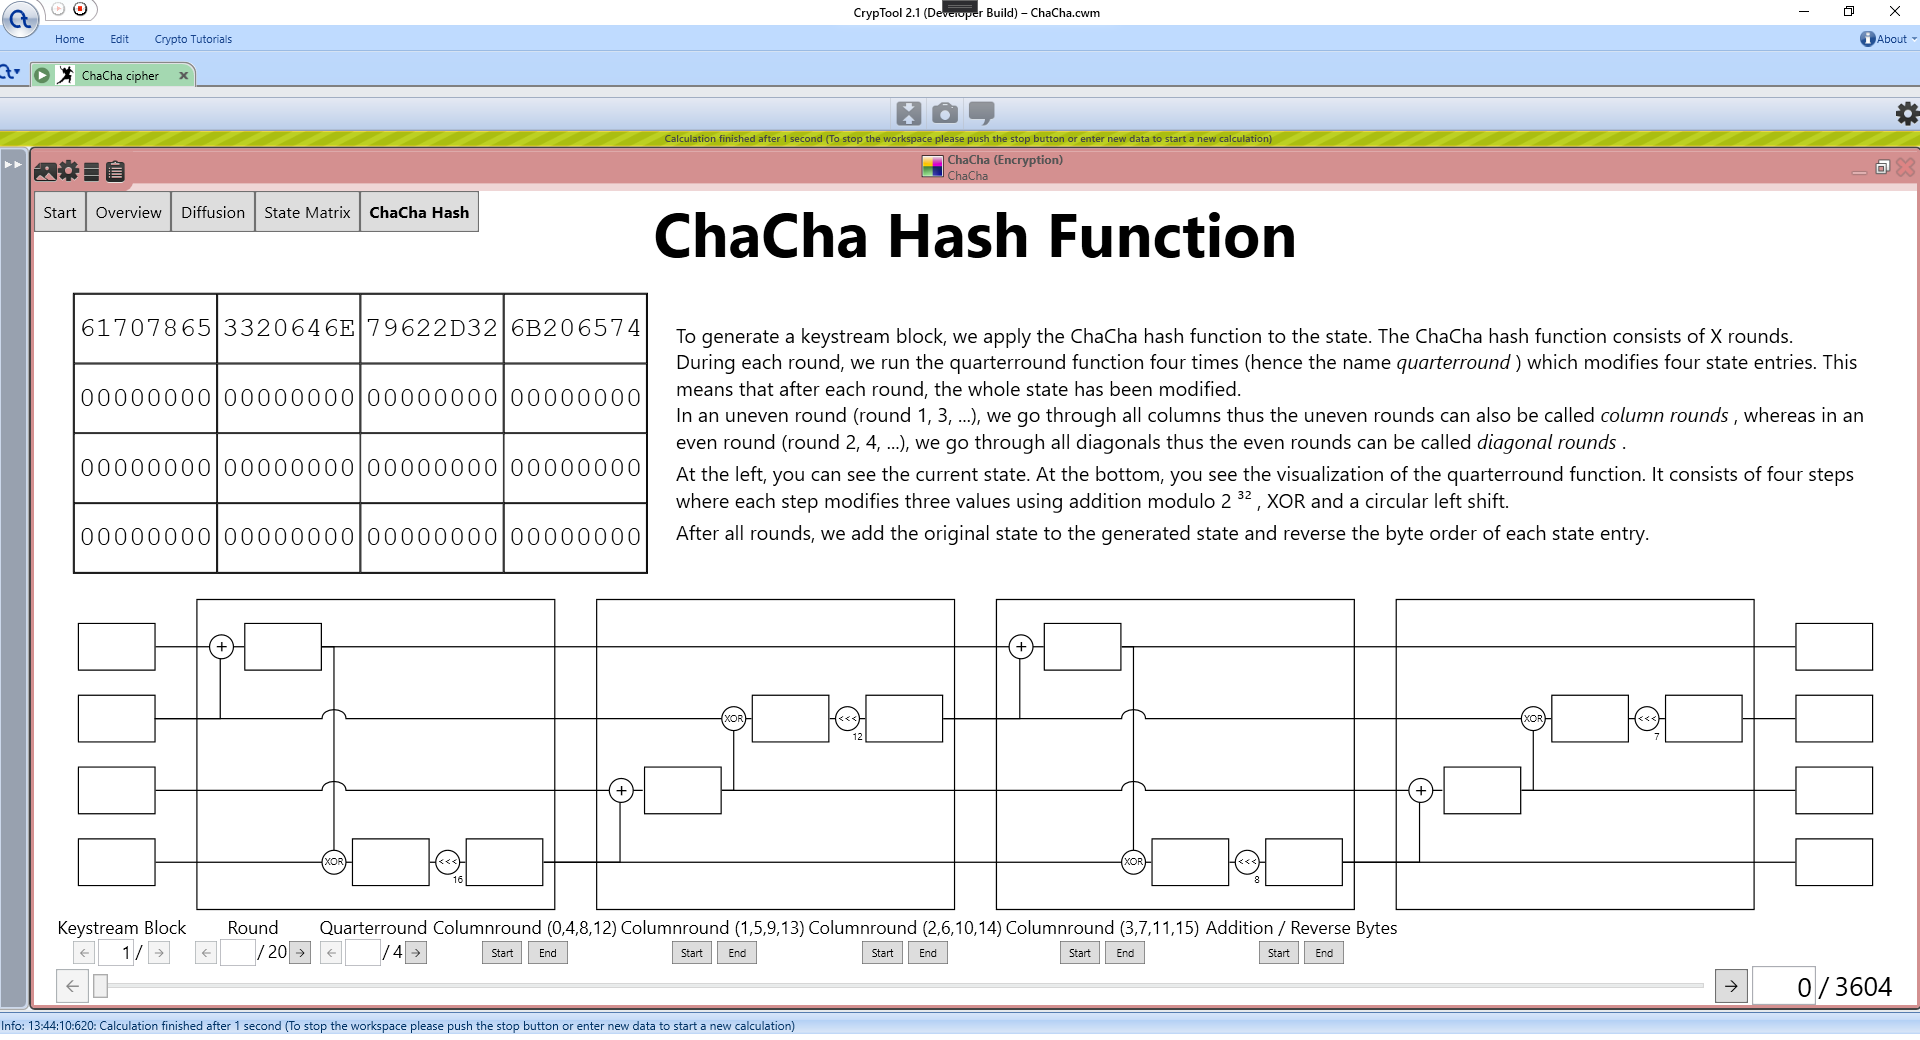
\includegraphics[width=0.99\textwidth]{figures/ct2/all-pages/5-chachahash.png}
  \caption{ChaCha Hash Function page}
\end{subfigure}
\end{figure}

All pages have a common interface layout which consists of three sections. Each section is inside a own dedicated row. \\
The first section implements the navigation to move between pages. It also shows the title of the current page. \\
The second section shows the content of the current page. The content is not always static since it can change by using the action navigation bar in the bottom section.  \\
It includes buttons to go to the previous or next action, a slider for quicker action navigation, a text input to go to a given action and a indicator on which action the user currently is and how many actions there are in total on the current page. \\
I have chosen a slider over alternative solutions like individual buttons because I wanted to enable the user to quickly navigate through a page. The slider came in handy especially for the page about the ChaCha hash function where there are more than 3000 actions per keystream block. Fitting more than 3000 buttons on a single page was not feasible but would need pagination features such as showing the next set amount of buttons which would make quick navigation impossible. \\
The user can also enter a  number into the text input to the right of the slider to go to an action. But this text input is only more helpful than the slider if the user already knows the number of the action he wants to go to. If he does not, the slider creates a much better user experience. \\
If a page does not have actions, the action navigation is hidden but the space is still reserved for it to have a consistent canvas size for all pages.

I will now go into greater detail about the pages which do not have fully static content. These pages are the Diffusion page, the State Matrix Initialization page and the ChaCha Hash Function page.

\subsubsection{Diffusion page}

As already mentioned in Section \ref{sec:keyFeatures}, on the Diffusion page, the user can enter secondary values for the key, IV and initial counter in hexadecimal. They will be used to visualize the diffusion property. This means that during cipher execution, hexadecimal letters which are different are marked red. An example of this is shown on the Diffusion page at the right side (see Figure \ref{fig:diffusion}).\\
I have used hexadecimal text inputs because the alternative, individual buttons for each bit, would have resulted in a lot of buttons because the key can be 256-bit. Together with the 128-bit from the counter and IV, this would have resulted in 384 individual buttons. Furthermore, clicking on individual buttons instead of entering text was more cumbersome. {\color{red} \\
Since when studying the diffusion property of a cipher, we are more interested in the difference of values during two cipher runs instead of the actual values, the user can also explicitly input the XOR between the primary and secondary value.} \\
To help with the input, the input fields show an error message if the user entered invalid characters or a too large string since the secondary hexstring must be of equal size as the primary value. If the hex string is too short, it gets left-padded with zeroes to align it with the primary value. \\
Last but not least, the amount of flipped bits is shown in the second to last row together with a state indication in the last row if the diffusion is active or not. The diffusion is active if at least one bit was flipped.

\subsubsection{State matrix initialization page}

\begin{figure}
\caption{Diffusion page}
\label{fig:diffusion}
\centering
\begin{subfigure}{0.5\textwidth}
  \centering
  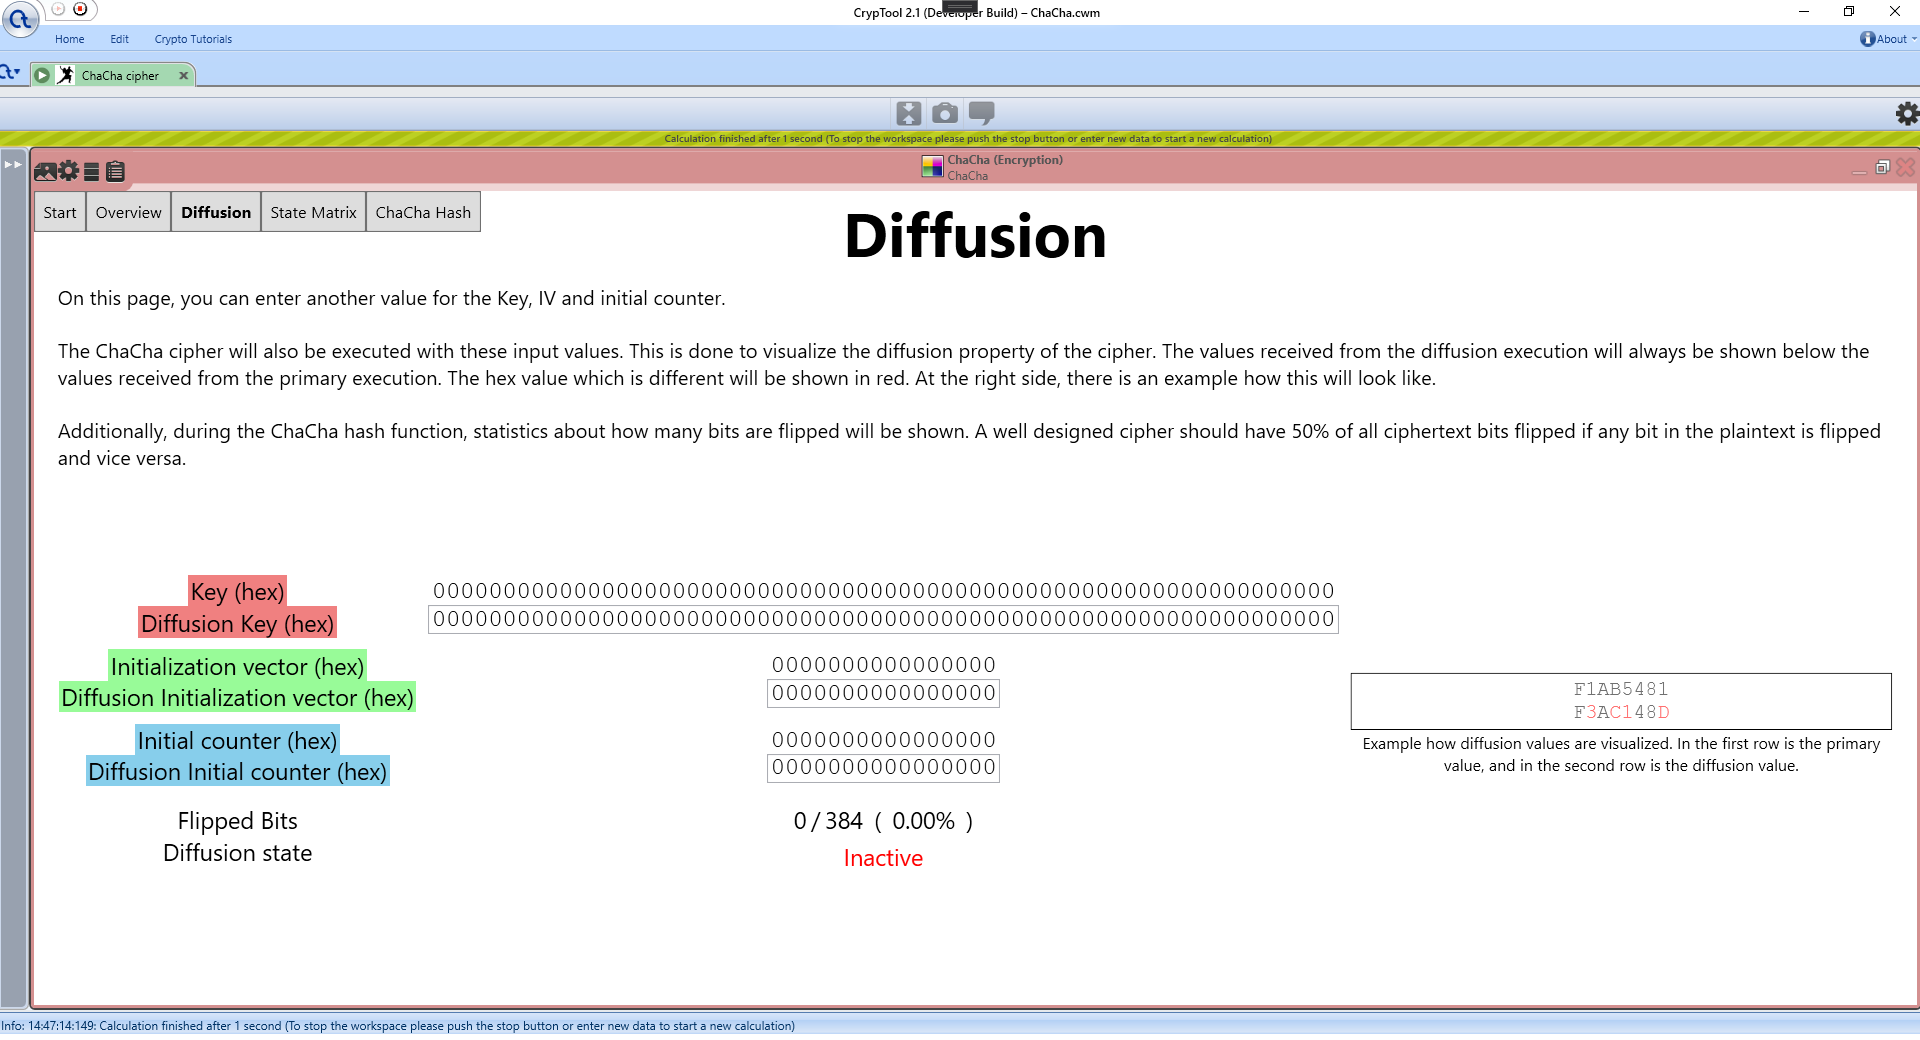
\includegraphics[width=0.99\textwidth]{figures/ct2/diffusion/diffusion-inactive.png}
  \caption{Diffusion inactive (no user input)}
  \label{fig:diffusion.inactive}
\end{subfigure}%
\begin{subfigure}{0.5\textwidth}
  \centering
  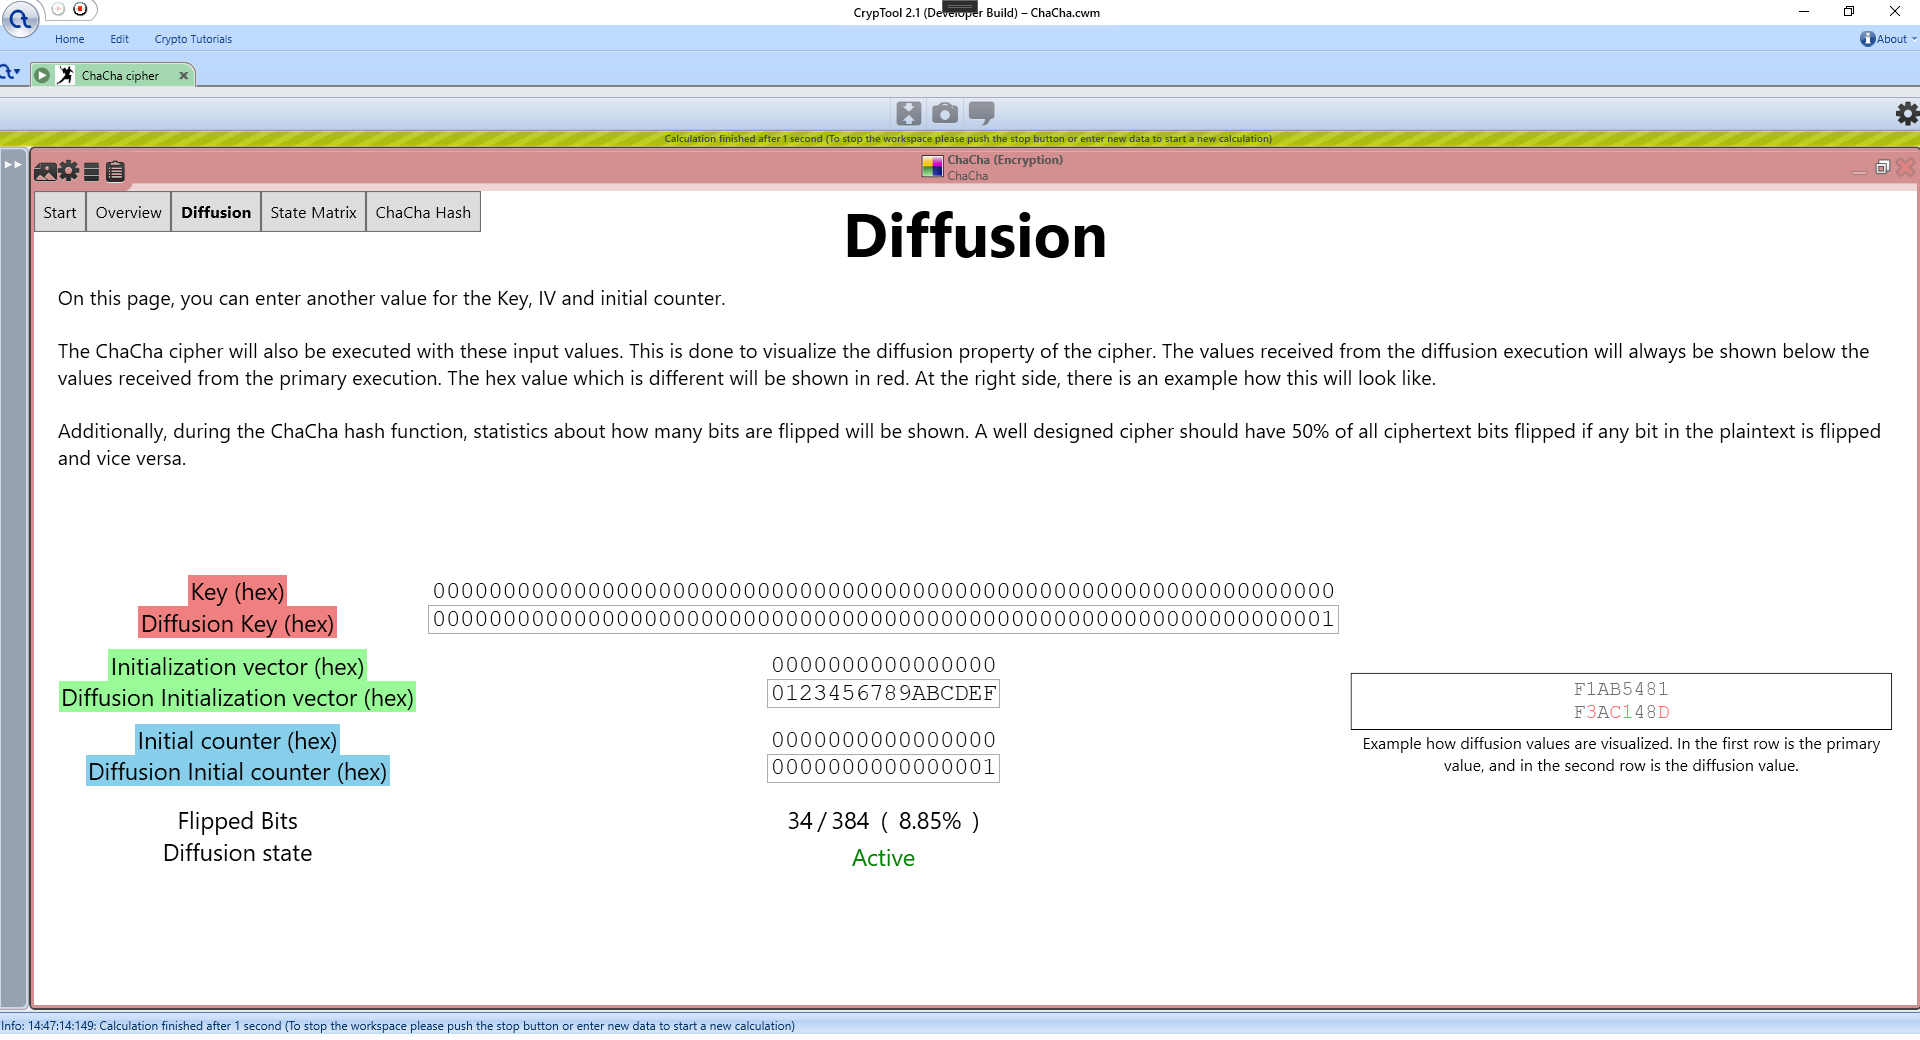
\includegraphics[width=0.99\textwidth]{figures/ct2/diffusion/diffusion-active.png}
  \caption{Diffusion active}
  \label{fig:diffusion.active}
\end{subfigure}

\caption{Encoding of the state parameters on the State Matrix Initialization page}
\label{fig:statematrix.encoding}
\begin{subfigure}{0.5\textwidth}
  \centering
  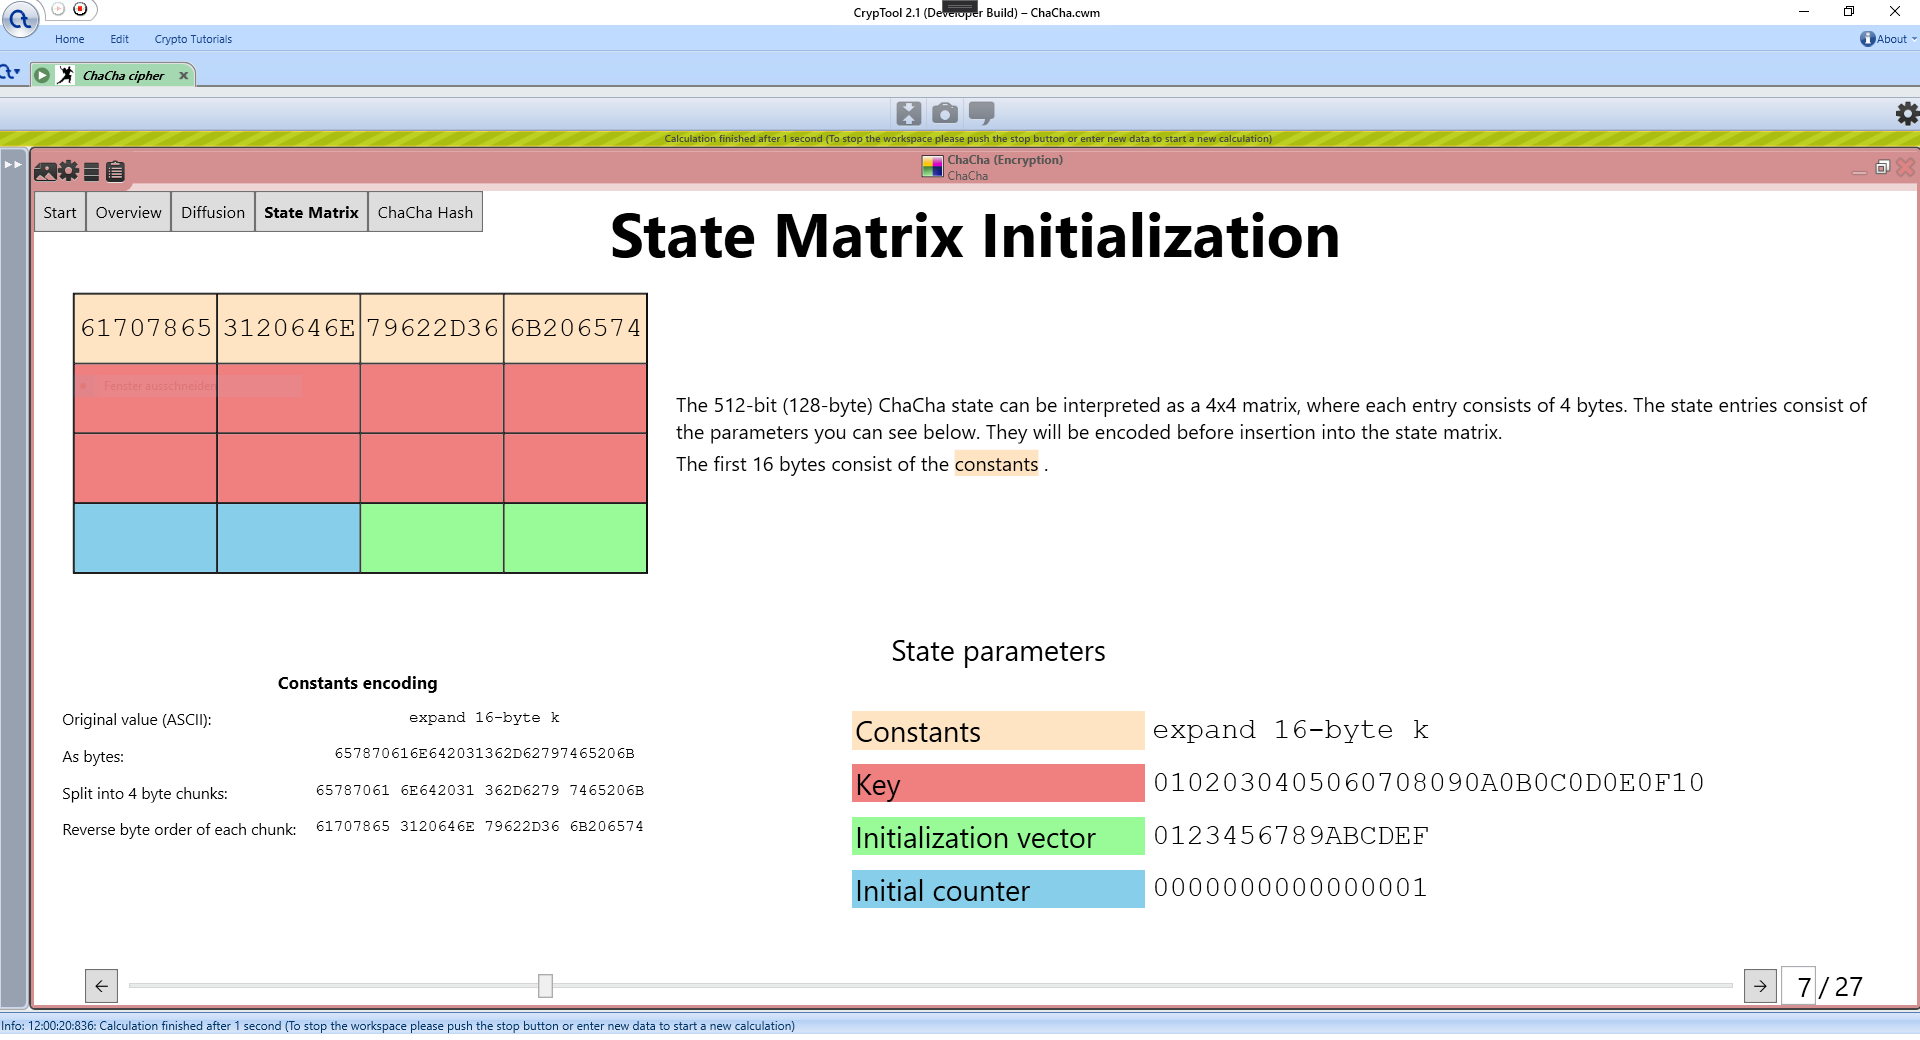
\includegraphics[width=0.99\textwidth]{figures/ct2/state-matrix/1-state-matrix-constants.png}
  \caption{Constants encoding}
  \label{fig:statematrix.encoding.constants}
\end{subfigure}%
\begin{subfigure}{0.5\textwidth}
  \centering
  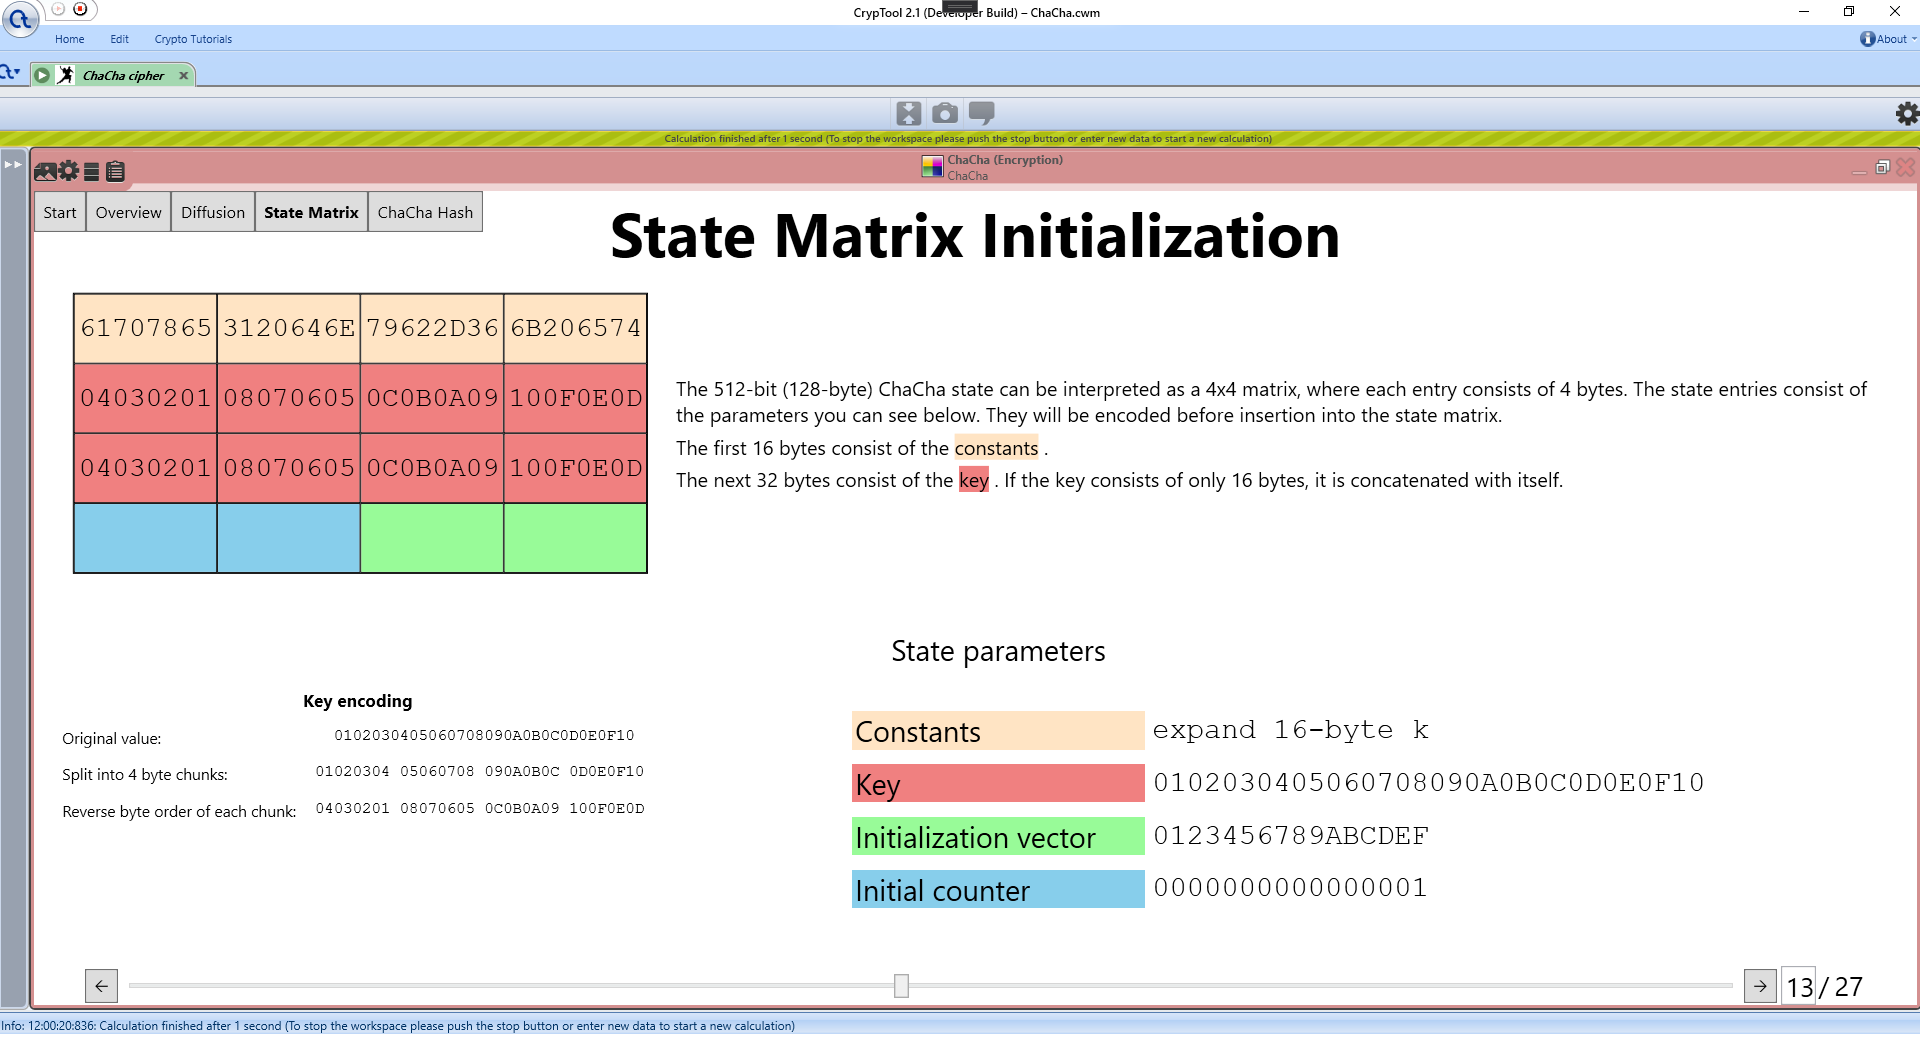
\includegraphics[width=0.99\textwidth]{figures/ct2/state-matrix/2-state-matrix-key.png}
  \caption{Key encoding}
  \label{fig:statematrix.encoding.key}
\end{subfigure}
\begin{subfigure}{0.5\textwidth}
  \centering
  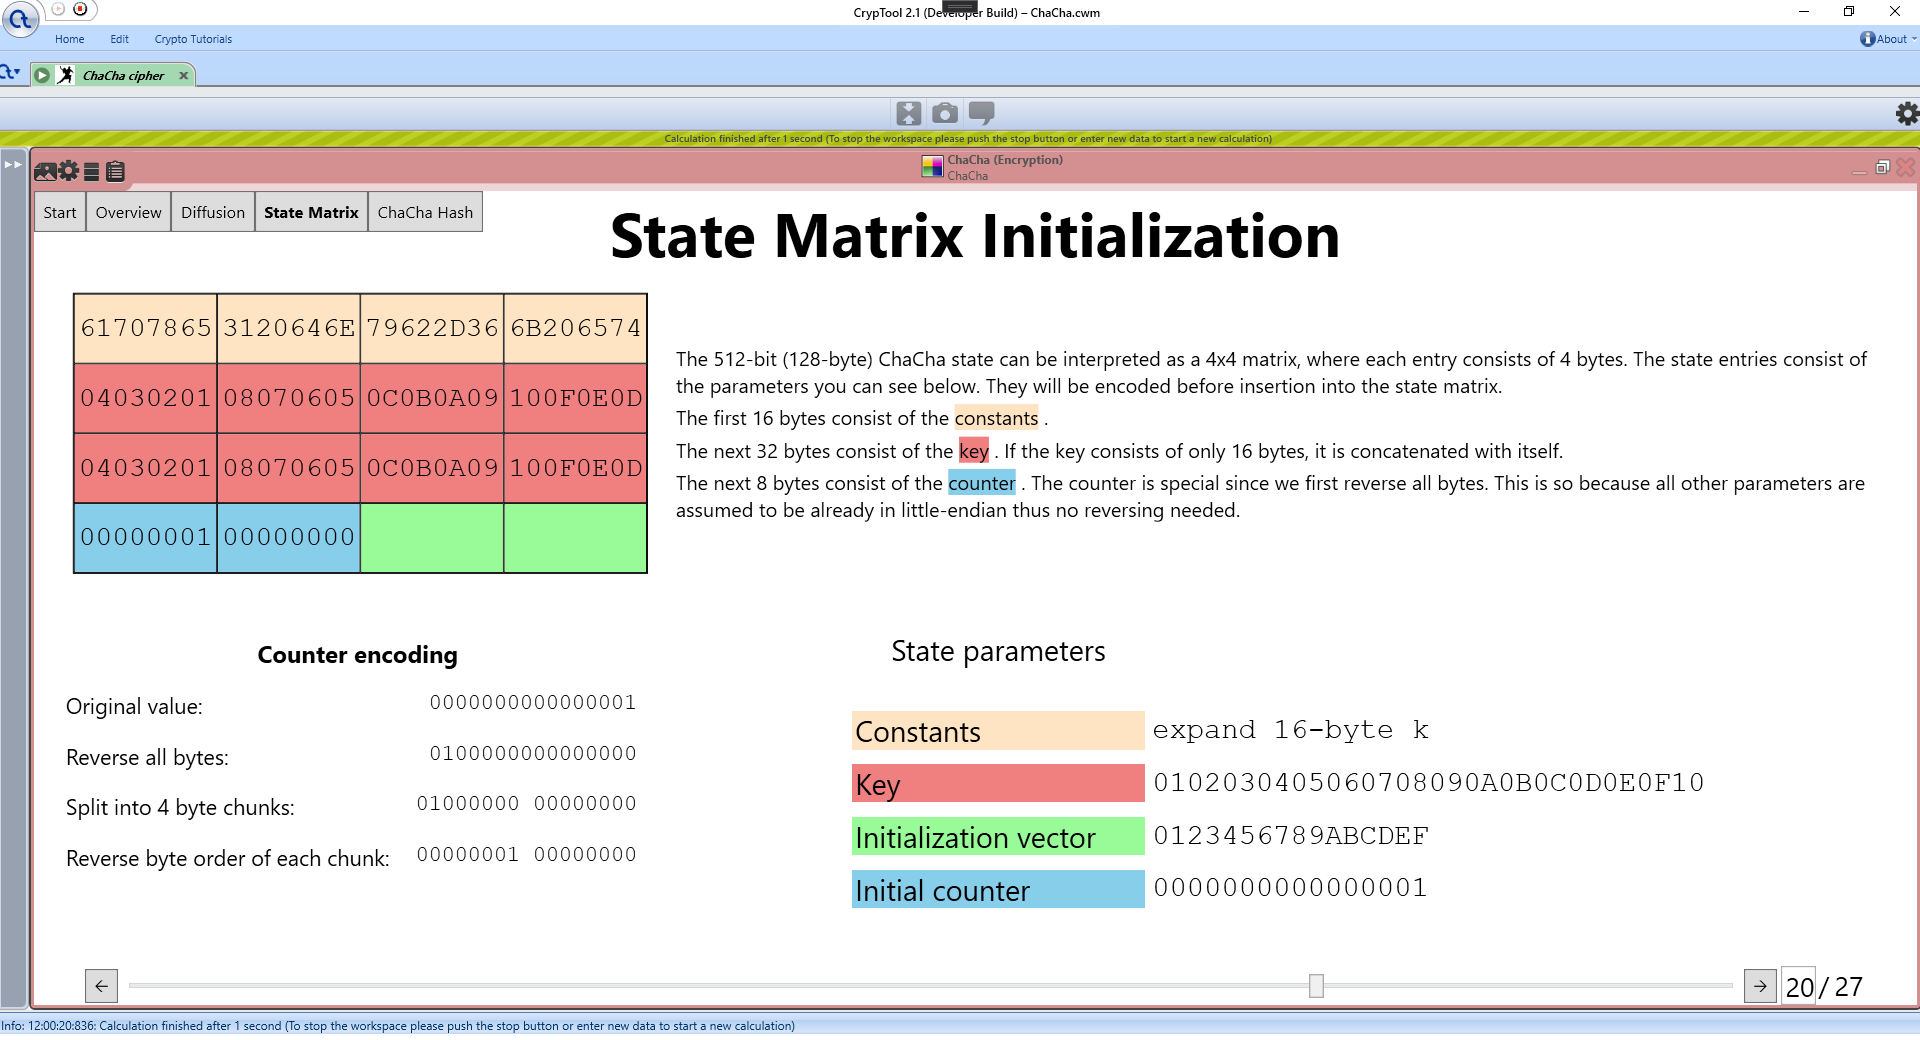
\includegraphics[width=0.99\textwidth]{figures/ct2/state-matrix/3-state-matrix-counter.png}
  \caption{Counter encoding}
  \label{fig:statematrix.encoding.counter}
\end{subfigure}%
\begin{subfigure}{0.5\textwidth}
  \centering
  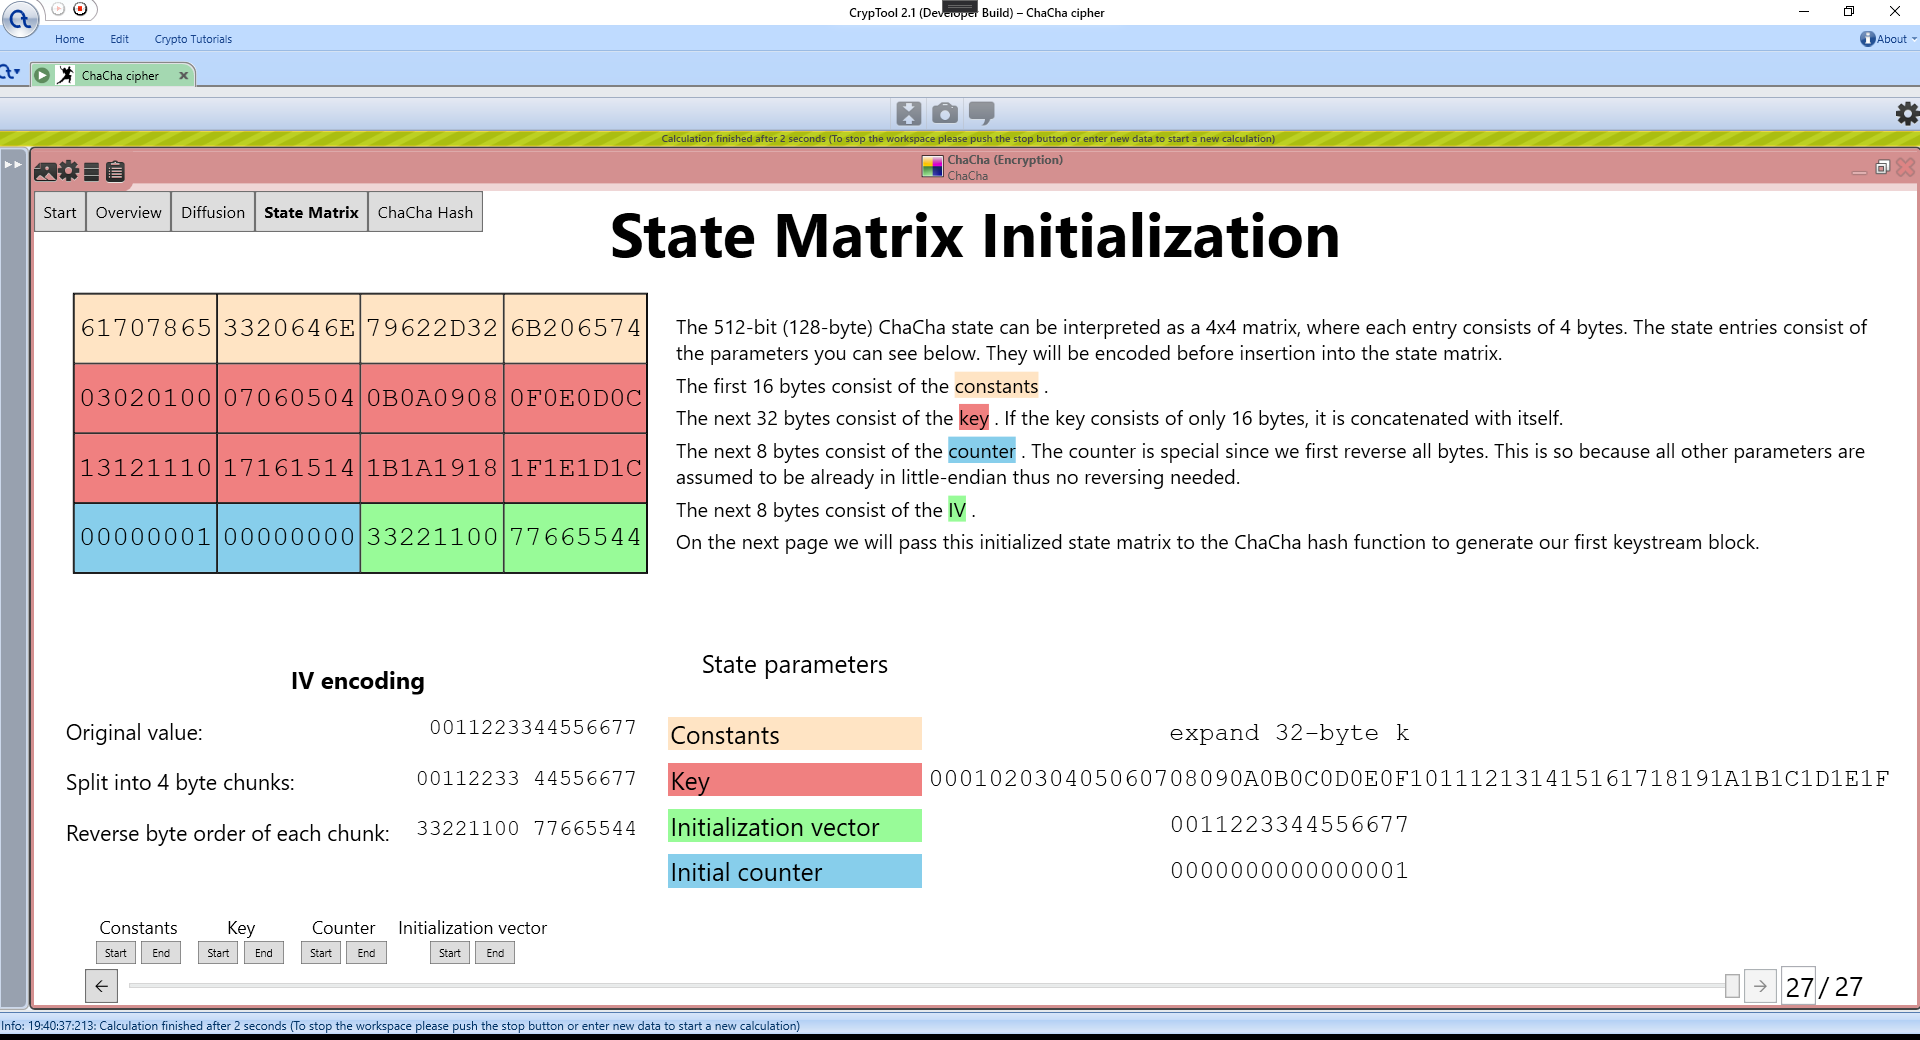
\includegraphics[width=0.99\textwidth]{figures/ct2/state-matrix/4-state-matrix-iv.png}
  \caption{IV encoding}
  \label{fig:statematrix.encoding.iv}
\end{subfigure}
\end{figure}

On the State Matrix Initialization page, it is shown how the initial 512-bit state for the first keystream block is build up. The generation of the next keystream blocks start with the same state but just with a different counter (as was described in Chapter \ref{chap:chacha}). \\
This means that only the construction of the state for the very first keystream block is shown in this page. This was done this way because I wanted to focus on one thing inside a page. I did not want to disrupt the flow of the ChaCha Hash Function page by jumping back to the visualization of the state matrix initialization just to encode a different counter. The information which is provided to the user in the first and only state matrix initialization should be enough for him to construct all following initial states without further guidance. \\
Therefore, I focused on a comprehensive visualization of the encoding for each state parameter (constants, key, IV, counter). In Figure \ref{fig:statematrix.encoding}, you can see the page state during the end of each state parameter encoding. In the top-left inside each picture, you see the state. On the top-right, you see descriptions which inform the user about what the next steps are.
At the bottom-left, the encoding is visualized. At the bottom-right, the state parameters with their original values before encoding are shown.\\
For each encoding step which corresponds to a row in the encoding section, a page action has been implemented. This means that the user can follow along each encoding step-by-step in his own speed and is not overwhelmed by a lot of information.\\
First, the constants are encoded. Since they are shown in ASCII format in the state parameters section, they are first decoded to show the actual byte values. Then the bytes are split into 4 byte chunks whose order is then reversed in the last step. \\
Afterwards, the key is encoded. It is just split into 4 byte chunks whose order is then reversed. \\
When encoding the counter, the complete byte order is first reversed, and then it is split into 4 byte chunks whose byte order is then again reversed. \\
The last parameter is the IV. It is encoded exactly the same as the key. \\

\subsubsection{ChaCha hash function page}

The ChaCha Hash Function page visualizes the generation of a keystream block by using two kind of visualizations: The quarterround visualization  and the addition / reverse bytes step at the end of the hash function. \\
At the top, you can see the current state together with a description about the ChaCha hash function.\\
At the bottom, if we are still in the ChaCha hash function loop, you can see the visualization of the quarterrounds (Figure \ref{fig:chachahash.mid.qr}). The quarterround visualization is split into four cells on either side and four boxes in the middle . The boxes on the two ends contain the four input and output values of the quarterround. The boxes in the middle visualize one quarterround step as was described in Section \ref{sec:chacha.qr}. \\
I have used a circuit diagram to visualize the quarterround similar to the one found in the ChaCha section on the Wikipedia page about Salsa20 (see Figure \ref{fig:wiki.qr.circuit}). This way, I could easily show the intermediate values by putting them on the circuit lines. Furthermore, following along the visualization was very clear because all next steps are already shown just with empty values yet. \\
If we are finished with the loop, you can see the original state at the left, the result of adding the original state with the state after all rounds in the middle, and at the right the result of reversing the byte order of each state entry of the state in the middle (Figure \ref{fig:chachahash.end}). This is the final state and thus one 512-bit block inside the keystream with which the input message is later XOR'ed . \\
Below the visualization and just above the slider for the page actions is another navigation bar. This helps the user to quickly navigate through the ChaCha hash function. He can use the arrow buttons to traverse through the keystream blocks, rounds or quarterrounds or enter a number to directly go to a specific step. \\
For example, if he wants to go to the second quarterround of the fourth round, he can enter "4" into the text input which is labeled with "Round" and press Enter or use the arrow buttons to go to the fourth round. This will take him to the start of the fourth round. He can then proceed to enter "2" into the "Quarterround" text input. \\
Since this will also take him to the start of the quarterround, he can use the buttons to the right of the quarterround input to jump to the end of specific quarterrounds of the current round. For example, if he now wants to go to the end of the second quarterround, he can click on "End" of the second button of the buttons which are labeled with "Diagonalround". \\
They also show the state indices that will get updated during their quarterround in parentheses. They also will be updated according to the round. This means on uneven rounds, the label will switch to "Columnround" and on even rounds, it will show "Diagonalround". \\
Figure \ref{fig:chachahash.cr} and Figure \ref{fig:chachahash.dr} show exemplary how the page looks like at the end of each quarterround for round 1 (column rounds) and round 2 (diagonal rounds). As you can see, the corresponding state entry is highlighted with a light blue background. This light blue background is also used throughout the visualization to catch the user's attention about which UI elements will be updated in the next step.\\

\begin{figure}
\caption{Quarterround visualization during ChaCha hash function}
\label{fig:chachahash.mid.qr}
\centering
\begin{subfigure}{\textwidth}
  \centering
  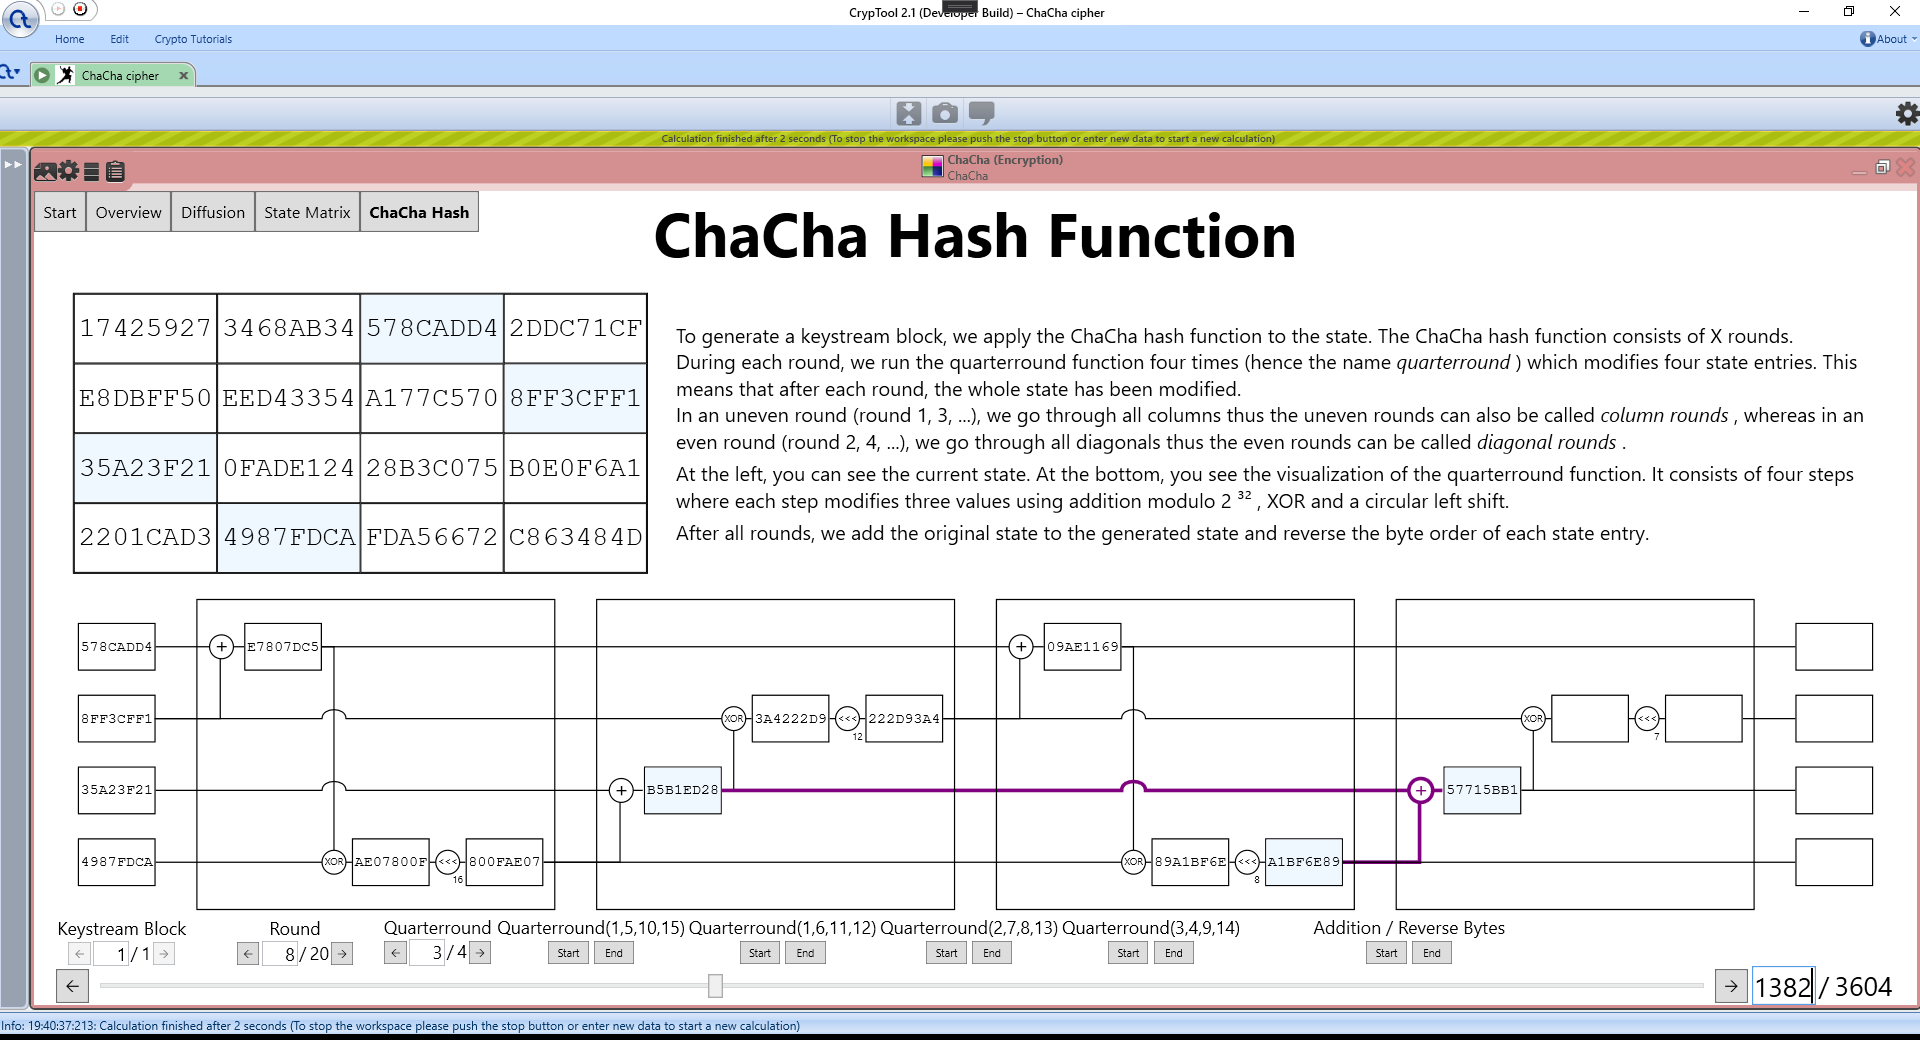
\includegraphics[width=\textwidth]{figures/ct2/chachahash/chachahash-mid-qr.png}
  \caption{Quarterround visualization (without diffusion)}
  \label{fig:chachahash.mid.qr.without.diffusion}
\end{subfigure}
\begin{subfigure}{\textwidth}
  \centering
  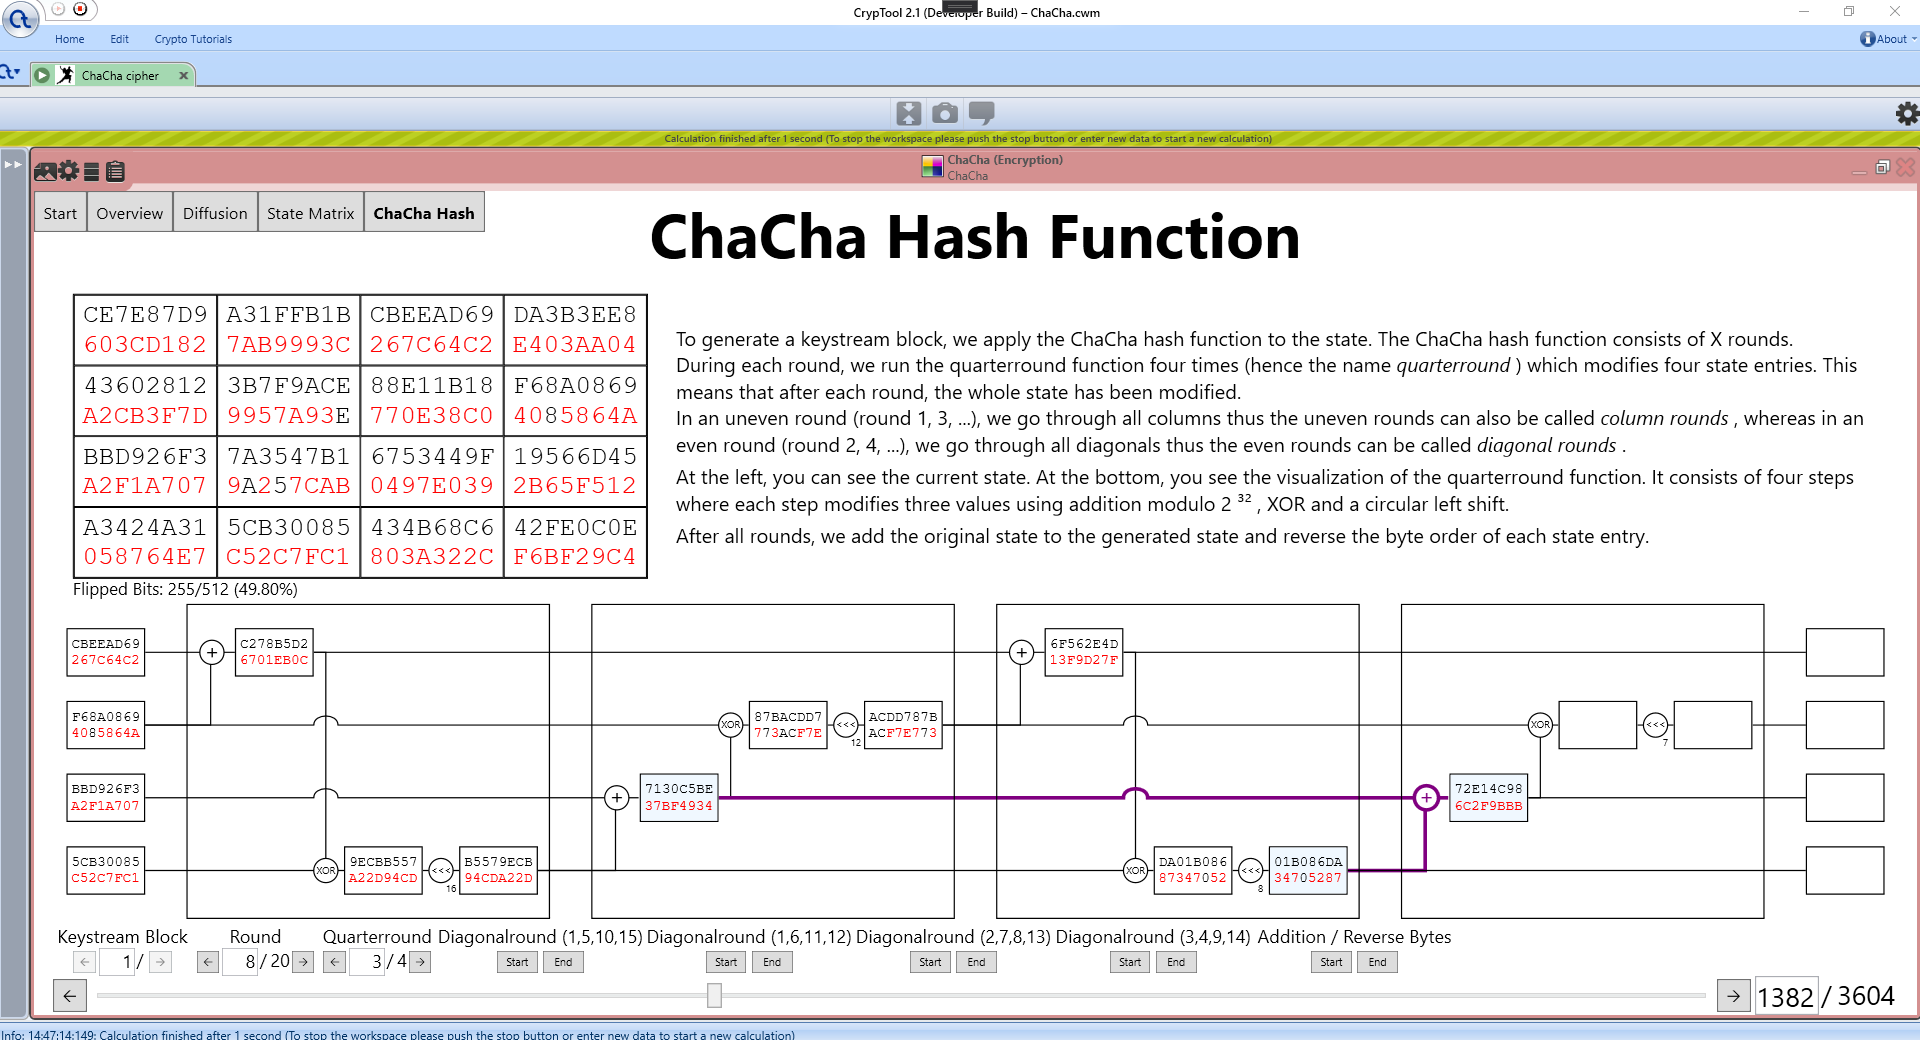
\includegraphics[width=\textwidth]{figures/ct2/chachahash/chachahash-mid-qr-diffusion.png}
  \caption{Quarterround visualization (with diffusion)}
  \label{fig:chachahash.mid.qr.with.diffusion}
\end{subfigure}
\end{figure}

\begin{figure}
\caption{Quarterround circuit diagram (Source: Wikipedia)}
\label{fig:wiki.qr.circuit}
\begin{subfigure}[t]{0.5\textwidth}
  \centering
  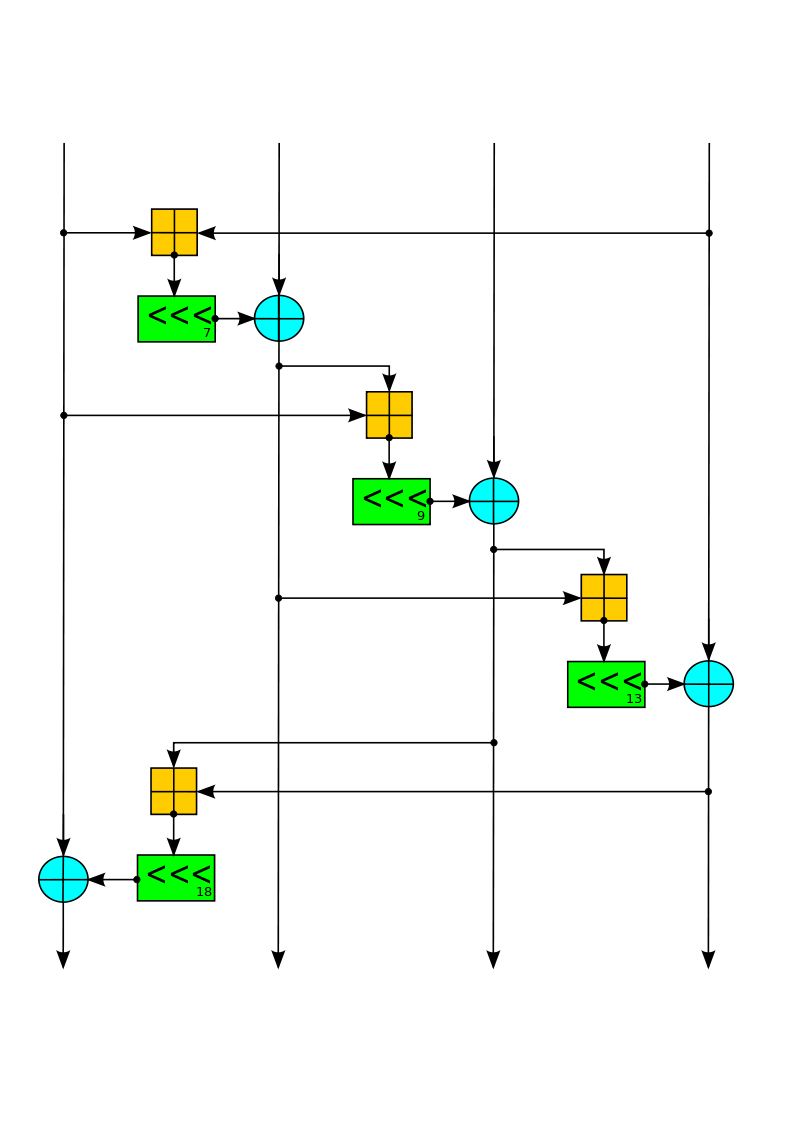
\includegraphics[width=0.99\textwidth]{figures/wiki-qr-circuit/salsa-wiki-qr-circuit.png}
  \caption{Salsa quarterround circuit diagram}
  \label{fig:wiki.qr.circuit.salsa}
\end{subfigure}%
\begin{subfigure}[t]{0.5\textwidth}
  \centering
  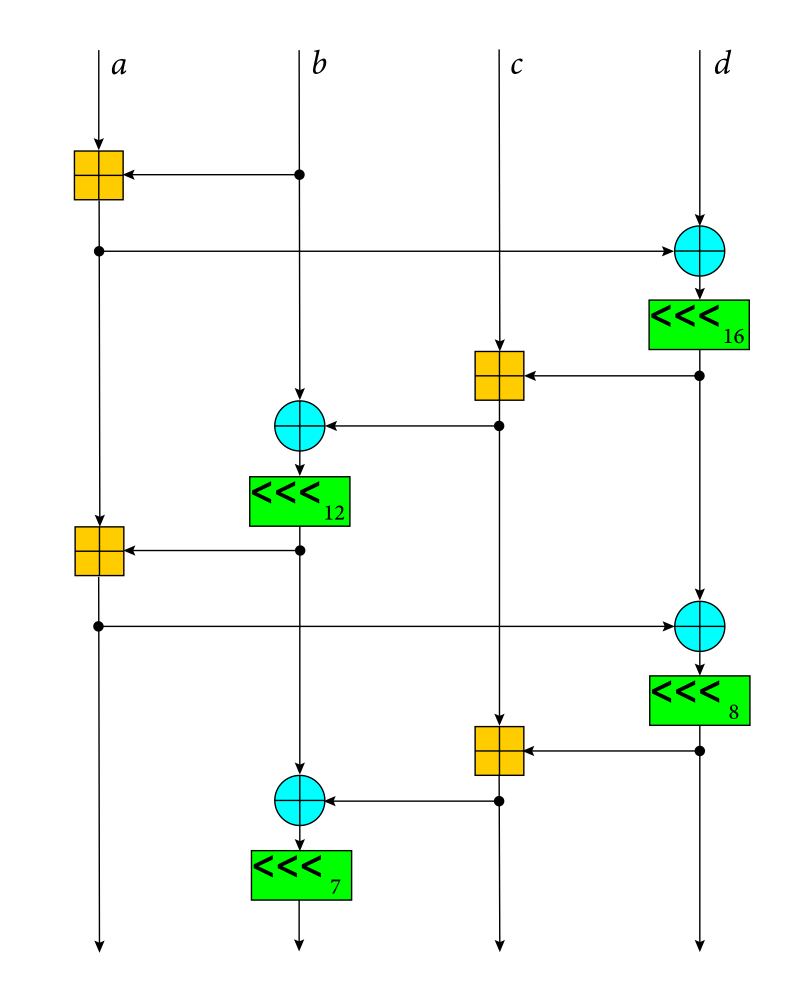
\includegraphics[width=0.99\textwidth]{figures/wiki-qr-circuit/chacha-wiki-qr-circuit.png}
  \caption{ChaCha quarterround circuit diagram}
  \label{fig:wiki.qr.circuit.chacha}
\end{subfigure}%
\end{figure}

\begin{figure}
\caption{Addition and Little-Endian step visualization at the end of the ChaCha hash function}
\label{fig:chachahash.end}
\centering
\begin{subfigure}{\textwidth}
  \centering
  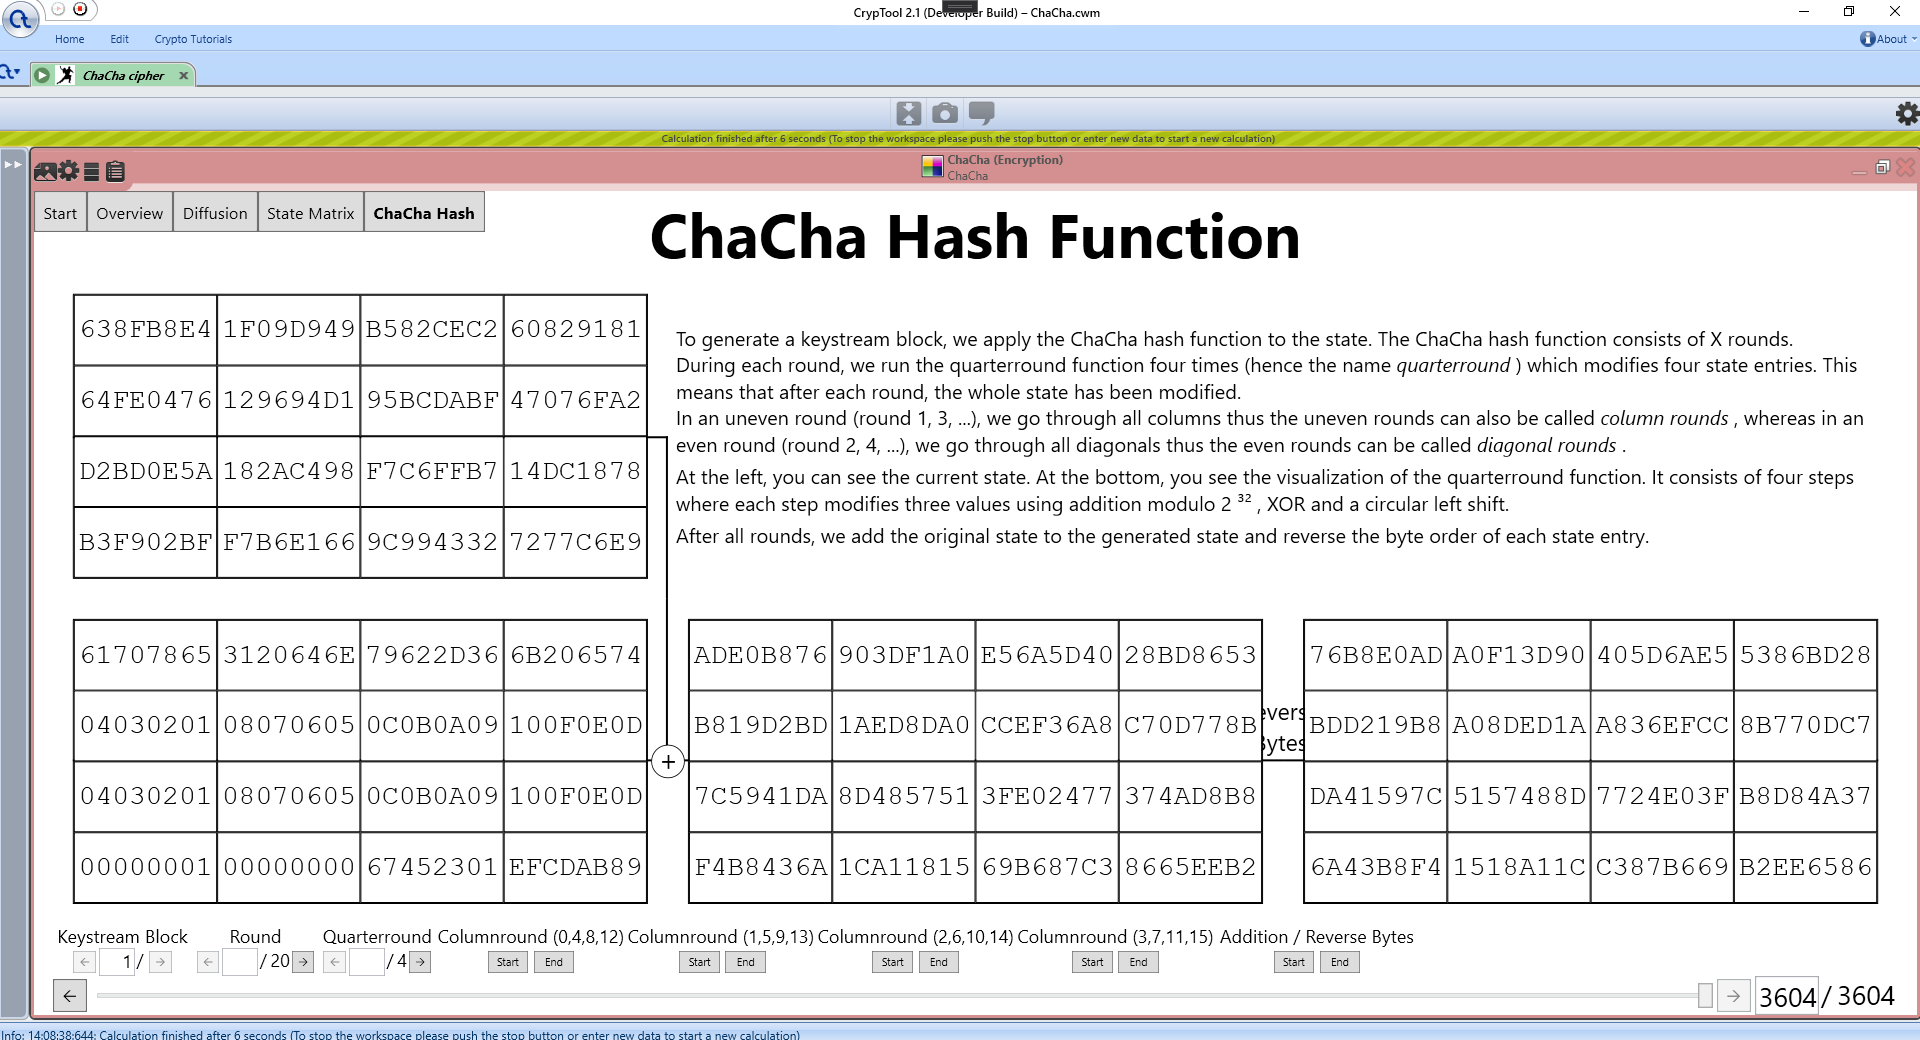
\includegraphics[width=\textwidth]{figures/ct2/chachahash/chachahash-end.png}
  \caption{Addition and Little-Endian step visualization (without diffusion)}
  \label{fig:chachahash.end.without.diffusion}
\end{subfigure}
\begin{subfigure}{\textwidth}
  \centering
  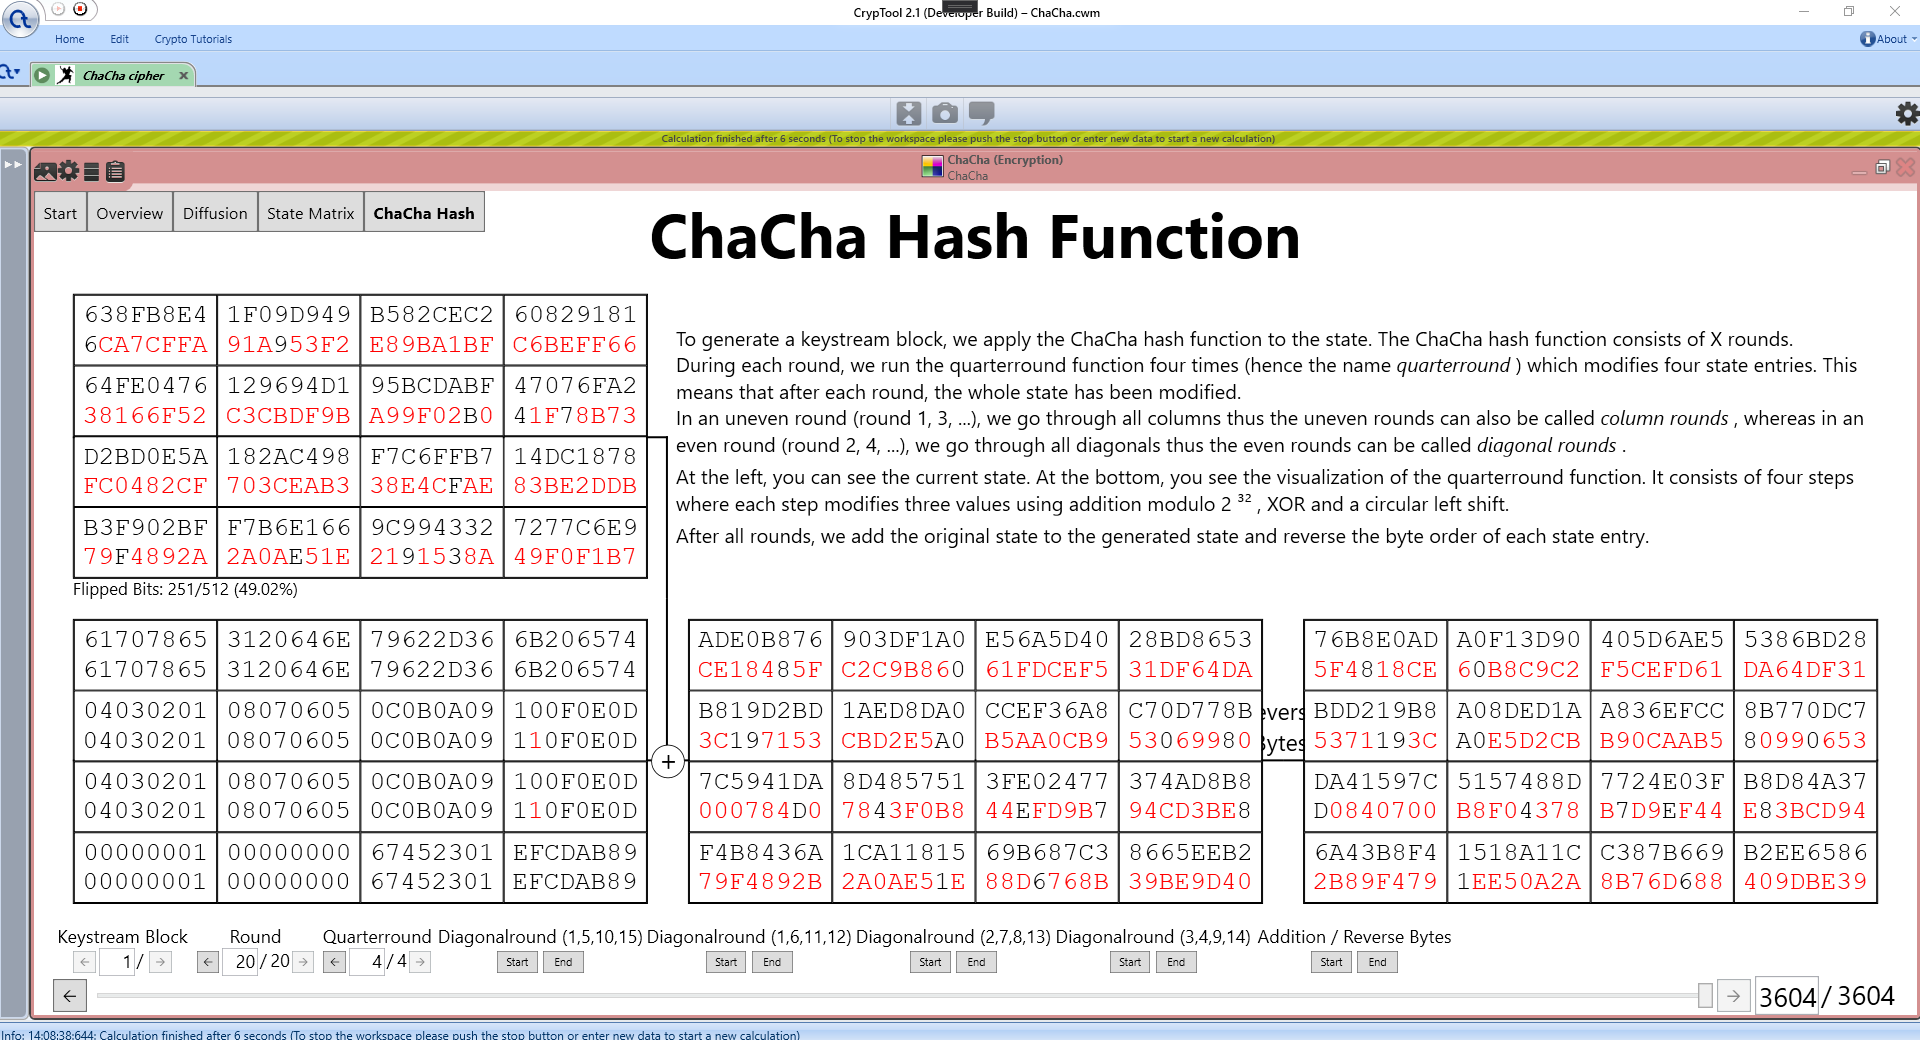
\includegraphics[width=\textwidth]{figures/ct2/chachahash/chachahash-end-diffusion.png}
  \caption{Addition and Little-Endian step visualization (with diffusion)}
  \label{fig:chachahash.end.with.diffusion}
\end{subfigure}
\end{figure}

\begin{figure}
\caption{End of quarterround execution of each column round of an uneven round \\(here: round 1)}
\label{fig:chachahash.cr}
\centering
\begin{subfigure}{0.5\textwidth}
  \centering
  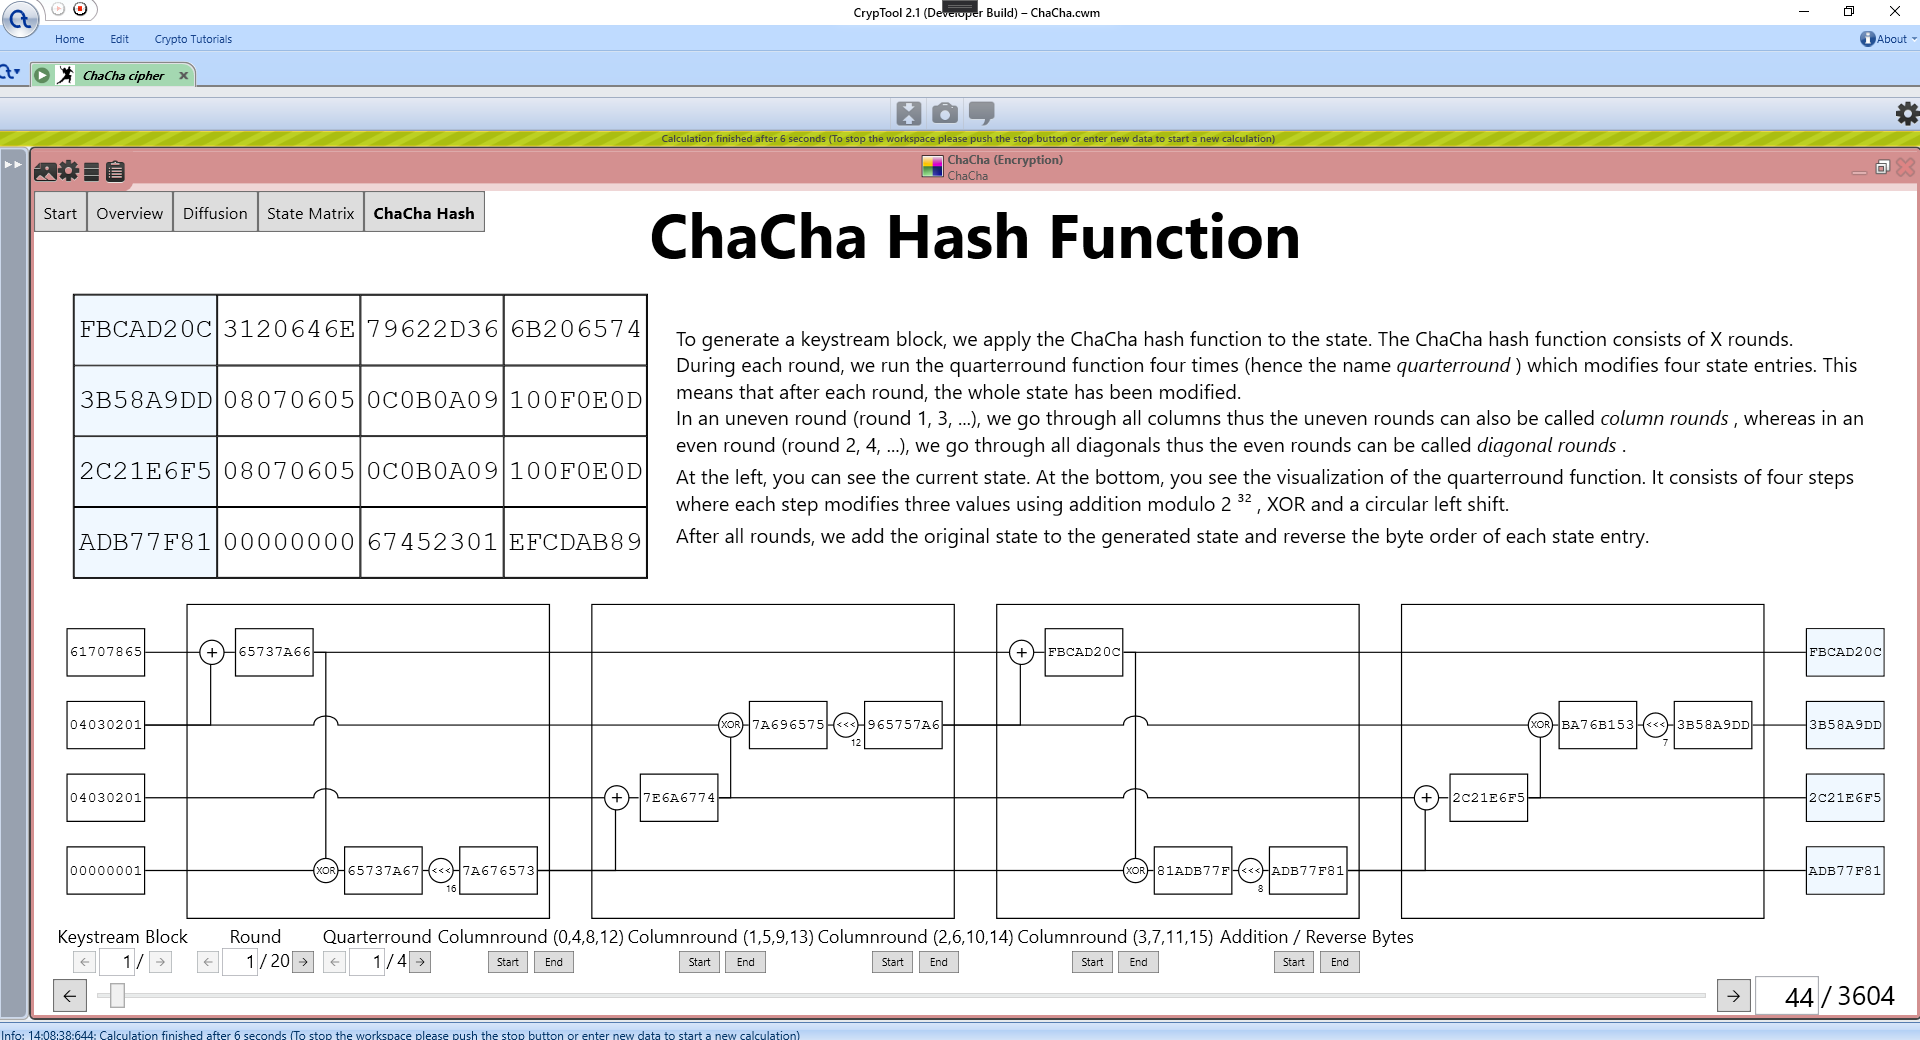
\includegraphics[width=0.99\textwidth]{figures/ct2/chachahash/chachahash-cr1-end.png}
  \caption{End of first column round}
  \label{fig:chachahash.cr.1}
\end{subfigure}%
\begin{subfigure}{0.5\textwidth}
  \centering
  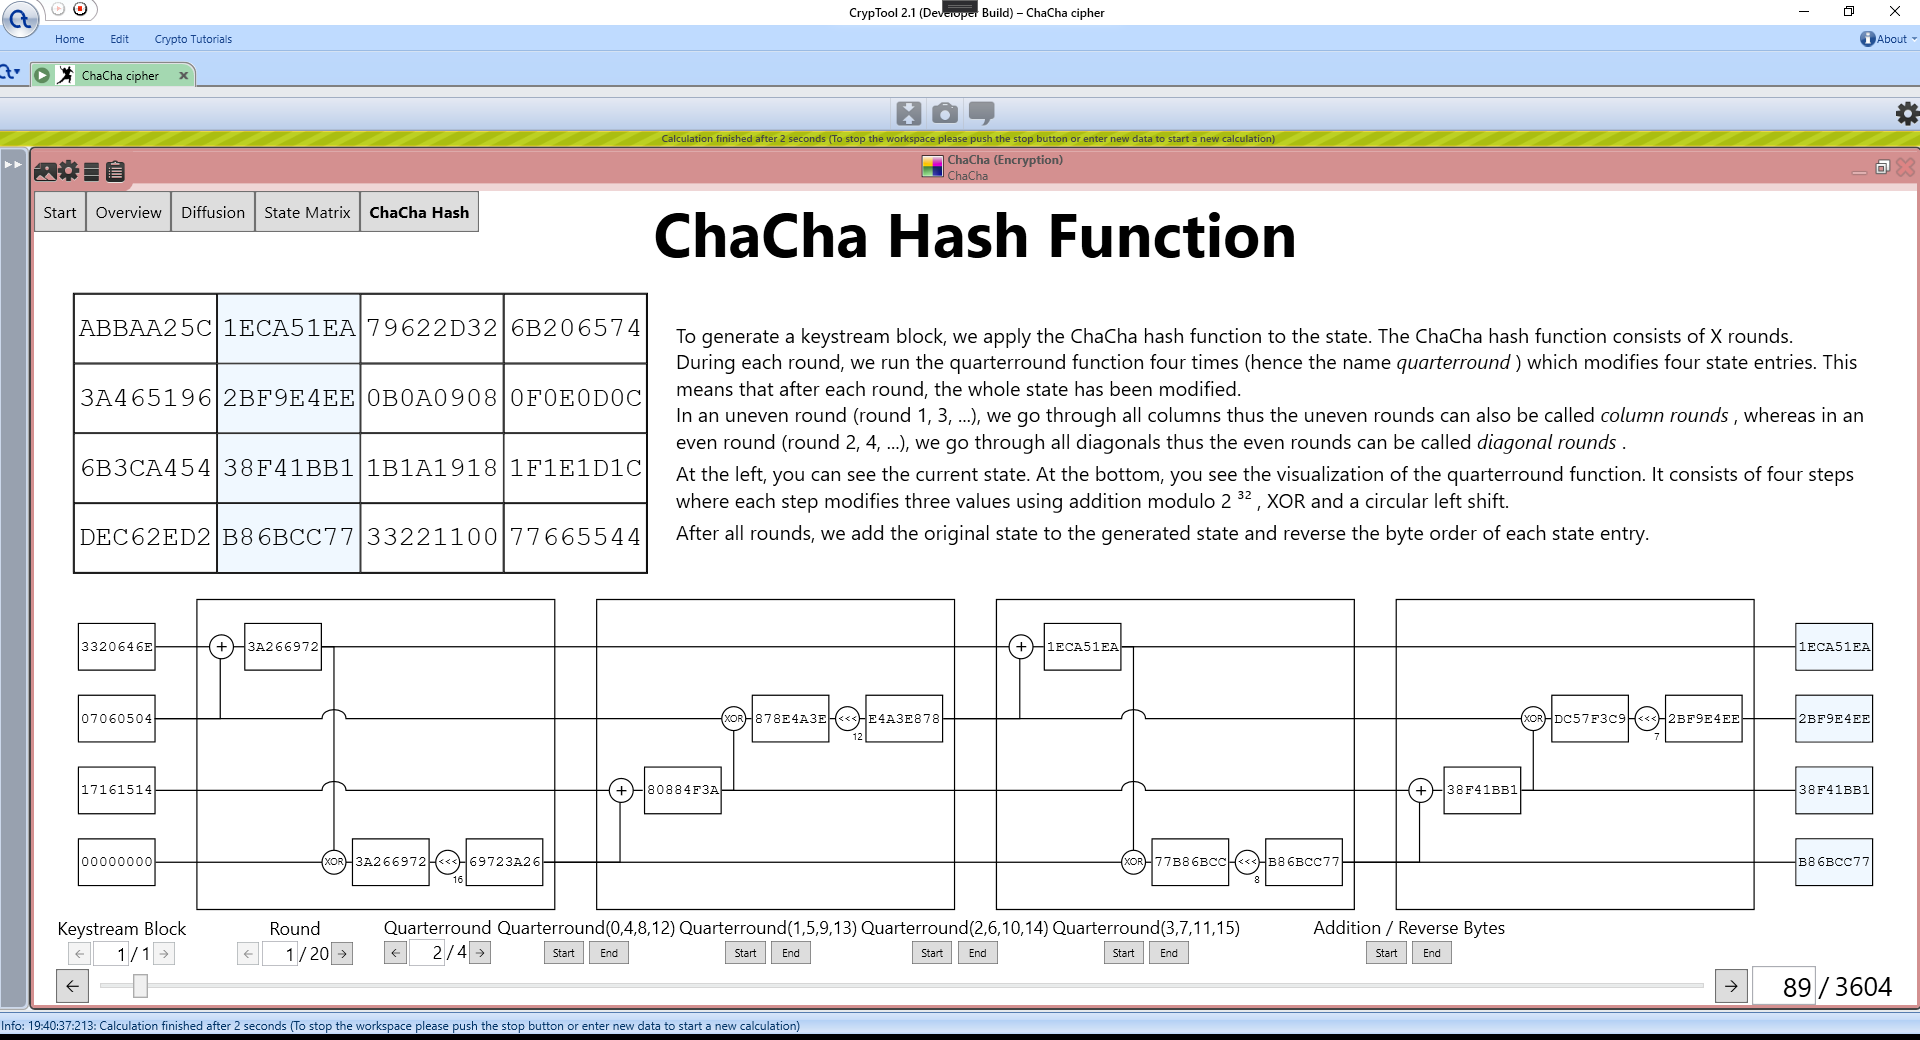
\includegraphics[width=0.99\textwidth]{figures/ct2/chachahash/chachahash-cr2-end.png}
  \caption{End of second column round}
  \label{fig:chachahash.cr.2}
\end{subfigure}
\begin{subfigure}{0.5\textwidth}
  \centering
  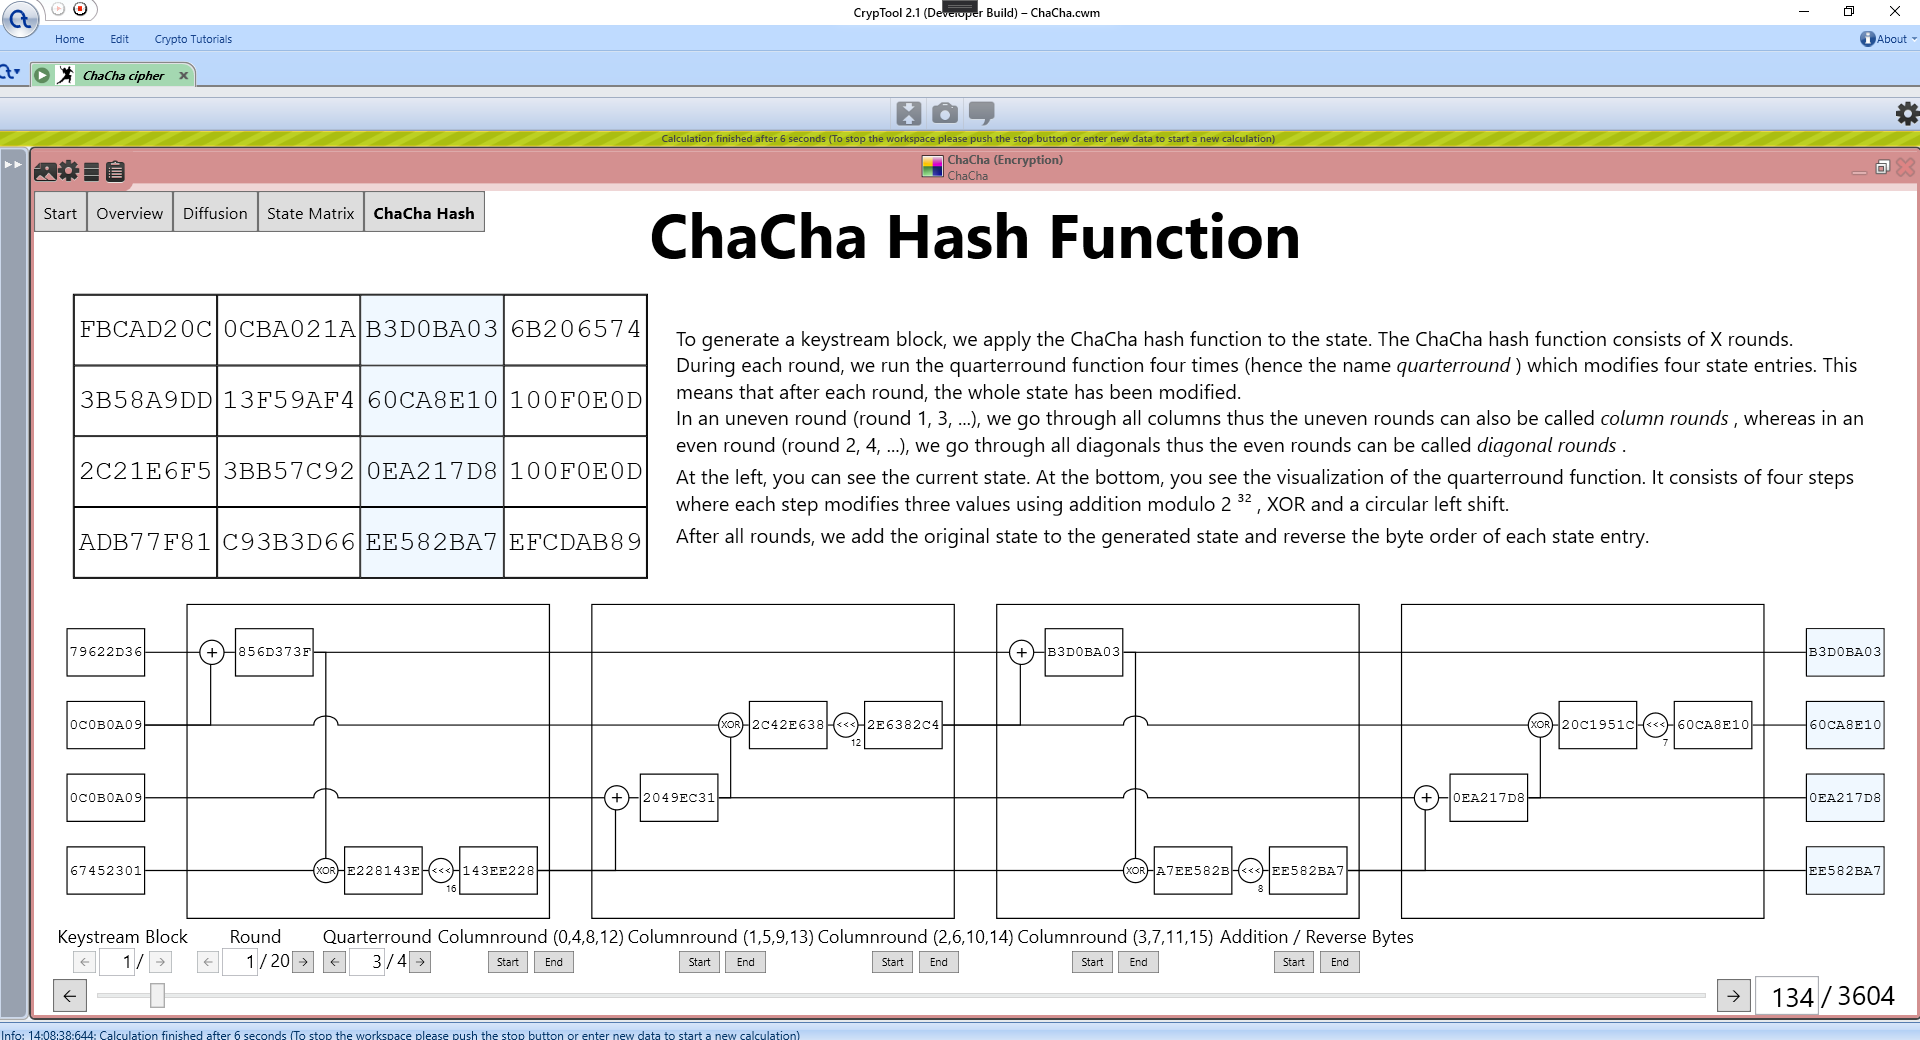
\includegraphics[width=0.99\textwidth]{figures/ct2/chachahash/chachahash-cr3-end.png}
  \caption{End of third column round}
  \label{fig:chachahash.cr.3}
\end{subfigure}%
\begin{subfigure}{0.5\textwidth}
  \centering
  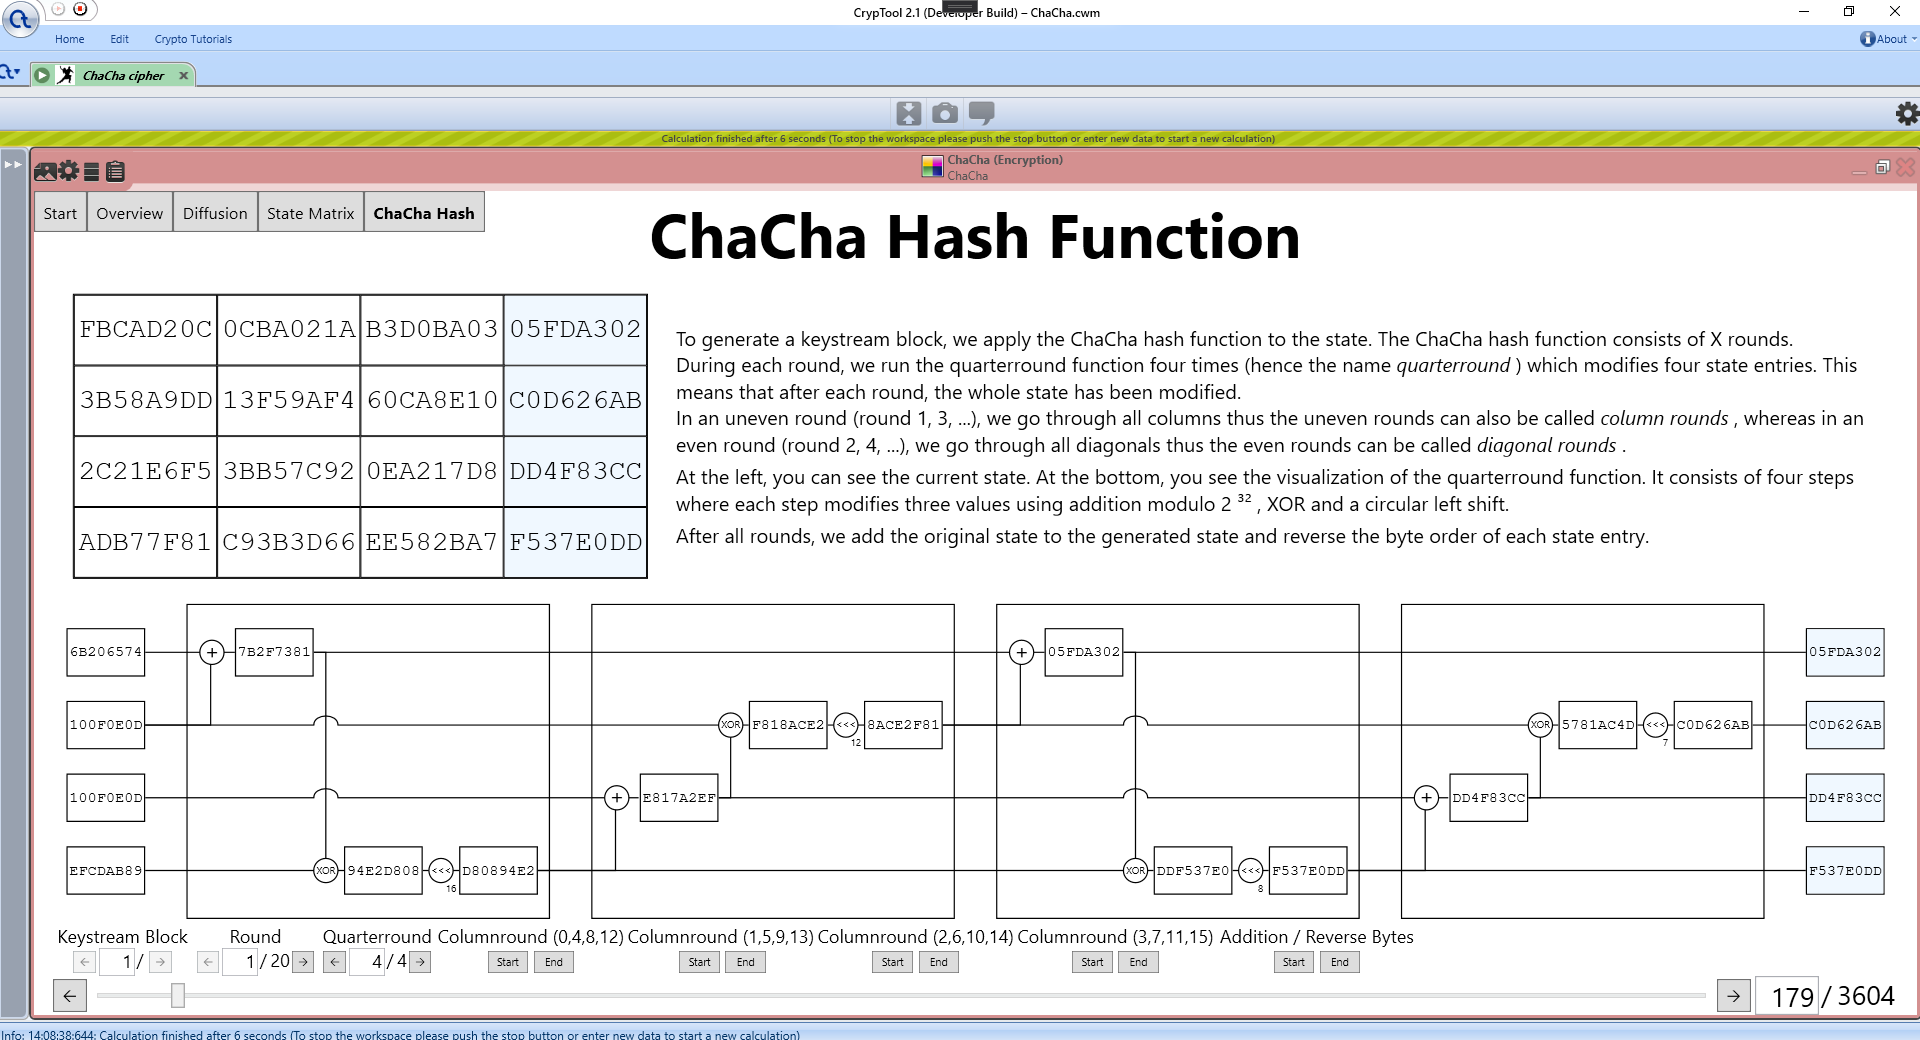
\includegraphics[width=0.99\textwidth]{figures/ct2/chachahash/chachahash-cr4-end.png}
  \caption{End of fourth column round}
  \label{fig:chachahash.cr.4}
\end{subfigure}

\caption{End of quarterround execution of each diagonal round of one even round \\(here: round 2)}
\label{fig:chachahash.dr}
\centering
\begin{subfigure}{0.5\textwidth}
  \centering
  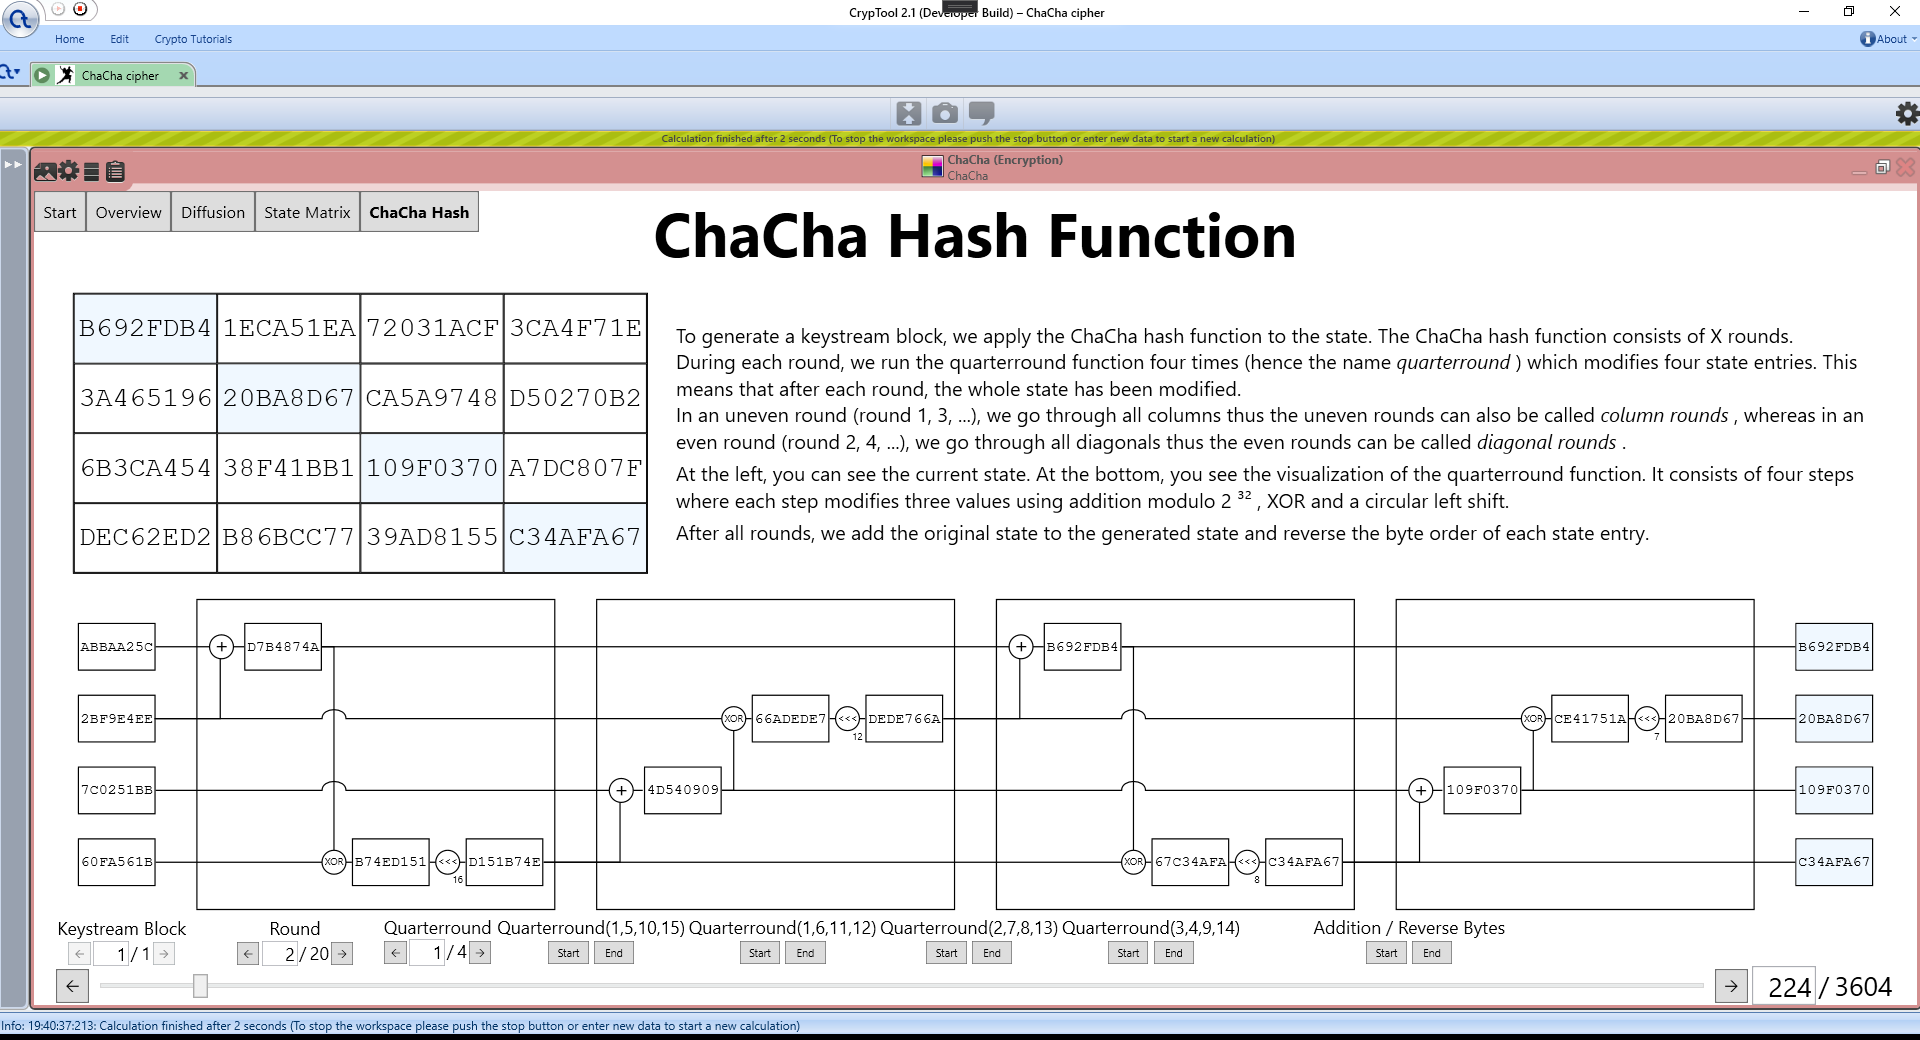
\includegraphics[width=0.99\textwidth]{figures/ct2/chachahash/chachahash-dr1-end.png}
  \caption{End of first diagonal round}
  \label{fig:chachahash.dr.1}
\end{subfigure}%
\begin{subfigure}{0.5\textwidth}
  \centering
  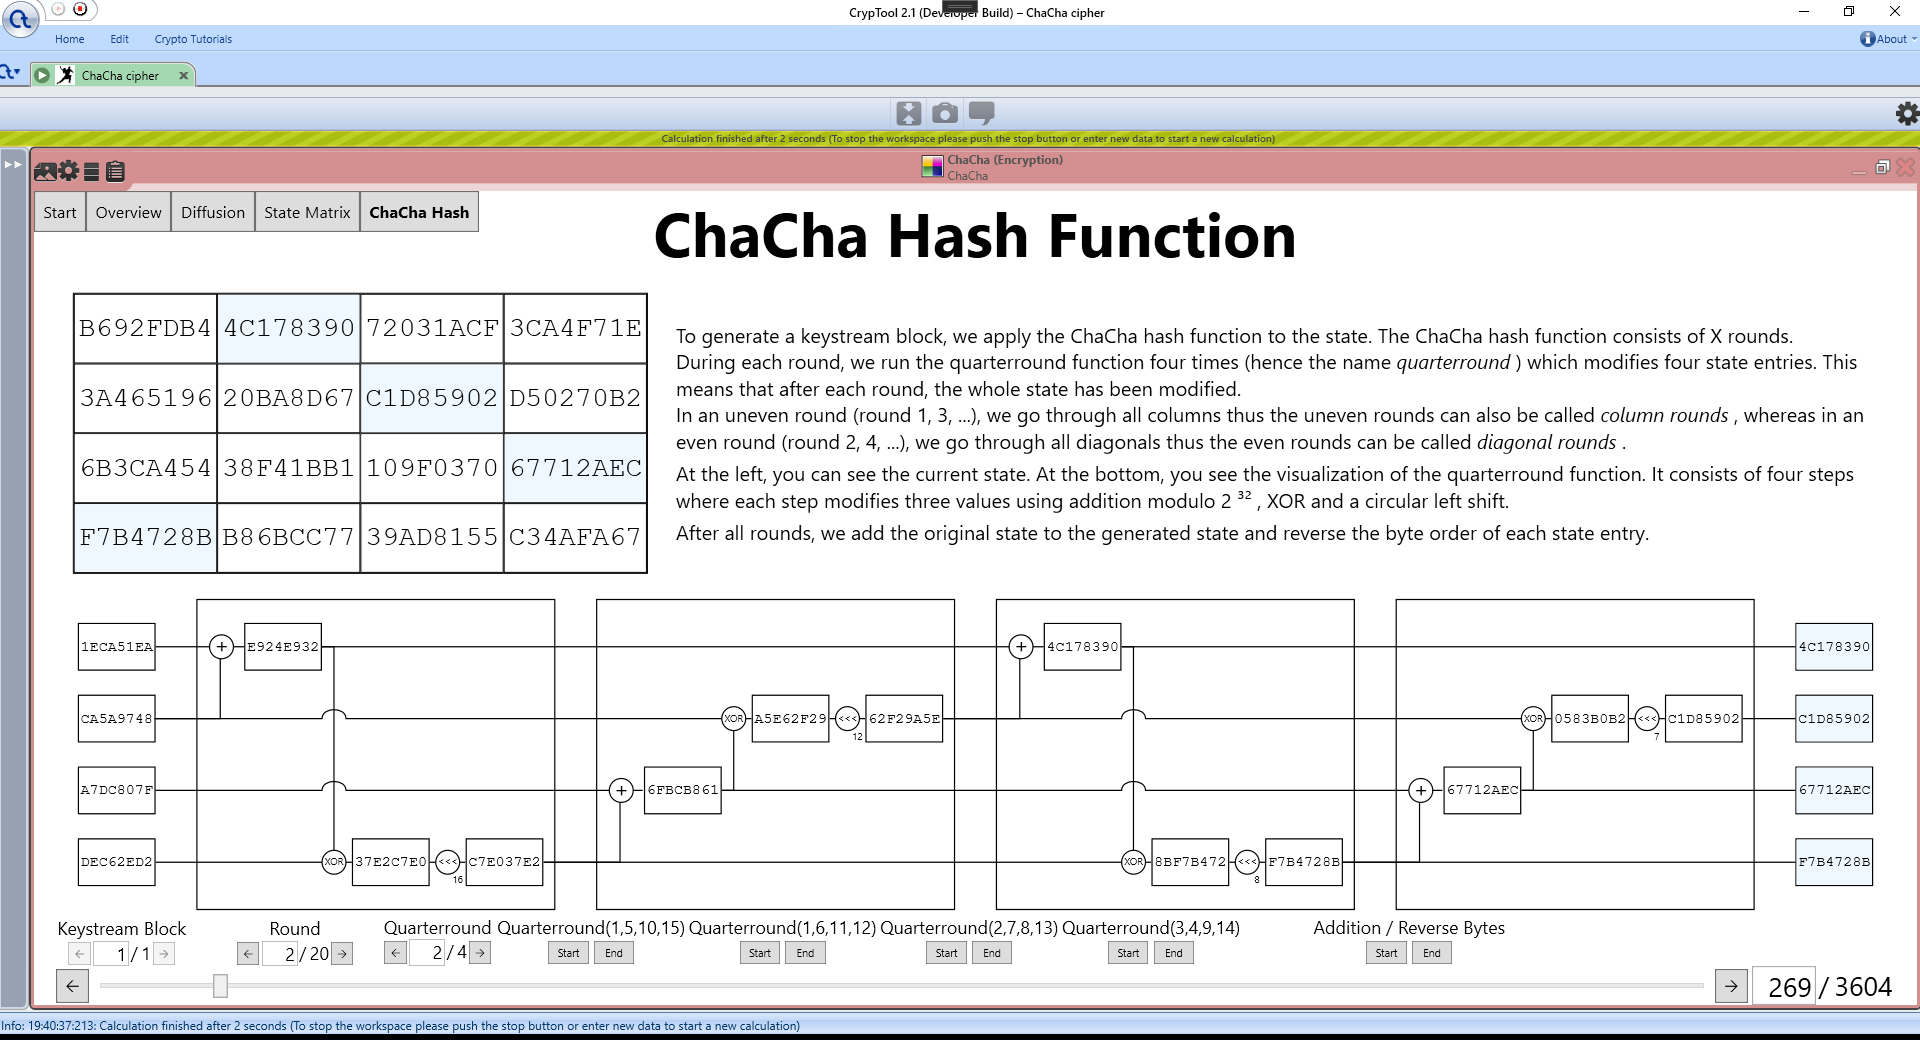
\includegraphics[width=0.99\textwidth]{figures/ct2/chachahash/chachahash-dr2-end.png}
  \caption{End of second diagonal round}
  \label{fig:chachahash.dr.2}
\end{subfigure}
\begin{subfigure}{0.5\textwidth}
  \centering
  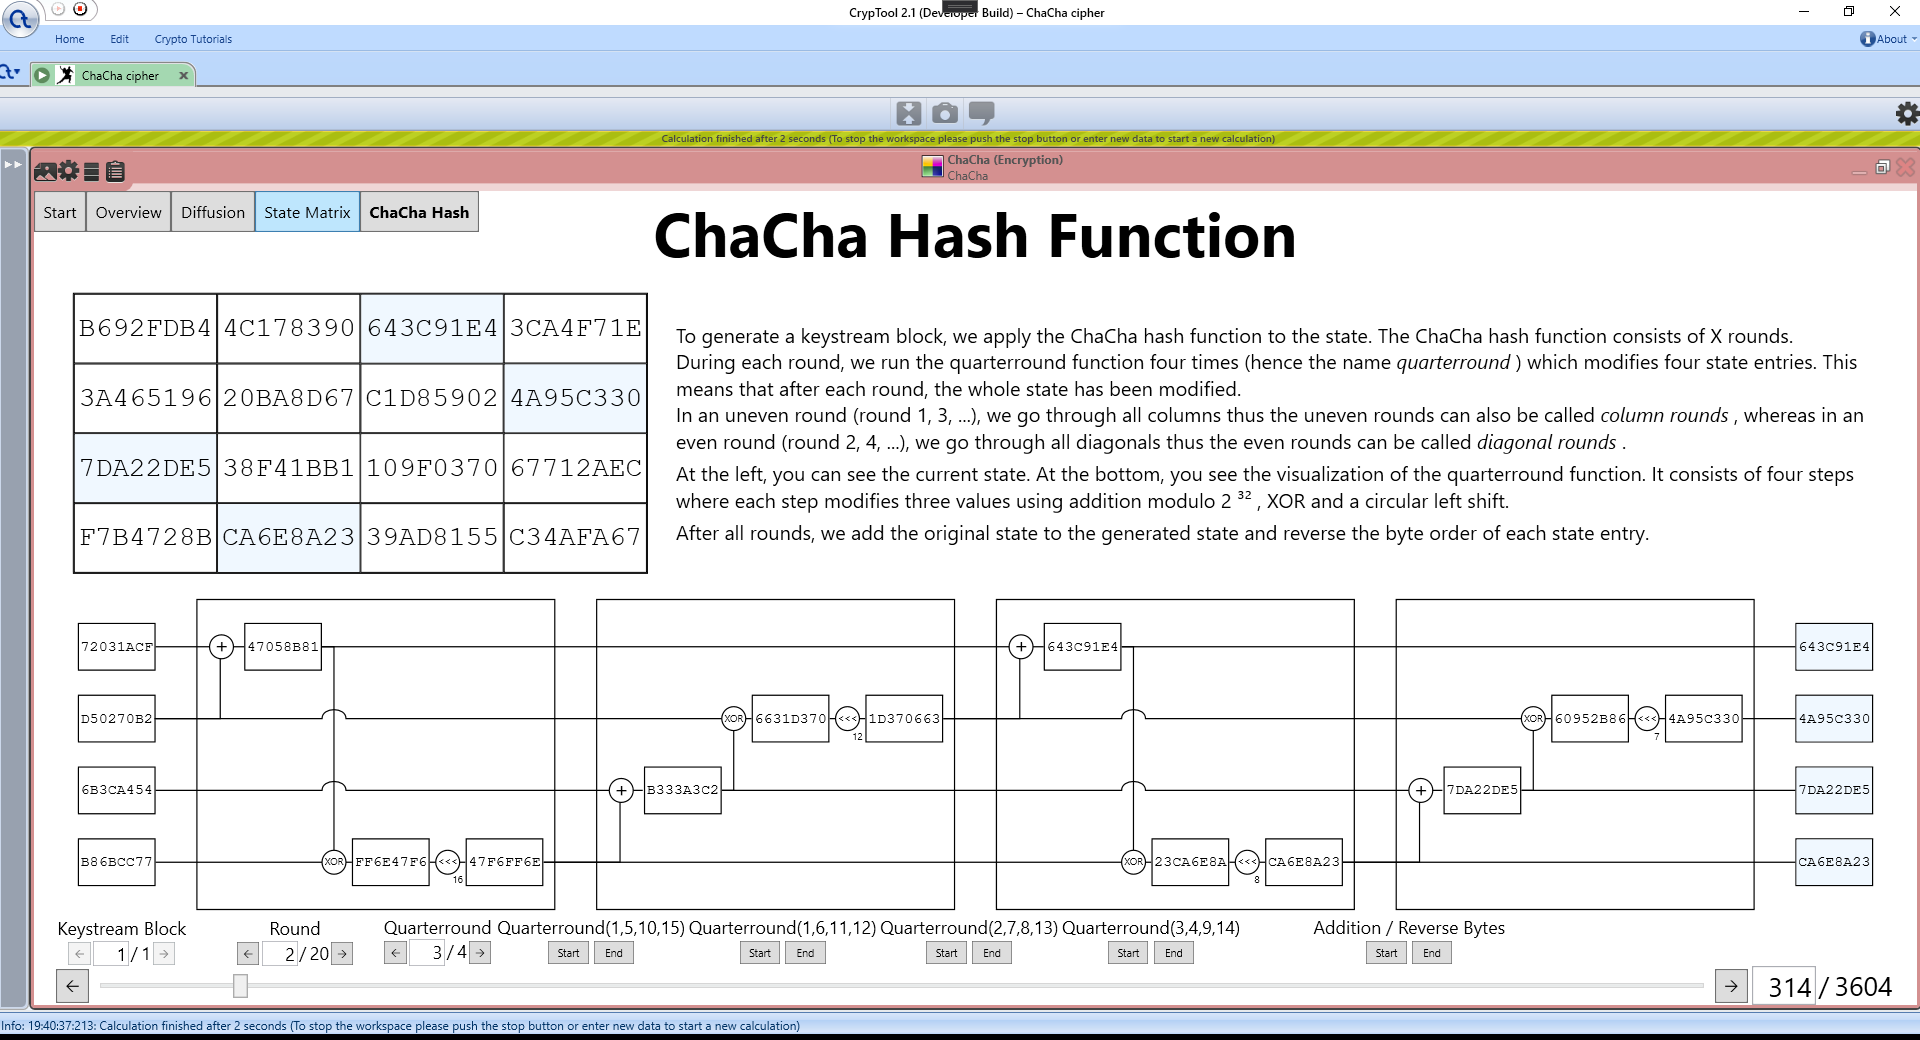
\includegraphics[width=0.99\textwidth]{figures/ct2/chachahash/chachahash-dr3-end.png}
  \caption{End of third diagonal round}
  \label{fig:chachahash.dr.3}
\end{subfigure}%
\begin{subfigure}{0.5\textwidth}
  \centering
  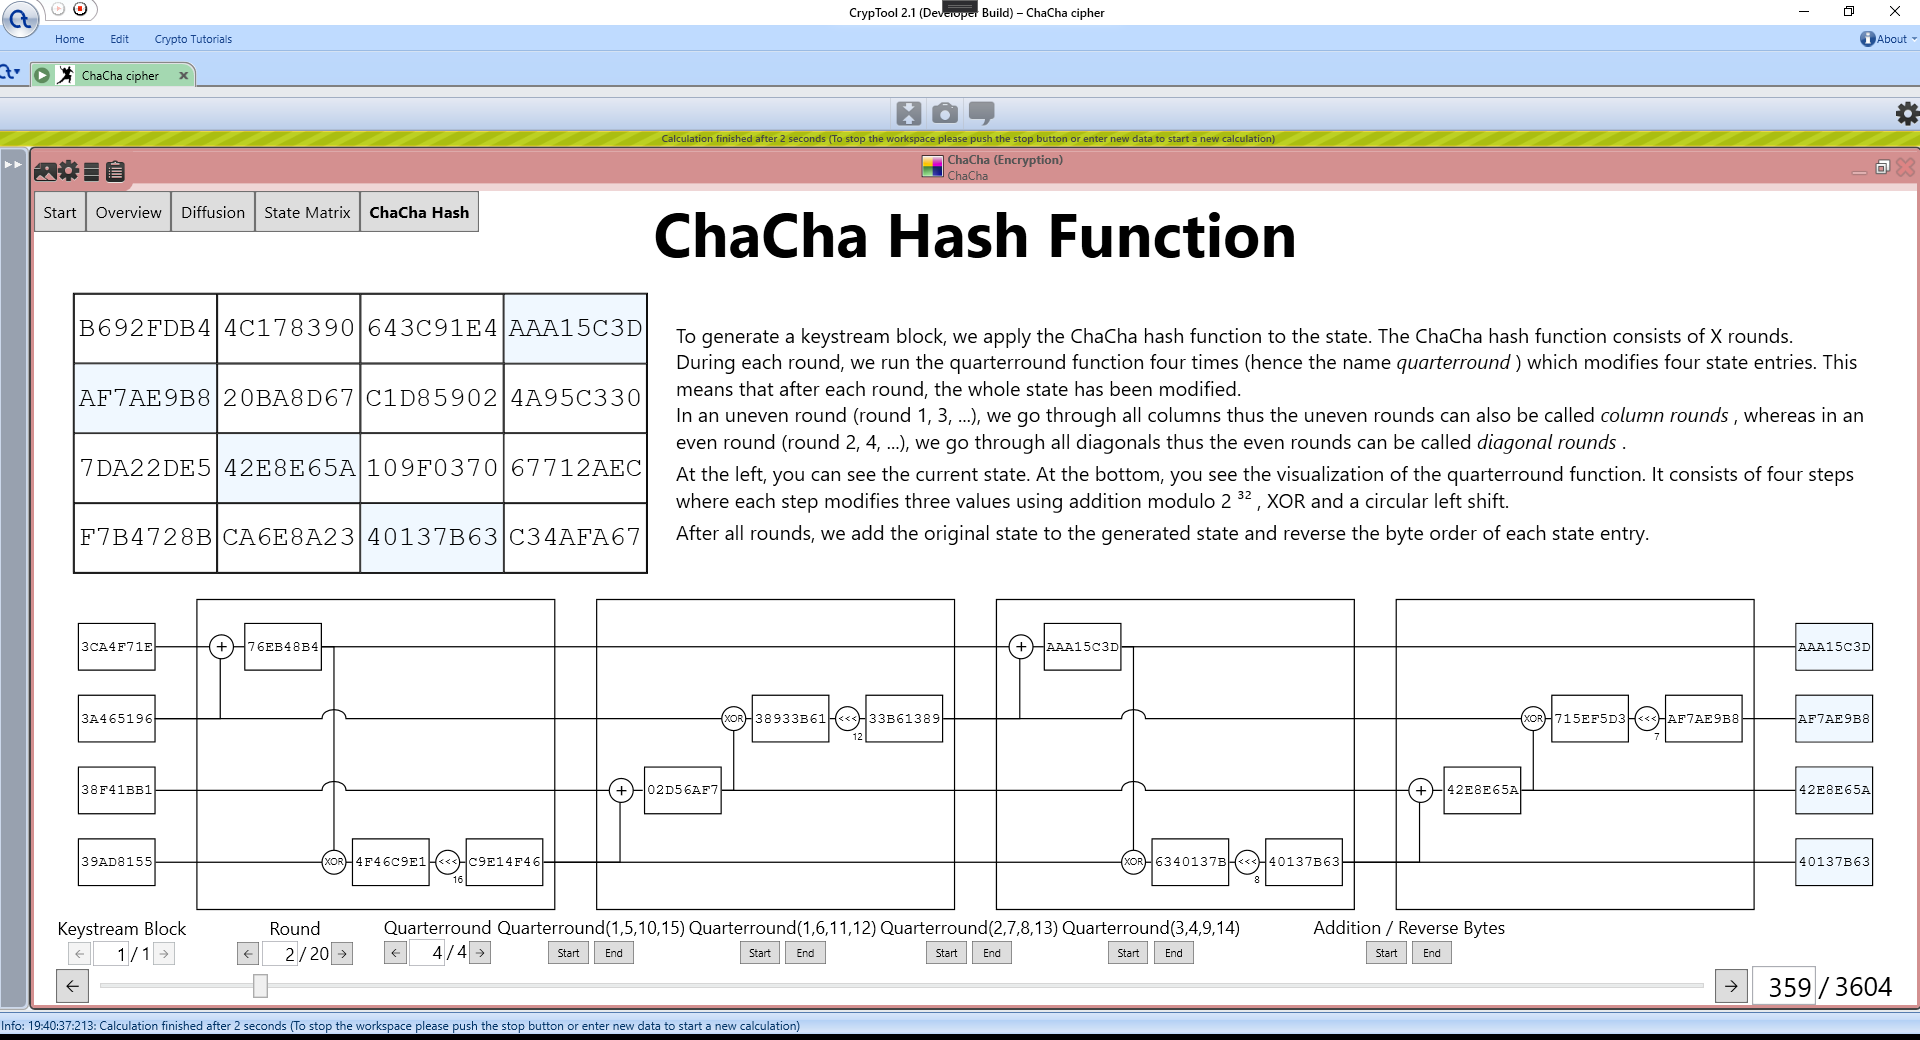
\includegraphics[width=0.99\textwidth]{figures/ct2/chachahash/chachahash-dr4-end.png}
  \caption{End of fourth diagonal round}
  \label{fig:chachahash.dr.4}
\end{subfigure}
\end{figure}

\subsection{Architecture}
\label{sec:Architecture}

In this section I will go more into detail how the software was layed out.

The software architecture, which was written using WPF (Windows Presentation Foundation), XAML and C\#7.0, can be split into two parts.

The first part is about the MVVM (Model-View-ViewModel) architecture to create the user interface which was explained in the previous section.

The second part is about the action navigation system which plays a huge role regarding performance. It powers the slider and buttons in the bottom row of each page. The page navigation is handled by the first part because it is very simple and uses MVVM design patterns. \\
I have named the action navigation system \textit{\textbf{centralized navigation system}} for reasons I will explain in its subsection.

\subsubsection{MVVM architecture}

I have used a MVVM architecture because in previous attempts, I have discovered that without following a design pattern with its standards and rules, the code becomes complicated over time; making it harder to fix bugs or implement new features. \\
Even though I tried to follow some self-chosen guidelines like naming conventions and which code should go where, most of the time I went the path of least effort to have results as fast as possible which I could showcase to my supervisors and ask for feedback. The internal code structure was of no importance as long as the feature worked. Only when I realized that it got too cumbersome to maintain this workflow, I read about using design patterns in WPF applications and found out that MVVM is the most popular design pattern to use in conjuction with WPF \cite{mvvm-wpf}.

As the name suggest, MVVM is all about separating the code into three parts: Model, View and the View Model.

Models hold the raw application data. In our case, this would be the classes which hold the values generated by the ChaCha cipher. It should be completely unaware of any View or ViewModels.

Views define how the data should be presented. They consist mainly of XAML code with as little code-behind as possible. They do not maintain their own state but rather use data binding to synchronize themselves with the data inside the ViewModels. Therefore, it is aware of the existence of ViewModels.

ViewModels connect the model data with the views. However, they do not directly manipulate the views but just define properties and methods to which the views can attach themselves to implement the logic for user interactions. For example, a ViewModel implements the page navigation and saves the user input on the Diffusion page to execute the cipher with these values on page exit. It does not define how the buttons or text inputs should look like.

In Figure \ref{fig:mvvm.pagenavigation}, I have provided an example for how this data binding looks in code. What you see is the view code for the page navigation.

Another technique (that you can also see in the mentioned Figure) is the use of templates. I have used data templates to attach views to viewmodels and control templates to implement the general UI structure with the three sections I mentioned in Section \ref{sec:userInterface}. This enabled me to define the UI layout for all pages in one place and also reuse a single implementation of the page and action navigation across all pages. This way, modifications down the road which applied to all pages were easy and fast. \\ In Figure \ref{fig:mvvm.actionnavigation}, you can see the view implementation of the action navigation bar which is only visible on pages which do have actions.

\begin{figure}
\caption{Implementation of page navigation using data binding}
\label{fig:mvvm.pagenavigation}
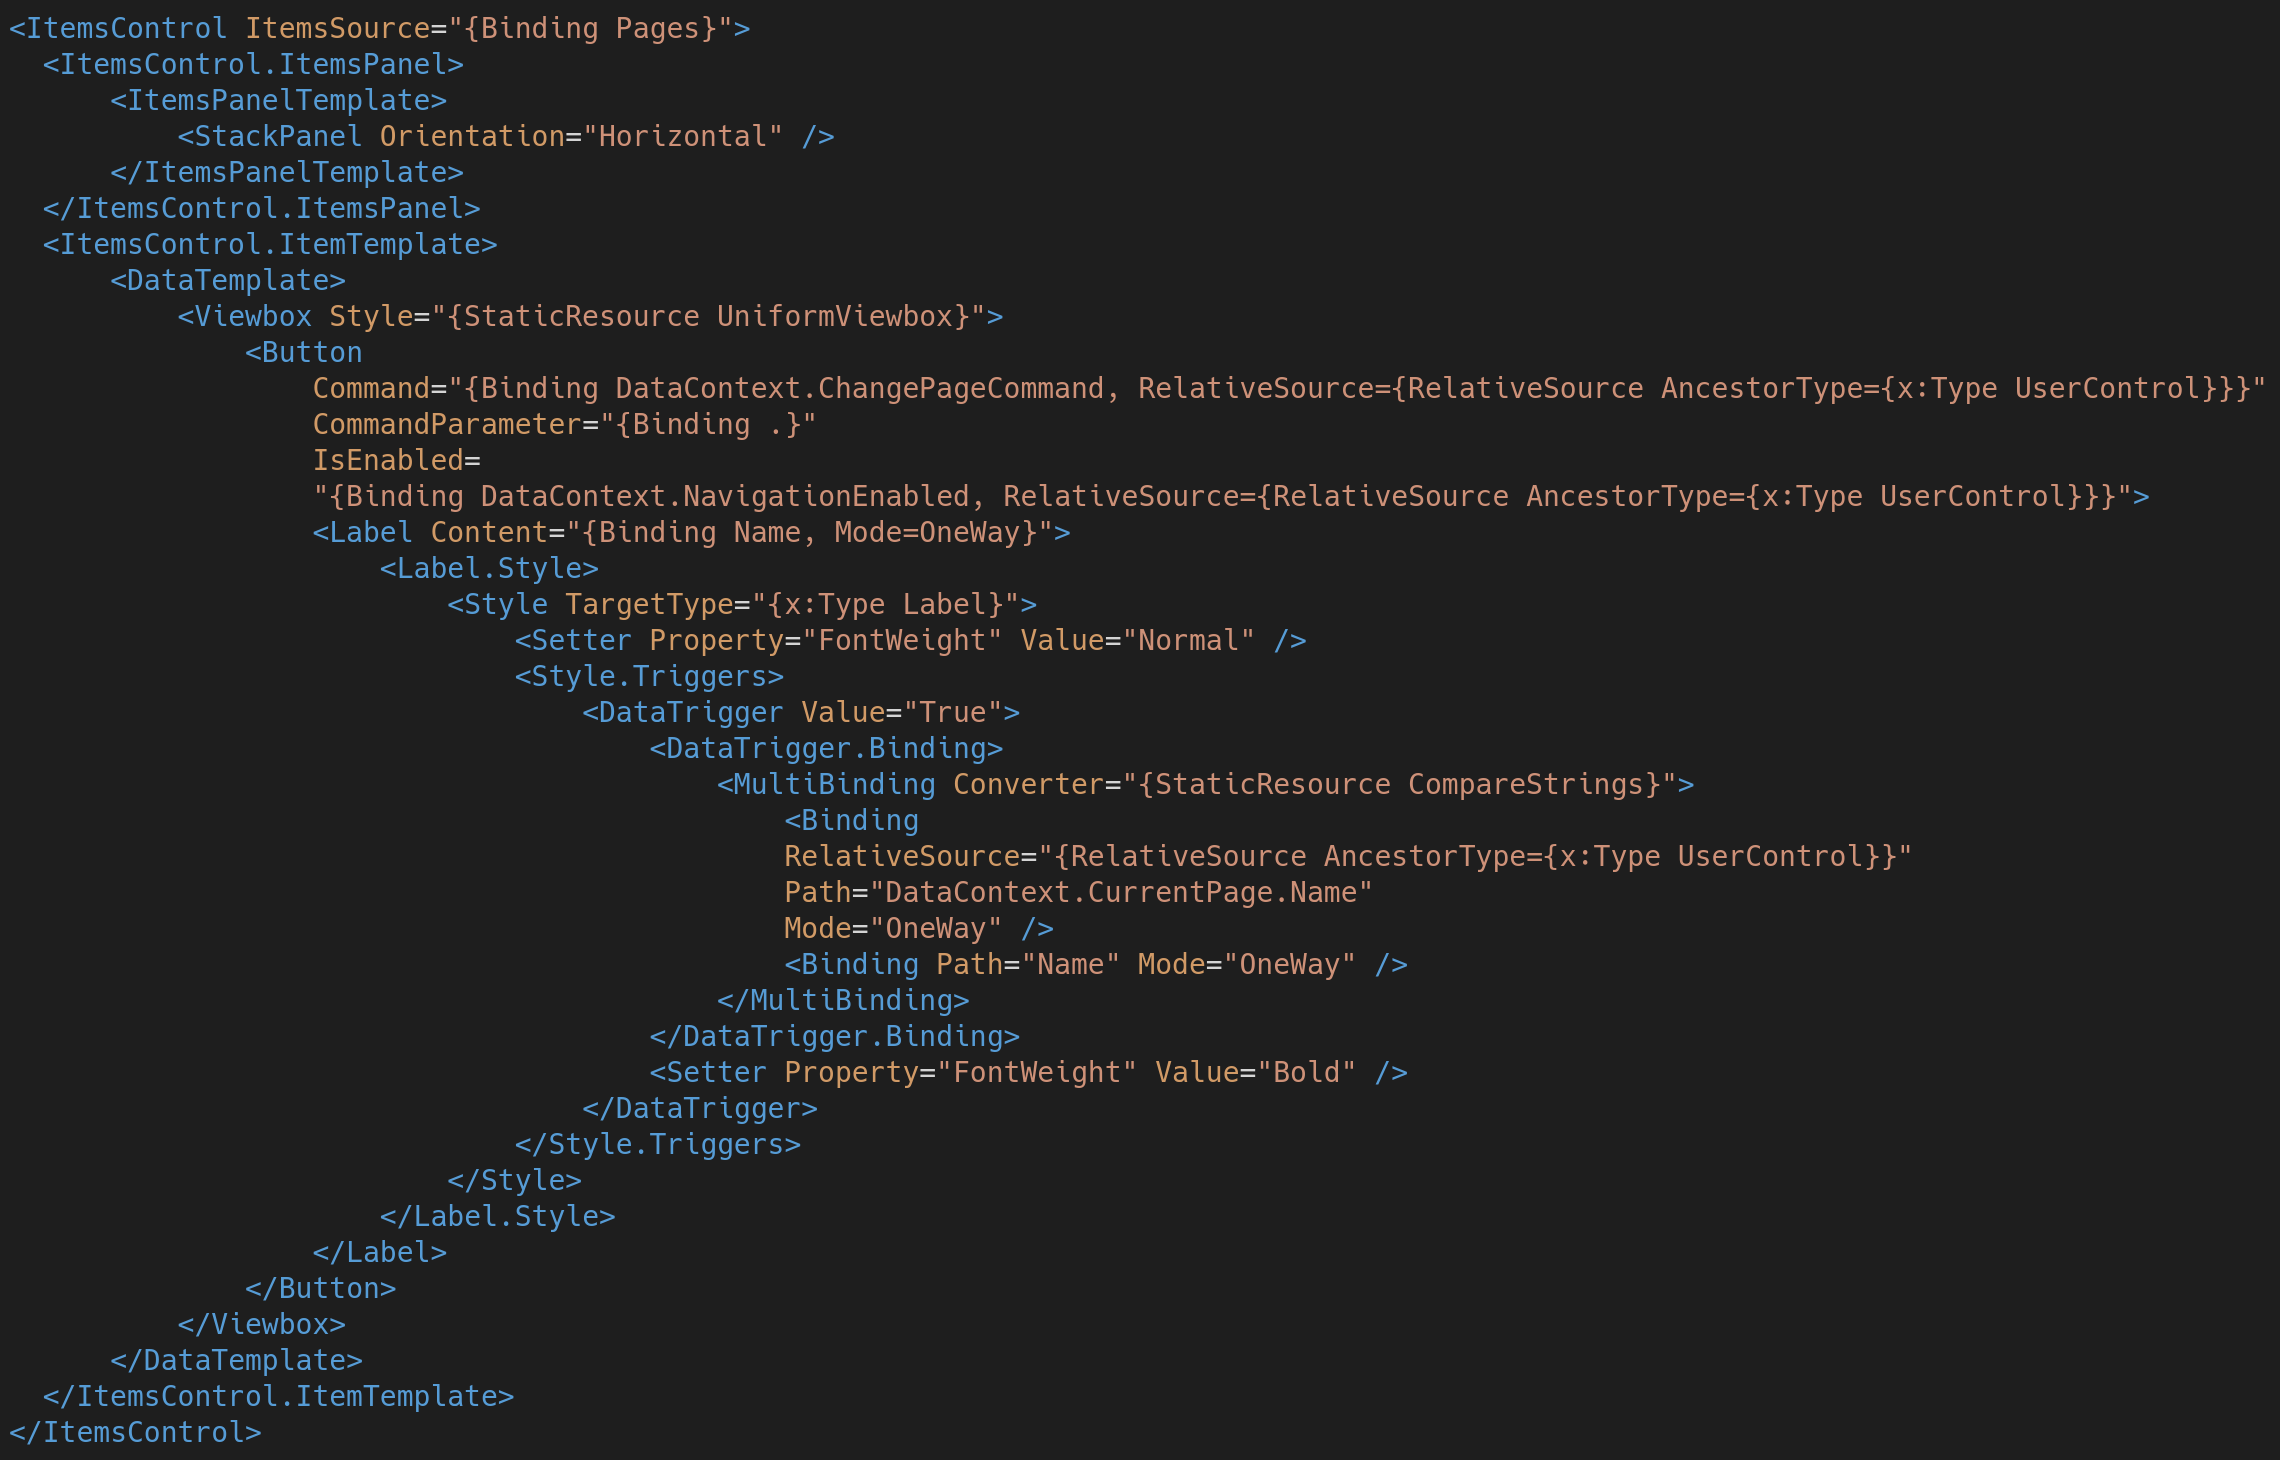
\includegraphics[width=\textwidth]{figures/code/mvvm-arch/page-navigation-template.png}
\caption{Implementation of action navigation inside a control template}
\label{fig:mvvm.actionnavigation}
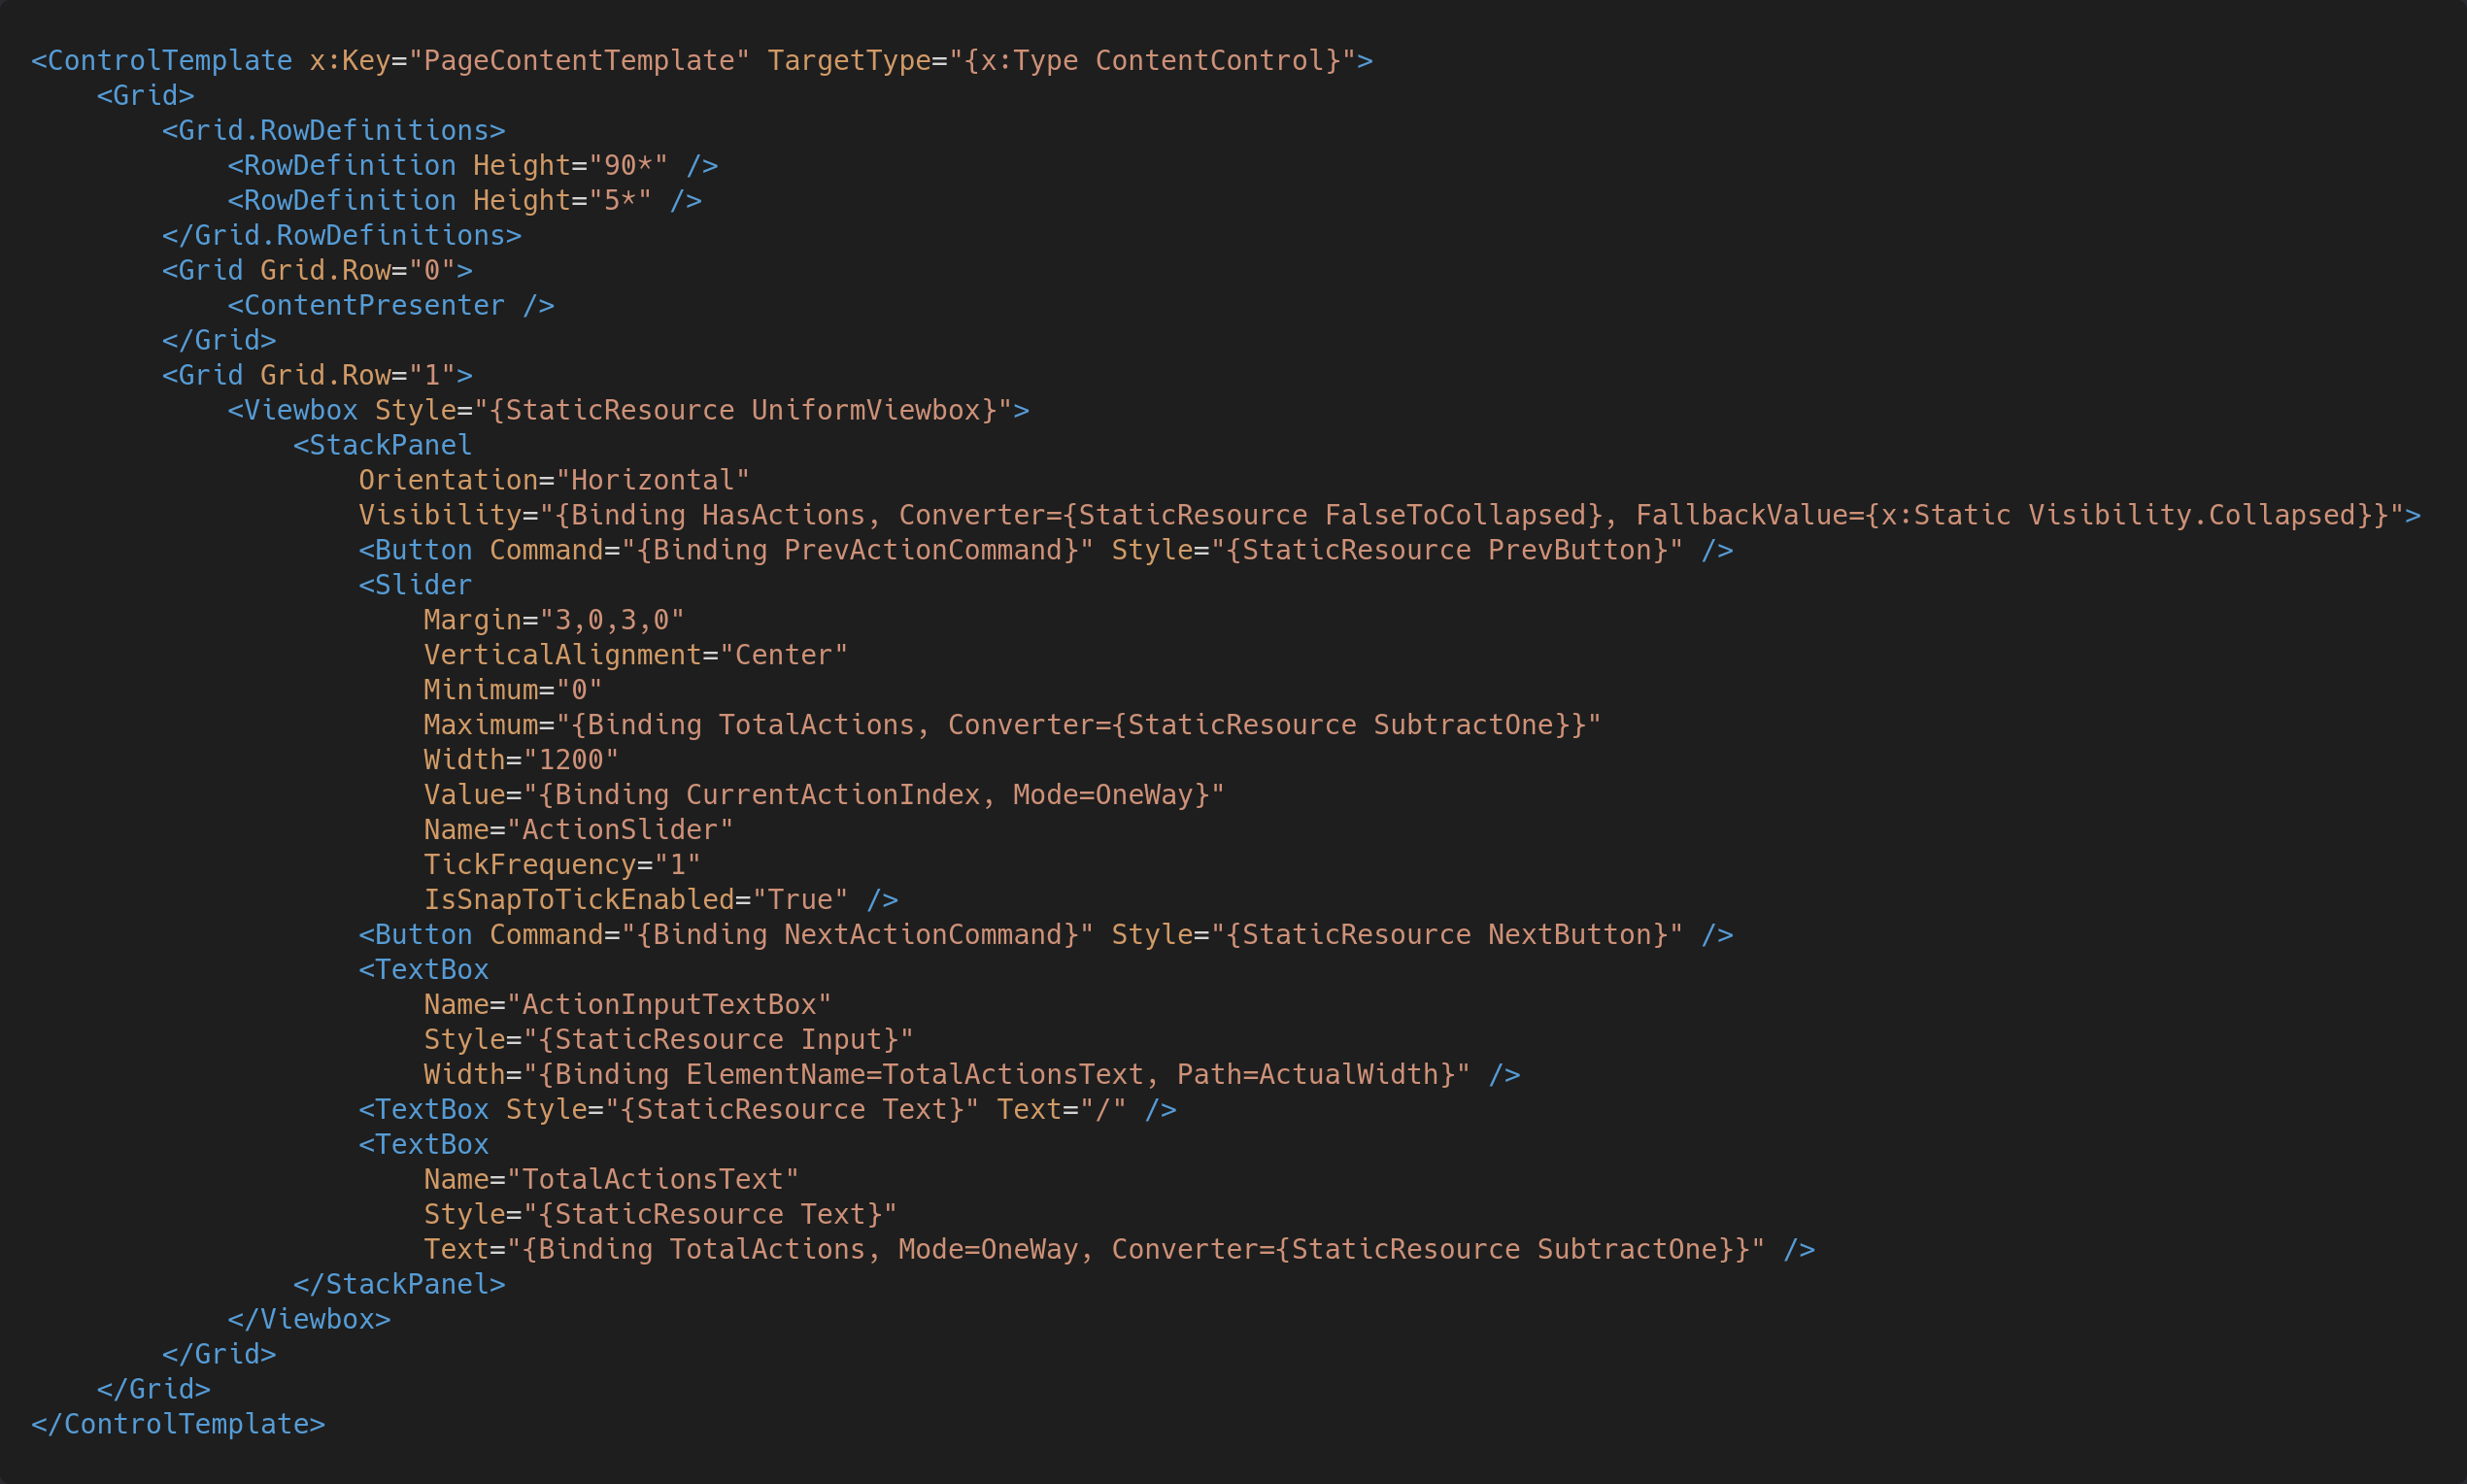
\includegraphics[width=\textwidth]{figures/code/mvvm-arch/action-navigation-template.png}
\end{figure}

Since the most interesting part about the MVVM architecture is probably how the diffusion visualization works, I will explain this feature in more detail.

If the user enters something into the input fields for the secondary values, validation of the input occurs. It checks if the input contains only valid hexadecimal characters and if the size is not too large. This is done by extending the \texttt{ValidationRule} class which is a built-in module of WPF. Only if the input is valid, the value is saved into a property of the underlying view model. This way, we can be sure that we always have a sane data with which we later can execute the cipher with. Since data binding works by notifying the view if a variable has changed. WPF provides an interface named \texttt{INotifyPropertyChanged} which helps with implementing these data binding notifications. It provides a method named \texttt{OnPropertyChanged()}

\begin{figure}
\centering
\caption{Data binding notification implementation}
\begin{subfigure}[t]{0.5\textwidth}
\caption{Data binding notification in setter of \texttt{DiffusionInputKey}}
\label{fig:mvvm.onpropertychanged}
\centering
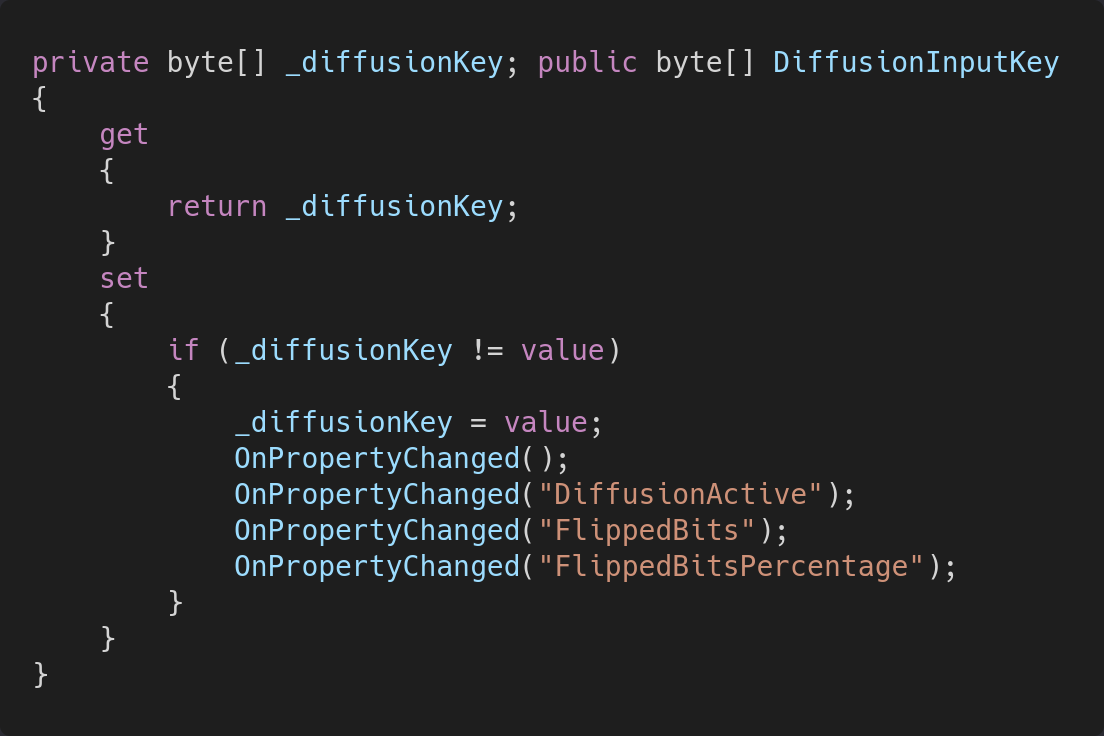
\includegraphics[width=0.99\textwidth]{figures/code/mvvm-arch/onpropertychanged.png}
\end{subfigure}%
\begin{subfigure}[t]{0.5\textwidth}
\caption{\texttt{ViewModelBase} implementation with \texttt{INotifyPropertyChanged} interface}
\label{fig:mvvm.viewmodelbase}
\centering
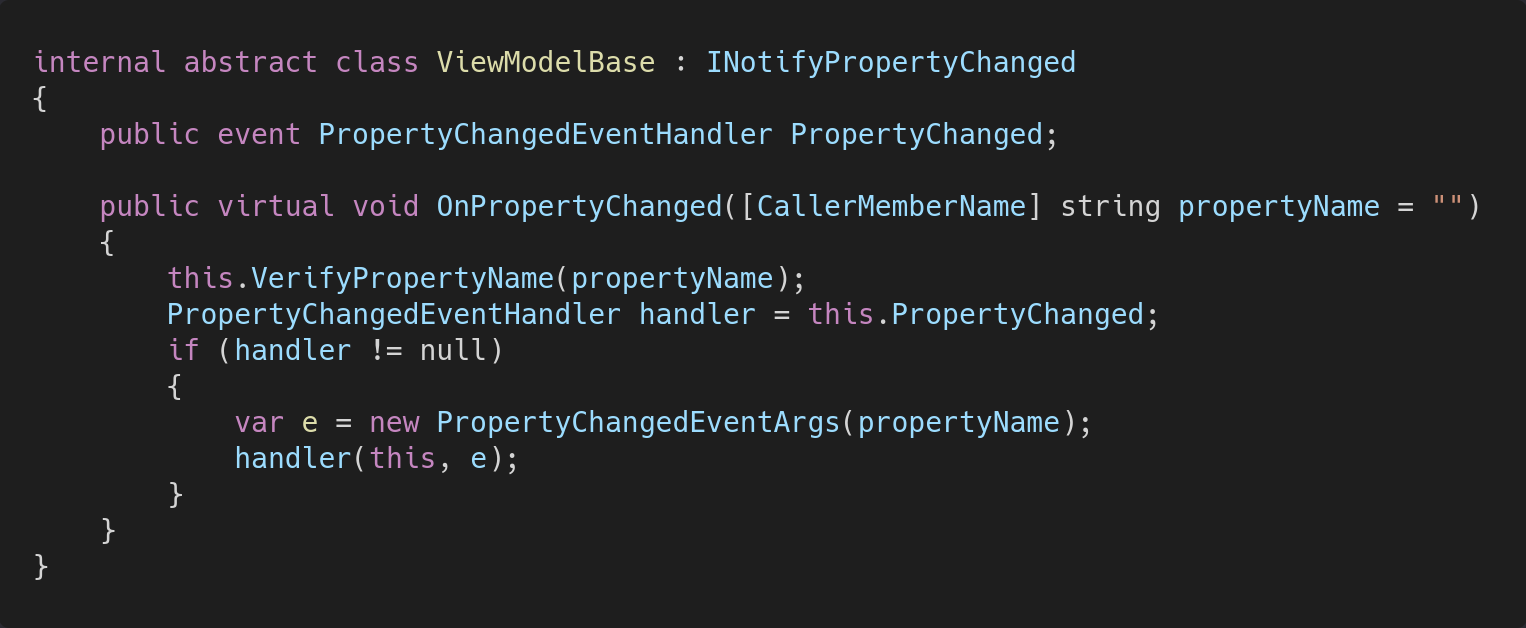
\includegraphics[width=0.99\textwidth]{figures/code/mvvm-arch/viewmodelbase.png}
\end{subfigure}
\end{figure}

\subsubsection{Centralized navigation system}



%%%%%%%%%%%%%%%%%%%%%%%%%%%%%%%%%%%%%%%%%%%%%%%%%%%%%%%%%%%%%%%%%%%%%%%%

\section{Encountered Problems}
\label{sec:encounteredProblems}

In this section, I will discuss the main problems I encountered during implementation. To briefly summarize, they mainly consisted of how to create a simple, intuitive user interface and how the system behind the interface should be designed to have the best or at least a reasonable performance. \\
In the other visualizations, I noticed that I was quite overwhelmed by the amount of buttons which were visible, even though not always enabled. So I wanted to keep my user interface as simple as possible while not restricting the user in his ability to navigate through the visualization. \\
Regarding the performance, the author of the AES visualization has mentioned in his thesis that to create a fluent user experience where he can navigate back and forth between all steps, the intermediate values need to be calculated beforehand and saved since we don't want to stop at each step to calculate the next value or recalculate everything from the start if the user wants to go backwards. I came to the same conclusion. But as I will describe on the next pages, this was not all that was needed to ensure such an experience.\\
I hope that the description of these problems and the solutions I have found may help future students in writing their own plugins.

\subsection{Architecture}

\subsubsection{Linear navigation system}

The peformance of the plugin was essentially coupled to how the navigation system was designed. Other things like the aforementioned calculation of the intermediate values for the visualization were compared to the navigation system design unsignificant because they are created by the ChaCha cipher anyway and must just be saved somewhere to not lose them. This means that storing them was only a necessary but not sufficient condition for a overall good performance. \\
I realized this early in development when I had my first page with many page actions on it and wanted to skip ahead a lot of actions. While implementing this feature which would enable the user to skip from any action to any other action, I realized that when skipping more than 100 actions, it already took about 750ms during which the UI was unresponsive. As can be seen in Figure \ref{fig:navsystem.linear.stats}, this time increased linearly so it was quite clear that I needed to do something about this, especially because the page with the most actions had over 3000 single actions.

The root cause of the problem was the navigation system design which I called in hindsight \textbf{\textit{linear navigation system}}. It consisted of defining actions which build upon each other. This means that if we are at action 0 (initial state of the page) and want to go to action 5, we need to execute all the code inside the action definitions between 0 and 5 to arrive at the page state as it should be at action 5. This is resembled in Figure \ref{fig:navsystem.linear.overview}. \\
I came up with this design to have a smooth implementation experience where I only have to write the actual page state changes between two actions instead of duplicating a lot of code since the page state changes which were applied during a previous page were most of the times still visible when moving to the next action. This complements how the user experiences the visualization because the actions are numbered in a sequence and thus are inherently linear. Because of this, it made a lot of sense to me to reflect this in the system architecture.

Since this "design flaw" was not the leading cause of the performance problem (going through a for-loop of size 3000 does not directly lead to performance issues), I want to briefly explain how the actual action implementation looked like.\\
As can be seen in Figure \ref{fig:navsystem.linear.detail}, during the transition between two page states, the state of the page elements which will change is saved such that we can undo the changes if the user decides to navigate back. This enabled me to skip writing action definitions for backwards navigation, since I could just write a function which retrieves the state corresponding to the transition and then applies it. This function would then work for all backwards navigation without further intervention which was very convenient during development. \\
The problem with that architecture was that the state saving and the execution logic inside the action definitions were changing a lot of page elements directly by accessing them via their name that I gave them in the XAML code. That this was against best practices in writing WPF applications I only noticed later on, when I read more about them. This issue combined with the restricted, linear pathing between actions resulted in that huge performance loss that was described in Figure \ref{fig:navsystem.linear.stats}.

\begin{figure}
\caption{Navigation paths between actions in the linear navigation system}
\label{fig:navsystem.linear.overview}
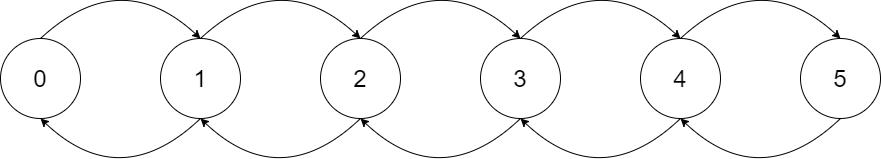
\includegraphics[width=\textwidth]{figures/navigationsystem-diagram/navigationsystem-linear-overview.png}
\end{figure}

\subsubsection{Linear navigation system with caches}

After identifying the two underlying issues, I implemented what I called a \textbf{\textit{linear navigation system with caches}}. As the name suggests, I implemented cache entries to be able to navigate in constant time between an action and an action for which I created a cache. To not only increase peformance during these transitions but between all transitions, we check before each transition, if first moving to a cached entry would decrease the amount of hops needed to go to our destination. \\
The cache entries consisted of instructions to restore the complete state of a page at the action index for which this cache entry was for. They contained instructions for the complete state instead of only the difference between two actions because now, moving to that cache must initialize the page, independent at which action / page state we were before. This means that there was some overhead in initializing the page because essentially, I cleared the whole page and then initialized the page elements with their appropriate content, potentially leading to some unnecessary code execution because the content prior to cleaning was already the one we needed. But this overhead was . Figure \ref{fig:navsystem.cache.overview} demonstrates that the navigation system now needs less hops between any two given actions. This increased performance significantly as can be seen in \ref{fig:navsystem.cache.stats}.

Further, to decrease the load on the CPU while dragging the action slider, I implemented a very simple asynchronous navigation. It was implemented by using a stack as a buffer for the values received from the slider during dragging. Every 50ms, the last value from the buffer is read and the page moves to that action. Afterwards, the buffer is cleared. \\
This did only enhance the slider but not the overall performance because at its core, it used the same navigation logic; just asynchronously. Nonetheless, it improved the performance during dragging significantly which I found quite impressing for how minimal the code for it is. In fact, the whole code for the asynchronous navigation can be seen in Figure \ref{async.navigation}.

One of the major drawbacks for this enhanced design was that the automatic action undoing was no longer possible. Since we can not guarantee that the state between two actions has been saved, we cannot use our undo function. The reason is that any transition between two actions may have been skipped because first moving to a cached entry needed less hops. Therefore, I needed to write the code for backwards navigation to support caching.

\begin{figure}
\caption{Navigation paths between actions in the linear navigation system with caches. The colorized state has a corresponding cache entry.}
\label{fig:navsystem.cache.overview}
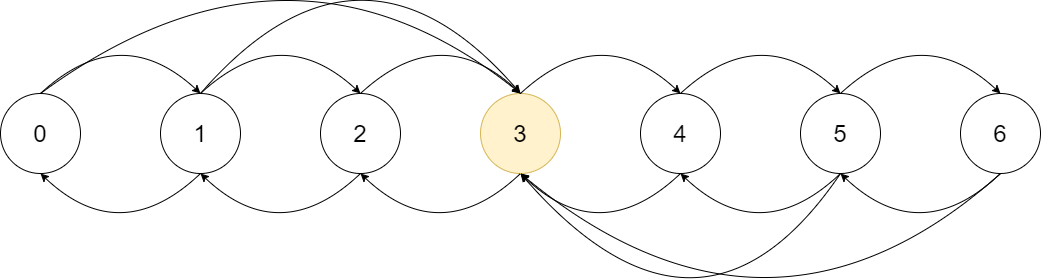
\includegraphics[width=\textwidth]{figures/navigationsystem-diagram/navigationsystem-cache-overview-2.png}
\end{figure}

\begin{figure}
\caption{Asynchronous navigation subsystem}
\label{fig:async.navigation}
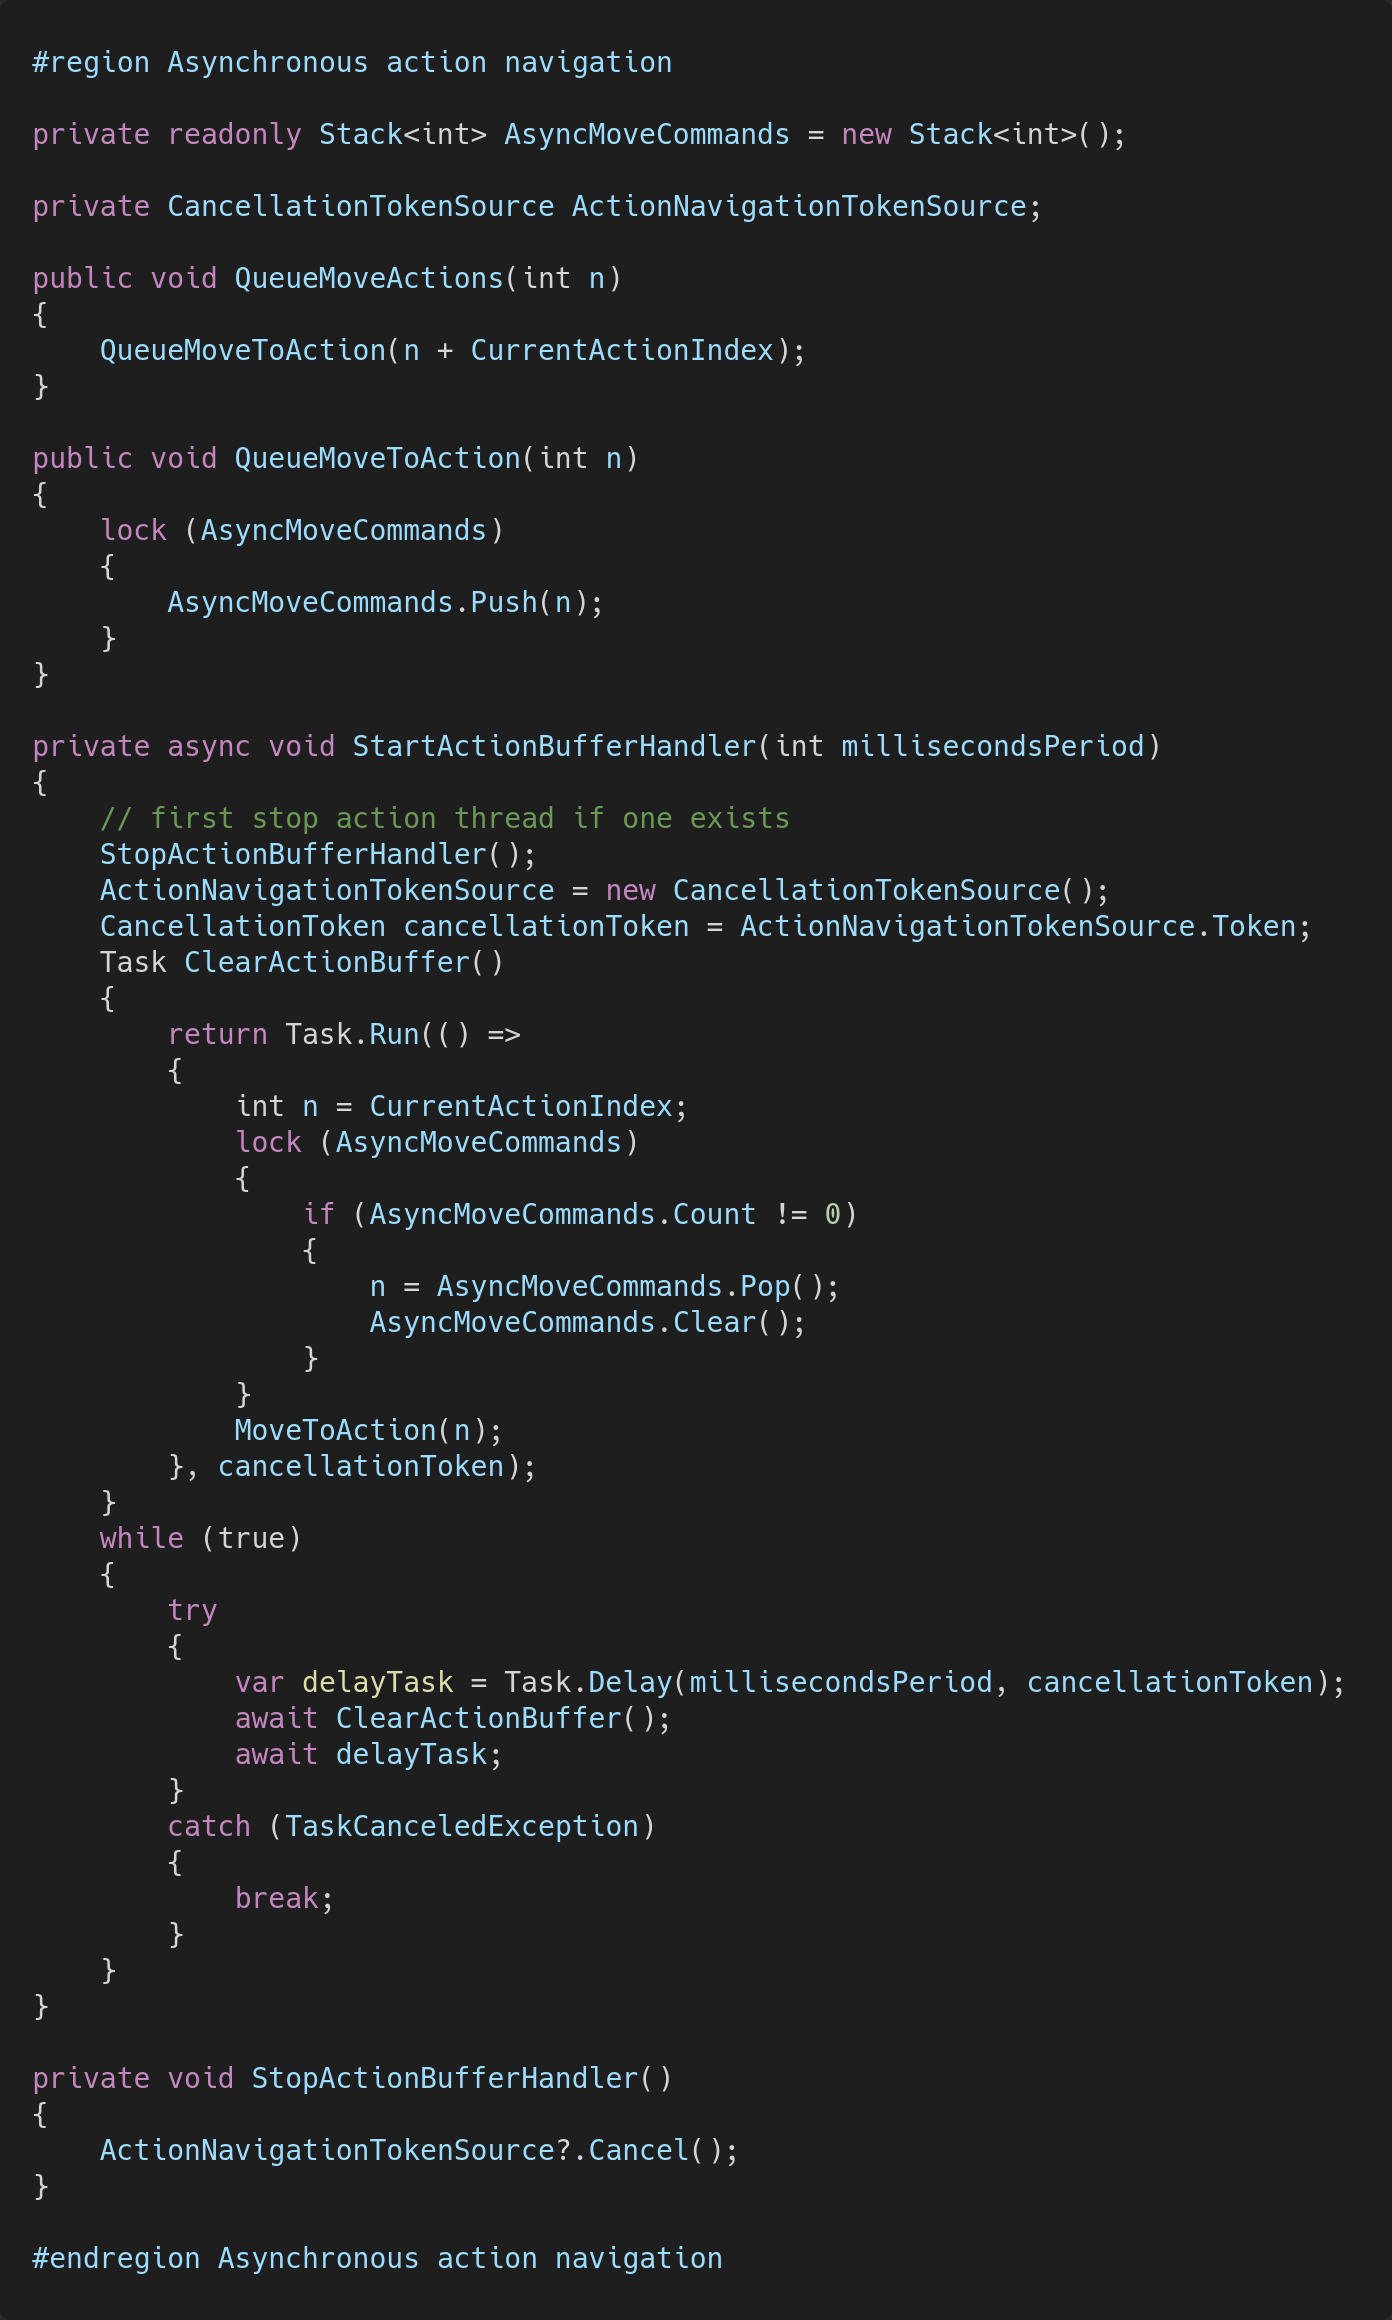
\includegraphics[width=\textwidth]{figures/code/nav-arch/async-navigation.png}
\end{figure}


\subsubsection{Centralized navigation system}

While implementing other features such as the diffusion, I noticed that having to implement for each page action the forward and backwards code, my code became quite error-prone. It was hard to notice bugs because it was not feasible to check every single action from both directions manually and creating a testing framework just because of this was out of scope. \\
Some navigation bugs were easy to find because due to the overall still linear nature of the navigation system, errors did propagate. This means that a error in a previous action most likely did break the page state on future actions because they depend on each other. \\
Nonetheless, this did not help in tracking down the bug because I did not know on which action the error happened. This only further incentivised me to reiterate on the navigation system again.


I summarized all the problems I currently had with my code which not only consisted of performance problems but also with visualization problems. Resizing the window did not appropriately scale the UI elements as can be seen in Figure \ref{fig:plugin.scaling.bug}. Additionally, the current navigation system was quite restricted in what kind of UI elements it supported without further hassle. Since I only updated the existing code during the last time I revisited the navigation system, the core design was still all about directly manipulating and creating UI elements on demand. The functions I wrote revolved around the UI elements I was using thus I could not reuse them if I wanted to use different UI elements; leading to the limited support of the navigation system I mentioned.

Essentially, the problem was that I used a lot of code-behind which was highly coupled to the XAML code. I did it like this because it was very straight-forward to do so and lead to fast results. At first, I thought the trade-off between loss of maintainability/flexibility in the future and not having to spend precious time to learn design patterns for WPF applications was worth it. I thought so because I was not writing an enterprise application on which the long-term success of a company depended and which would get regular updates in the future thus high maintainability or being easy to extend was not a priority. I got proven wrong when I realized I already reached the limit of "code smells" which slowed me down in updating, fixing or creating new features. What follows is the list of problems together with what requirement the new navigation system would need to meet to solve them:

\begin{figure}
\caption{Example for bad scaling property in previous plugin versions}
\label{fig:plugin.scaling.bug}
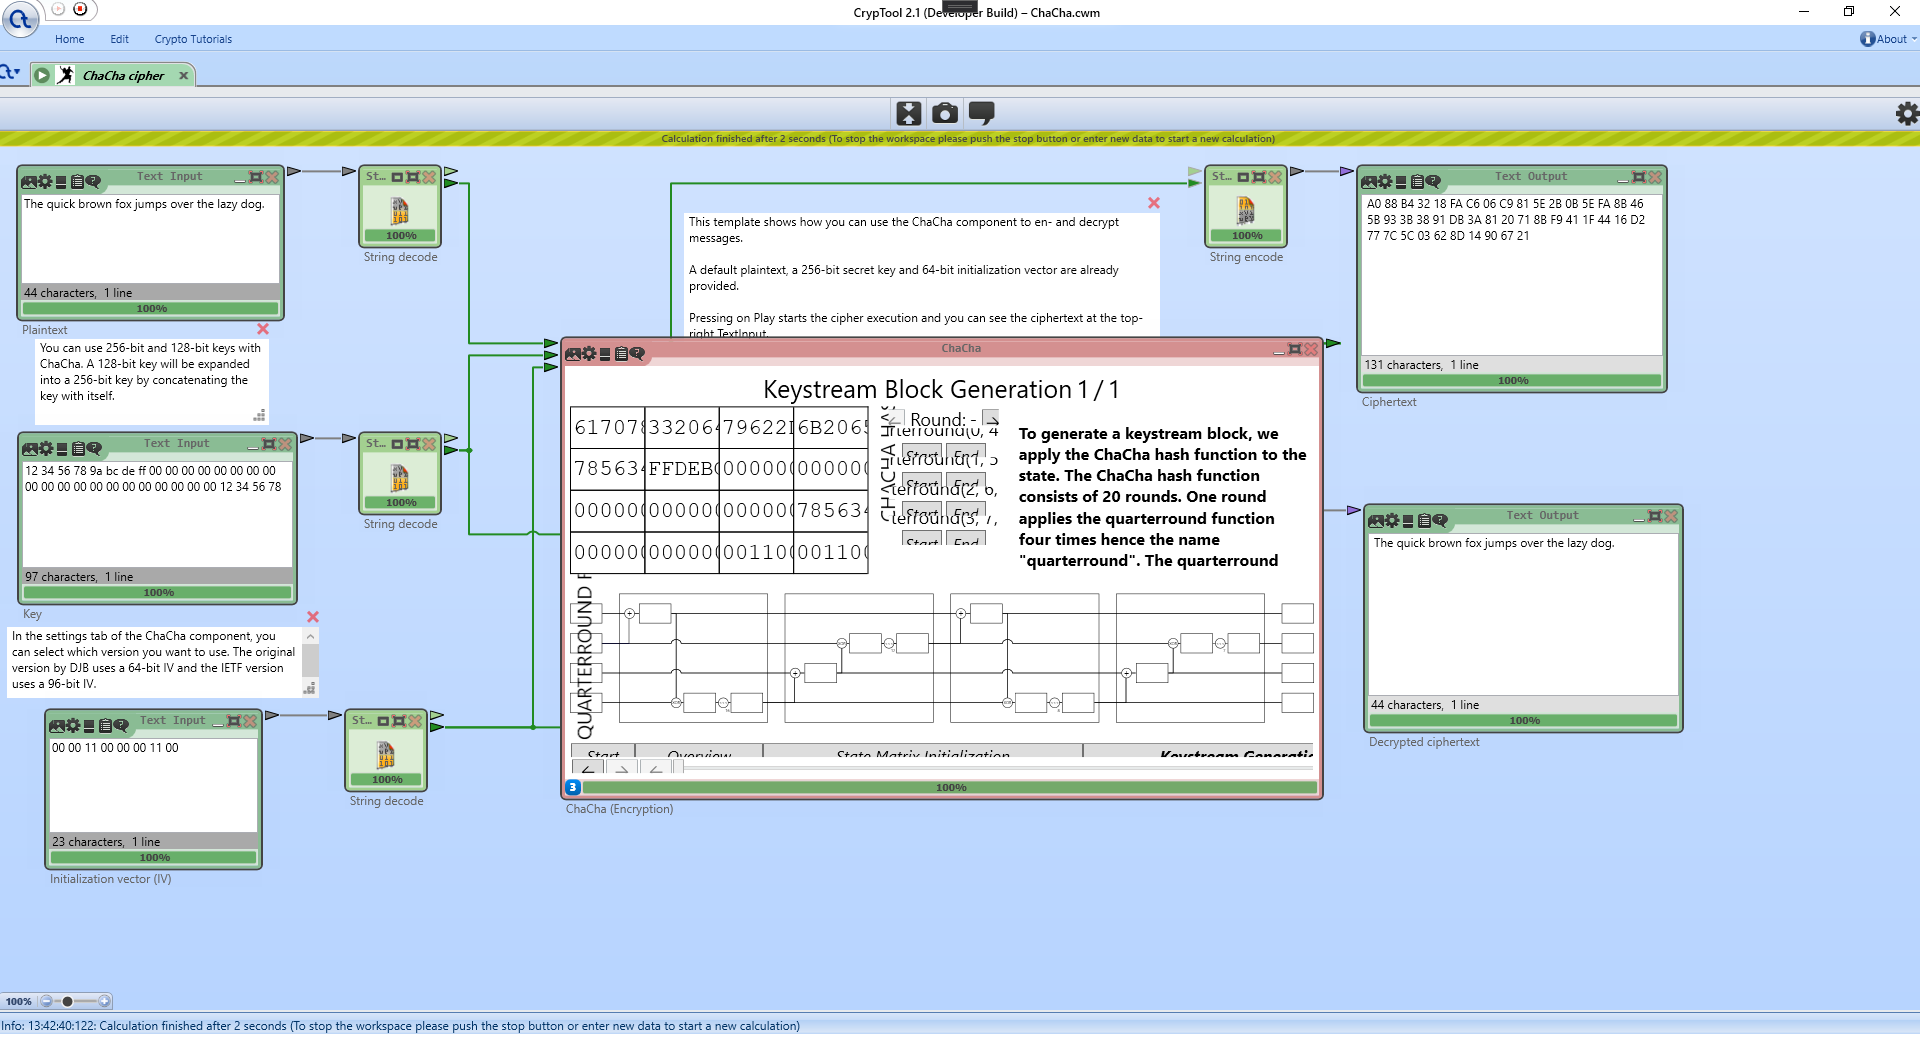
\includegraphics[width=\textwidth]{figures/ct2/scaling-bug-example.png}
\end{figure}

\begin{description}
\item [(Inconsistent) Performance] The underlying linear design was crippling the performance for the reasons already mentioned. The introduction of caches did only fight the symptoms but did not solve the main issue. Further, it made the performance confusing for the users since sometimes, it took close to no time at all to move to a certain action but on the other hand, it sometimes took quite a lot of time to move to a different action (because it was not cached). \\
\textit{\textbf{Requirement}}: Moving to any action should be done in $O(1)$. This means, it should not matter how many actions we needed to skip to arrive at the destination.
\item [Error-prone design for action creation] Writing new actions was error-prone because I needed to write code for forward and backwards navigation which introduced mental overhead because it depended on the code of all previous actions. This also lead to error propagation. Errors were easily noticeable by users but were hard to track down to their origin.\\
\textit{\textbf{Requirement}}: New actions should be able to be written without having to write backwards navigation code. Backwards navigation should be handled automatically and thus be "error-free by design".
\item [No coherent system design] Adding new code without following a design pattern made it hard to grasp the system architecture over the long run. Additionally, the high coupling of the backend (code-behind) with the frontend (XAML) made it harder to implement new features in one part without needing to modify the other part. The system essentially got very rigid and over time, even seemingly small changes took quite some time to implement.\\
\textit{\textbf{Requirement}}: The new system should make it clear what piece of code is responsible for what and thus be highly modular. This should also make it clear where new code must be added to implement a new feature without increasing technical debt; while also decreasing the possibility to introduce bugs since code is less coupled. To summarize, the new architecture should strive for high cohesion, but low coupling.
\end{description}
